%%==================================================
%% diss.tex for SJTU Master Thesis
%% based on CASthesis
%% modified by wei.jianwen@gmail.com
%% version: 0.3a
%% Encoding: UTF-8
%% last update: Dec 5th, 2010
%%==================================================

% 字号选项: c5size 五号(默认) cs4size 小四
% 双面打印(注意字号设置)
\documentclass[cs4size, a4paper, twoside]{sjtuthesis} 
% 单面打印(注意字号设置)
%\documentclass[cs4size, a4paper, oneside, openany]{sjtuthesis} 

% \usepackage[sectionbib]{chapterbib}%每章都用参考文献

\usepackage{algorithm}
\usepackage{graphicx}
\usepackage{array}
\usepackage{amsmath}
\usepackage{amssymb}
\usepackage{amsthm}
\usepackage{mathrsfs}
\usepackage{bm}
\usepackage{bbm}
\usepackage{bbold}
\usepackage{xfrac}
\usepackage{algorithmic}
\usepackage{upgreek}
\usepackage{multirow}
\usepackage{arydshln}
\usepackage{subfigure}

\newboolean{DOIT}
\setboolean{DOIT}{false}%编译某些只想自己看的内容,编译true,否则false

%% 行距缩放因子(x倍字号)
\renewcommand{\baselinestretch}{1.3}

% 设置图形文件的搜索路径
\graphicspath{{figure/}{figures/}{logo/}{logos/}{graph/}{graphs}}

%%========================================
%% 在sjtuthesis.cls中定义的有用命令
%%========================================
% \cndash 中文破折号
% 数学常量
% \me 对数常数e
% \mi 虚数单位i
% \mj 虚数单位j
% \dif 直立的微分算符d为直立体。
% 可伸长的数学箭头、等号
% \myRightarrow{}{}
% \myLeftarrow{}{}
% \myBioarrow{}{}
% \myLongEqual{}{}
% 参考文献
% \upcite{} 上标引用
%%========================================


\begin{document}

\renewcommand{\textfraction}{0.15} 
\renewcommand{\topfraction}{0.85} 
\renewcommand{\bottomfraction}{0.65} 
\renewcommand{\floatpagefraction}{0.60} 

%%%%%%%%%%%%%%%%%%%%%%%%%%%%%% 
%% 封面
%%%%%%%%%%%%%%%%%%%%%%%%%%%%%% 

% 中文封面内容(关注内容而不是形式)
\title{移动容迟网络中自适应路由算法的设计与实现}
\author{}
\advisor{}
\degree{硕士}
\defenddate{2015年6月16日}
\school{青岛大学}
\institute{信息工程学院}
\studentnumber{2012020406}
\major{}

% 英文封面内容(关注内容而不是表现形式)
\englishtitle{\XeTeX/\LaTeX\, Template for QDU Master Degree Thesis \version}
\englishauthor{\textsc{Lei You}}
\englishadvisor{Prof. \textsc{Changjiang Wei}}
\englishschool{Qingdao University}
\englishinstitute{\textsc{Information Engineering College} \\
  \textsc{Qingdao University} \\
  \textsc{Shandong, P.R.China}}
\englishdegree{Master}
\englishmajor{Software Engineering}
\englishdate{Jun. 16th, 2015}

% 封面
\maketitle

% 英文封面
%\makeenglishtitle



%%%%%%%%%%%%%%%%%%%%%%%%%%%%%% 
%% 前言
%%%%%%%%%%%%%%%%%%%%%%%%%%%%%% 
\frontmatter

% 摘要
%%==================================================
%% abstract.tex for SJTU Master Thesis
%% based on CASthesis
%% modified by wei.jianwen@gmail.com
%% version: 0.3a
%% Encoding: UTF-8
%% last update: Dec 5th, 2010
%%==================================================

\begin{abstract}

容迟网络的主要目标是支持具有链路间歇性连通、时延大、错误率高等通信特征的不同网络的互联和互操作。由于节点移动性、链路间歇连通、网络频繁割裂等特点,容迟网络中的源节点和目的节点之间在多数情景下不存在一条连通路径,因此节点采用“存储-携带-转发”的路由模式。
近年来,针对容迟网络的研究主要集中在路由协议领域,如何做出正确高效的路由选择是无线网络领域内的关键技术和主要研究课题。容迟网络路由协议根据消息副本在网络中的数量可以简单的划分为基于复制策略的路由协议和基于转发策略的路由协议。
%随着手机、平板电脑、PDA等手持设备的大量普及,引入社交网络分析技术,传统的容迟网络正在向社交容迟网络变迁,形成一类新兴容迟自组网。
本论文重点讨论如何设计用于移动容迟网络的高效实用的路由算法,
%由于容延网络中的节点具有高度移动性并且稀疏部署,这将导致容延网络中的拓扑结构动态变化以及链路时断时续,给路由设计带来很大的困难和挑战。此外,在不同的应用场景中,节点所能收集到的信息也各不相同,在这些场景中,需要节点利用收集到的信息,实现自适应的路由算法。
论文的研究工作主要集中于三点: 基于移动模式最优节点群组选取算法,基于消息传输收益的最优队列调度算法,以及基于跳数的启发式距离向量算法。其中基于移动模式的MPAR 算法从节点的移动记录中提取出节点 (群组) 的移动模 式,并利用节点共同常访地点预测消息的投递概率。MPAR 算法选取具有最优消 息投递概率的节点群组,证明了该问题的 NP-hard 难解性,同时指出了求解该问 题采用 online 算法的难度,并提出了启发式算法进行求解。在基于消息传输收益的队列调度算法的研究中,为了衡量每条消息的传输收益,定义了收益效用函数,并根据计 算出的每条消息的传输收益值,将该问题建模为组合最优化问题,并采用动态规 划(Dynamic Programming,DP)算法解决。对于基于跳数的启发式算法,利用网络中的数据包携带节 点之间平均跳数信息。定义了一个启发式函数用以估计消息距离目的节点所需的跳数。为了便于计算,将启发式函数的计算转化为矩阵乘法运算。

\begin{figure}[!b]
  \keywords{\large \textbf{机会网络\quad 容迟网络 \quad 路由协议 \quad 数据分发 \quad 优化算法}}
  \end{figure}
\end{abstract}



\begin{englishabstract}

The objective of the architecture for Delay Tolerant Network (DTNs) is to support the networking between nodes under the circumstance with intermittent connectivity, high end-to-end latency and high transmission error ratio. Due to the mobility of nodes, there usually does not exist an end-to-end connected path. Therefore, nodes in DTNs communicate in a hop by hop ``store-carry-forward'' manner. In recent years, research on DTNs mainly focused on routing protocols, and thus it becomes a hot topic in DTNs that how to make a correct and efficient routing strategy adaptively. The protocols in DTNs can be categorized into two types, replication based routing and forwarding based routing. The main contribution of this thesis are focused on three aspects, movement pattern-aware relay node group selection algorithm, message transmit profit based optimal schedule algorithm, and hop count based heuristic distance vector protocol. In the first aspect, we propose a Movement Pattern-Aware optimal Routing (MPAR) for SDTNs, by choosing the optimal relay node(s) set for each message. Concretely, the movement pattern of a group of node(s) can be extracted from the movement records of nodes. the routing problem is formally defined as a $NP-Complete$ combinatorial optimization problem.
We also demonstrate the difficulty for an online algorithm to solve the routing problem. 
In the second aspect, we try to improve the routing performance by resorting to an efficient data item selection mechanism that takes the bandwidth and connection duration time into consideration. A specific data item selection mechanism for a probability-based routing is devised, which is formally defined as an optimal decision-making problem and solved by the dynamic programming technique.
In the third aspect, we propose a hop count based heuristic routing protocol by utilizing the information carried by the peripatetic packets in the network. A heuristic function is defined to help in making the routing decision. We formally define a custom operation for square matrices so as to transform the heuristic value calculation into matrix manipulation. 

\begin{figure}[!b]
\englishkeywords{\large \textbf{opportunistic network; cellular network; routing protocol; data dissemination; optimization algorithm}}
\end{figure}
\end{englishabstract}


% 目录
\tableofcontents

\theoremstyle{plain}
\newtheorem{definition}{定义}
\newtheorem{theorem}{定理}
\newtheorem{lemma}{引理}
\newtheorem{proposition}{命题}
\newtheorem{postulation}{公设}

%%%%%%%%%%%%%%%%%%%%%%%%%%%%%% 
%% 正文
%%%%%%%%%%%%%%%%%%%%%%%%%%%%%% 
\mainmatter


%%引言
\begin{introduction}

容迟网络或者容断网络(Delay/Disruption Tolerant Networks, DTN)是近年来无线网络领域内的一个研究热点,泛指部署在极端环境下由于节点的移动或者能量调度等原因而导致节点间只能间歇性进行通信甚至长时间处于中断状态的一类网络\upcite{Spyropoulos:2010tc,王:2013wq,杨:2012vw}。其概念起源于星际网络 (Interplanetary Internet/IPN),主要目的是为了将因特网中的协议应用到星际之间的网络互联中\upcite{肖:2007um}。为此国际互联网研究任 务组(Internet Research Task Force, IRTF)专门成立了星际网络研究小组 (Interplanetary Internet Research Group/IPNRG)。 星际网络中消息传输的主 要问题是长传播时延,其过长的传播时延会导致现有的网络协议失效\upcite{Maitreyi2013,Miao2013,Martin-Campillo2013,Desta:2013gj,Wei:2013da,Shrestha:2013fj, Aijaz:2013gq}。非对称的 带宽以及低比特率等等也都给网络协议设计带来了非常大的困难和挑战\upcite{杨:2009tc,袁:2009vf}。

    在 2001 和 2002 年,IPN 的研究者初次尝试将 IPN 的架构应用于其它一些陆地 上的挑战性网络中,如用于发展中国家偏远地区通信和 Internet 接入服务的信息网 络、湖泊环境下的水声传感器网、野生动物追踪网络、以及高速行驶的车辆组成的 车辆 Ad Hoc 网络等\upcite{Spyropoulos2007,Brunner2005,Wang2007,Xu:2009fx}。这些网络具有间歇连接、时延极高、频繁割裂、非对称数据率、 安全性差、较高的误码率与丢包率以及异构互联等特性\upcite{Mahendran2013,Zhu2013a,Li2013,Talipov2013,Borrego2013,Gong:2013cy,Jiang:2013df}。然而与 IPN 不同的是,陆 地上的挑战性网络由于节点的强移动性等特点,其更加强调节点之间连接的频繁中断(Disruption),而 IPN 由于节点之间具有极远的距离,其更加强调节点之间传播的高时延(Delay)。在 2004 年,Kevin Fall 在 SIGCOMM 上提出了一种用于此类挑战性网络的一种架构方式,自此容迟网络引起了空前的广泛关注。随着相关研究成果不断涌现,Delay/Disruption Tolerant Network 这一名称逐渐被研究者们接受。此外,国际互联网研究任务组(Internet Research Task Force, IRTF)还专门成立了容迟网络研究小组(Delay-Tolerant Networking Research Group, DTRNG。研究者在DTN领域开展了广泛的研究工作与试验部署,其应用涵盖了传统Internet之外的许多通讯网络,例如英国的UK-DMC(United Kingdom Disaster Monitoring Constelation),瑞典的SNC(Sami Network Connectivity),以及在非洲实施的斑马监测网络,外太空的星际网络(Inter-planetary networks)、用于发展中国家偏远地区通信和Internet接入服务的信息网络、湖泊环境下的水声传感器网、以及高速行驶的车辆组成的车辆Ad Hoc网络等。目前,容延网络已经成为网络界最为热门的研究课题之一\upcite{Ferretti2013,Ginzboorg2013,Cha2013,Mtibaa2013a,Lin2013,Wei:2013dr,Wong:2013jx,Li:2013fl,Xiao:2013bv,Sundararaj}。

    为了实现这些异构挑战性网络间的互操作以及消息的可靠传输,DTN引入了捆绑层(bundle layer)\upcite{Ronan2011}并采用了保管传递(custody transfer)和存储-携带-转发(store-carry-forward)机制\upcite{Voyiatzis2012,Kumar2012,Parikh2005,Ott2005,Boloni:2011tj}。DTN作为未来互联网络发展的一个新方向,在环境监测、交通管理、水下探测和发展中国家偏远地区网络基础建设具有广泛的应用前景和实用价值。DTN主干网(DTNBone)是DTN的实现之一\upcite{Zhang2011},正如已经投入使用的多播主干网(MBone)一样,DTNBone的主要目的是建立一个世界范围的运行DTN协议的主机集合,又叫节点集,研究者可以依此开展有关DTN的各种研究\upcite{Flocchini2013,Baier:2012hb,Moreira:2012fa,Li2011,}。目前搭建DTNBone 使用的主要协议集主要有DTN2, ION, LTPlib, Spindle3, IBR-DTN等。为了从应用层的角度来研究DTN,研究者们在现有的DTN协议栈的基础上实现了几项有关应用,如Ohio University Simple Bundle Protocol API,DTN Tic Tac Toe Application,DTN新闻应用以及DTN摄像机。

如何做出正确高效的路由选择一直是无线网络领域内的关键技术和主要研究课题,然而传统的基于TCP/IP的Internet路由协议、移动Ad Hoc网络和无线传感网络的路由协议均很难在容迟网络中工作\upcite{Zhu2013,Conti:2014gg,Mehmeti:2014gt,Zhang:2014dj,Zhu:2014il,Wang:2014tt}。其原因是TCP/IP以及无线传感网络中的路由协议,其假设某一时刻存在一个稳定连通的端到端的通信链路, 但是这一假设在容迟网络中不再成立\upcite{Medjiah:2014hr,Xia:2013eb,Abdelkader:2013jl,WjHsu:2013vb,Jedari:2013uo}。由于容迟网络中的节点具有高度移动性并且稀疏部署,这将导致容迟网络中的拓扑结构动态变化以及链路时断时续,因此在某个时刻或者某段时间内不存在端到端的路径。正是由于传输链路的这种时变性和不确定性使得容迟网络中的路由研究是一项挑战性的课题,因此设计可靠有效的容迟网络路由算法来提高网络连接性、降低能量消耗和时延、增加消息投递率就成为容迟网络研究的一个核心问题\upcite{Rothfus:2013gj,Deng:2013fr,Wei:2013hc,Fan:2013fv}。容迟网络中的路由算法研究作为一项关键技术成为新一代无线通信网络研究领域备受关注的前沿热点课题\upcite{XinKang:2013ui,XiaoChen:2013to,Wu:2013tk,PUTournoux:2013th,Ciobanu:2013gb,Yuan:2013hj}。

    目前DTN的路由方面的研究主要可以分为单播路由及多播路由两类\upcite{Hu:2013tw,Zhu2013a,Anthonysamy:2013wf},迄今大部分的研究成果主要集中在单播路由上,多播路由近几年逐渐被研究者所重视。单播路由可以分为复制策略(naive replication strategy),转发策略(utility based forwarding strategy), 混合策略(hybrid strategy), 基础设施辅助策略(infrastructure assistance strategy)以及编码策略(coding based strategy)五种;多播路由主要可以分为基于域内(intra-domain)的多播路由和基于域间(inter-domain)的多播路由。然而通过对容迟网络路由算法相关的文献,特别是近几年来的主要研究成果进行了总结发现,目前部分路由算法中所采用的节点移动模型过于理想化,节点的移动模式单一,缺乏实用性;且在一些特殊环境中,能量及缓存是更大的限制,应当为此单独设计算法优化;部分路由协议缺乏多项评估指标的综合考虑,往往在个别指标上性能优越,但无法优化多项指标,网络整体性能难以获得极大的提升。 

    国内目前仍然处于跟踪研究的初始阶段,急需在这一领域展开必要的研究并取得实质性的成果。鉴于以上总结,目前亟需设计基于多策略的容迟网络路由算法研究,以克服目前容迟网络路由算法研究中所存在的局限性。 本课题拟从上文所述的局限性出发,结合具体的应用场景,设计并实现对网络环境变化自适应的路由算法。




\end{introduction}

%% 各章正文内容
\chapter{研究现状}

DTN为了实现这些异构挑战性网络间的互操作以及消息的可靠传输,引入了捆绑层(bundle layer)并采用了保管传递(custody transfer)和存储-携带-转发(store-carry-forward)机制。DTN作为未来互联网络发展的一个新方向,在环境监测、交通管理、水下探测和发展中国家偏远地区网络基础建设具有广泛的应用前景和实用价值。DTN主干网(DTNBone)是DTN的实现之一,正如已经投入使用的多播主干网(MBone)一样,DTNBone的主要目的是建立一个世界范围的运行DTN协议的主机集合,又叫节点集,研究者可以依此开展有关DTN的各种研究。目前搭建DTNBone 使用的主要协议集有DTN2, ION, LTPlib, Spindle3, IBR-DTN等。为了从应用层的角度来研究DTN,研究者们在现有的DTN协议栈的基础上实现了几项有关应用,如Ohio University Simple Bundle Protocol API,DTN Tic Tac Toe Application,DTN新闻应用以及 DTN摄像机。

DTN的路由方面的研究越来越受到国内外学者的重视,主要可以分为单播路由及多播路由两类,迄今大部分的研究成果主要集中在单播路由上,多播路由近几年逐渐被研究者所重视。单播路由可以分为复制策略(naive replication strategy),转发策略(utility based forwarding strategy), 混合策略(hybrid strategy), 基础设施辅助策略( infrastructure assistance strategy)以及编码策略(coding based strategy)五种;多播路由主要可以分为基于域内(intra-domain)的多播路由和基于域间(inter-domain)的多播路由。

\section{单播路由}
\subsection{复制策略}
复制策略的特点是节点在向中继节点进行消息复制时,不考虑中继节点的选择问题。常见的方法主要有洪泛(flooding)以及受控洪泛(controlled flooding)\upcite{Crowcroft2008}。著名的传染病(Epidemic)路由算法\upcite{Vahdat2000}是基于洪泛的一个代表性算法,该算法模仿生物环境中传染性病毒的传播方式,体现在DTN中,每个节点维护一个消息总结向量,当两个节点能够连接时通过交换消息向量来彼此交换缺少的消息。然而过度冗余的消息副本会带来网络拥塞,从而增大时延和丢包率。文献\upcite{Grossglauser2002}提出的Direct Delivery(DD)算法则可被视为是基于洪泛的另一个极端情况,该算法同样不考虑中继节点的选择——不向任何中继节点复制消息,每个节点只将消息直接传递给目的节点,故具有很低的投递率,只作为研究路由算法的一种参考。文献\upcite{Grossglauser2002}还提出了一种两跳中继多次复制(Two-Hop-Relay)的路由策略,源节点将消息复制给与其关联的T个邻居节点,这些邻居节点不再进行复制操作,而是将这些消息直接传输至与之有关联的目的节点。文献\upcite{Spyropoulos2005}提出了Spray and Wait算法,源节点持有T份拷贝,并向遇到的节点分发所持有的拷贝,若节点持有的拷贝数量大于1,则继续进行分发,当节点只持有消息的一个拷贝时,采用DD算法将消息传输到目的节点。文献\upcite{Spyropoulos2007a}给出了一种特殊的“Spray”方法,每次分发一半的拷贝给第一个遇到的节点,使整个Spray阶段呈二叉树状,当节点移动独立同分布时,其期望时延最优。

\subsection{转发策略}

单纯使用转发策略的路由,往往也称为单副本路由,是根据网络的拓扑知识来指定一个或几个用于衡量节点作为中继转发某消息的合适程度或链路的传输时延等的效用指标,制定效用指标的目的,往往是为了在选路过程中优化某一个或者某几个目标。单副本转发策略必须确保据此所选出的中继节点能够比源节点更好的胜任消息投递工作,如果可以设定出能够准确描述节点属性的效用指标,则可以保证在网络中只有一个消息的副本在传输时达到一个较为理想的投递率,保证可靠传输。目前除了星际网络之外,很少有能够预测节点移动以及网络拓扑变化,这给指定精确效用指标带来了困难。文献\upcite{Jain2004}提出的适用于星际网络的路由算法是该策略的典型代表,它将容迟网络建模为有向多重图,将网络的动态拓扑信息抽象为知识ORACLE集。以知识ORACLE作为路由问题的输入,研究路由算法性能与ORACLE间的关系。ORACLE分为接触总结、接触、排队和流量需求四种类型,根据所需ORACLE的不同,文献\upcite{Jain2004}提出了FC、MED、ED、EDLQ、EDAQ和LP共六个算法。其中FC算法最简单,基于零知识输入,以时间作为效用指标,每个节点选择与自己接触最早的节点进行转发。其它五个算法的效用指标都是基于链路状态时延而指定的,根据能够利用的ORACLE知识的多少,效用指标的准确程度也不同,MED算法基于网络中的节点接触总结,采用Dijkstra算法求解最优路由,由于节点接触总结信息是固定的,故该算法不是一个自适应路由算法,从这种意义上讲,若网络情况稍有变化,则效用指标就不再能准确反映网络情况。ED算法则根据网络中所有节点的接触信息采用改进的Dijkstra算法求解最优路由。而EDLQ和EDAQ路由算法则是在ED算法的基础上分别引入局部节点缓存队列和全局缓存队列信息,进一步优化性能。而LP路由算法则进一步的引入了流量需求,将最优路径转化为一个线性规划问题进行求解,然而这种方法可行性不足,主要作为研究参考。文献\upcite{Guo2013}提出的PASR(Prediction Assisted Single-copy Routing)收集并维护在较短时间内获取的网络连接信息,然后使用一个离线的贪心算法求解出底层网络移动性的有关特点,描述出最优路径所具有的特点并依此给出一个有效利用历史信息的导引方法,PASR根据此方法,利用一个在线算法来计算路由。为了取得较好的网络性能通常需要全局或者部分总结的拓扑信息,而这些信息在大部分强调节点随机移动性容迟网络中往往不可能预先获知,这就要求网络中节点按需(on-demand)获取网络拓扑,,目前常用的方法是依靠一个链路状态协议(link state protocol)进行拓扑知识分发。文献\upcite{Jones2007}提出的MEED算法即是如此,其进行路由所需要的全局链路拓扑信息单独由一个链路状态协议维持。MEED在MED算法之上做了改进,MED算法假设网络中的拓扑知识集能够获得,然而在实际的情况中可行性不大。MEED基于滑动窗口对链路的期望时延进行评估,文献\upcite{Jones2007}还提出了一种与源路由和按需路由不同的一种路由策略,即逐跳路由(per-hop routing),利用该策略能够更好的利用最近所出现的可用链路。

\subsection{混合策略}

与基于复制策略的路由算法以及只利用单拷贝转发策略的路由算法相比,混合策略的路由算法更为灵活,既利用了复制策略多副本的并行性,又优化选择了较为合适的中继节点。文献\upcite{Spyropoulos2007a}提出的Spray \& Focus算法是一种典型的混合策略路由算法,在Focus阶段,算法实行聚焦搜索,有选择的进行副本的转发投递。文献\upcite{Erramilli2008}提出的授权转发(delegation forwarding/DF),将DTN中路由问题转化为停止问题(stopping problem)进行研究,其基本策略是对节点定义效用函数,用以描述节点对于转发某消息的合适程度,每当进行一次复制操作后,两个节点都将更新自己的效用函数,从而使今后选择转发节点的指标越来越严格,有效的控制了副本的数量。该文献证明了,采用授权转发协议产生的副本数量可由$O(n)$降低到$O(\sqrt{n})$。文献\upcite{Liu:2009uy}提出的OOF(Optimal Opportunistic Forwarding)算法结合了跳数和副本存活时间来定义了副本的投递概率,并利用最优停止理论递推的对投递概率进行计算,获得期望上的最优投递率。由于OOF算法中,其需要维护的投递概率表是四维的,计算及更新起来具有较大的开销,为了解决此问题,文献\upcite{Liu:2009uy}还提出了OOF—算法,即不再考虑副本存活时间,从而使概率表降低一维,模拟实验表明其表现只略微弱于OOF算法。文献\upcite{Burns:2005gi}提出的MV(Meetings and Visits)则利用节点间的相遇概率来描述消息传输的成功概率,任意两个节点间的相遇概率作为这对节点的传输概率,在此基础上通过递归的方式计算多跳传输的成功概率。两个节点相遇时,交换各自的消息以及传输概率信息,通过比较,节点仅向传输概率更高的中继节点复制消息。文献\upcite{El-Azouzi2013}将进化策略(Evolutionary Games)用于非合作性的受控转发(controlled-forwarding)中,在这种方法中,节点可以选择不同的策略来作为中继节点参与转发,引入效用函数来权衡期望收益和能量消耗,文献\upcite{El-Azouzi2013}证明了该方法可以以一种非集中式的方式进行,故适用于容迟网络选路。


\subsection{基础设施辅助策略}
基础设施辅助策略路由算法采用特殊的移动节点来负责容迟网络中节点间的消息寻路和传输,这些特殊节点通常称之为消息渡船(message ferry)和数据骡子(data mule)。这些节点通过控制自己的移动行为,按照一定的移动路线在网络相互割裂的区域进行移动,以“存储-携带-转发”(store-carry-forward)的方式辅助进行网络的消息转发,提高消息投递率。文献\upcite{Zhao2004}提出的MF(Message Ferry)算法是基于拓扑知识策略的典型代表,该算法通过引入一个称为消息渡船的特殊移动节点并通过规划该节点的移动路线,协助区域间的消息传输。作为MF的扩展,文献\upcite{Zhao2005}提出了四种方法,考虑了引入多个消息渡船的网络,以满足流量需求且传输延迟最小为优化目标,计算出消息渡船的最优移动路线,这四种方法分别为单路由算法(SIngle Route Algorithm/SIRA),多路由算法(MUlti Route Algorithm/MURA),节点中继算法(Node Relaying Algorithm/NRA)以及渡船中继算法(Ferry Relaying Algorithm/FRA)。文献\upcite{Zhao2005}还从另一个角度审视了其所提出的MF算法, 所改进的方法是不引入任何受控辅助接点来引渡消息,其所需要的渡船节点是由网络中原有节点选举产生的。文献\upcite{Zhang:2007bq}基于旅行商问题(Travel Salesman Problem/TSP)提出了另外一种渡船算法,其核心主要侧重于设计引渡节点路由,从而平衡消息传递率以及节点有限的缓存资源。文献\upcite{Banerjee:2007hm}所利用的投掷盒(Throwbox)是一种低成本,电池驱动的短程小存储量设备,由于其易于部署,故很适合用作引渡节点。当两个不同的节点都经过投掷盒所覆盖的范围时,先到达的节点可以把消息缓存在其中,以便将该消息传输到后到达的节点,这实际上也是一种保管传输策略。辅助节点的部署问题也是一个难点,文献\upcite{He:2010ks}提出的一种方法,其将传输时延和副本数目纳入考虑之中,结合效用函数利用贪心法选择位置来进行辅助节点部署,该算法具有二次多项式的时间复杂度。


\subsection{编码策略}
编码策略实质上是对DTN间歇连接特性予以补偿的一种机制,其并非是一种路由策略,但可以和其它常用路由策略混合以提高投递率。常见的编码策略有网络编码和擦除码,前者允许中继节点对消息进行编码,而后者只允许源节点对消息进行编码。文献\upcite{Wang:2005ka}使用了擦除码和复制策略来进行路由,在简单的复制策略中,消息会从源节点传给r个中继节点,而使用纠删码后,会产生kr个同等大小的编码块,并将复制给kr个中继节点,与普通的复制路由策略相比,加入了擦出码策略的方法采用了更多的中继节点,只要这些中继节点中有多于k个节点具有更小的延迟,则其表现就超过只用普通的复制策略的路由,其本质即是在消息所需总带宽不变的情况下增加其之间的并行性。文献\upcite{Jain2005}使用网络编码结合概率算法进行路由,当消息到达中继节点时,会被中继节点与其它接受到的消息混合进行线性编码产生一个新的消息,目标节点收到消息时再进行解码,从而减少消息传输的次数,提高消息分发概率。


\section{多播路由}
多播路由可以分为基于域内(intra-domain)的多播路由和基于域间(inter-domain)的多播路由。文献\upcite{Zhao2005a}是域内多播协议的典型代表,首先定义了三种多播语义模型,进而提出了五种路由算法:分别是基于静态树多播路由(static tree-based routing,简称STBR),基于动态树的多播路由(dynamic tree-based routing,简称DTBR),基于转发组的路由(GBR)、基于广播的多播路由(BBR)和基于单播的多播路由(UBR),并研究这些路由算法随着组成员知识ORACLE的不同而产生的性能变化。DTBR算法通常需要全局的拓扑知识来构建一个动态多播树,并且树中每个中间节点的多播成员接收列表由其上游节点决定,这一特点决定了DTBR算法不能很好地利用现有新出现的消息投递机会。为了克服这一缺点,文献\upcite{Ye2006}提出了OS-Multicast算法,该算法是一种基于动态树的按需式情形感知多播路由算法,动态树的每个中间节点维护一个所有多播成员的接受列表,以更好的利用最新出现的投递机会,但代价是网络中会有多余的多播消息副本在传输。文献\upcite{Chuah2009}提出了CAMR(Context Aware Multicast Routing)算法,该算法是一种基于节点密度的自适应多播路由算法。该算法试图通过获得一些额外的网络知识例如节点的速度和位置以获取更好的网络性能,同时该算法综合利用了节点的高发射功率和消息渡船机制以取得更高的消息投递率。文献\upcite{Wang:2012up}提出了一种基于动态多播树非复制策略的多播路由算法,该算法提出了比较-分割原则(compare and split)并同时利用节点的活动率水平(active rate level)和接触率水平(contact rate level)来指导动态多播树的构建。文献\upcite{Gao:2009wf}第一次提出基于社会网络(social network)的相关技术来研究容迟网络中的多播问题,该文献利用社会网络中的两个关键概念:社区(Communities)和聚集性(Centrality)计算DTN多播过程中的中继节点选择问题,并最终将该问题统一为常见的背包问题(knapsack problem)。基于域间的多播路由算法通常在每个DTN区域选择一个称为域首(domain leader)的节点来负责此区域多播消息的汇总和分发,这样整个DTN区域可划分为两层:域首层和域层。多播过程分为三步:(1)源节点将消息通过域内多播协议发送至源区域所在的域首,(2)源域首经过域间多播协议将消息传送至多播接收成员所在的各个区域的域首 (3)各个接收节点域首再经过域内多播协议传送至多播目的节点。文献\upcite{Ye:2007cf}所提出的SHIM(scalable hierarchical inter-domain multicast)算法和文献\upcite{Yang:2008hn}所提出的FBIMR(ferry-based inter-domain multicast routing)算法是典型的域间多播路由算法。
除了上述所提的路由算法外,还有不少与路由直接或间接相关的研究成果,例如芬兰赫尔辛基理工大学开发的the ONE(Opportunistic NEtwork Simulator)模拟器\upcite{Keranen2009},该模拟器用于对DTN中的路由算法性能进行仿真、模拟和验证。文献\upcite{Talipov2013}以智能手机系统为基础,利用存储-携带-转发方法,设计了基于bundle协议的信息分享的方法,该方法有效的降低了CPU以及电池的负载。

通过对容迟网络路由算法相关的文献,特别是近几年来的主要研究成果进行了总结发现:(1)复制策略可以增大消息的并行性和传递可靠性,有效的受控洪泛能够大大改善挑战性网络中的路由表现。(2)目前部分路由算法中所采用的节点移动模型过于理想化,节点的移动模式单一,缺乏实用性。(3)目前路由协议主要致力于优化投递率及传输实验,然而在一些特殊环境中,能量及缓存是更大的限制,应当为此单独设计算法优化(4)目前的路由协议缺乏多项评估指标的综合考虑,往往在个别指标上性能优越,但无法优化多项指标,网络整体性能难以获得极大的提升。因此需要利用新的分析工具研究容迟网络路由,同时考虑多个设计目标进行优化,建立基于多目标优化的高效路由协议.例如,以节点能量消耗、时延、传输率为目标,进行多目标决策,设计出最优路由协议。(5)国内目前仍然处于跟踪研究的初始阶段,急需在这一领域展开必要的研究并取得实质性的成果。鉴于以上总结,目前亟需设计基于多策略的容迟网络路由算法研究,以克服目前容迟网络路由算法研究中所存在的局限性。 

\chapter{论文工作总览}

论文主要研究工作集中于\ref{chap:基于移动模式最优节点群组选取的路由算法}、\ref{chap:基于消息传输收益的最优队列调度算法}、\ref{chap:基于跳数的启发式距离向量算法}三章。

\begin{itemize}
\item 第\ref{chap:基于移动模式最优节点群组选取的路由算法}章\footnote{该章研究内容已于2014年9月录用于SCI源刊\textit{Ad Hoc Networks},将于2015年1月发表}提出了一个用于社交容迟网络的机会路由算法(Movement Pattern-aware Routing, MPAR)。MPAR算法从节点的移动记录中提取出节点(群组)的移动模式,并利用节点共同常访地点预测消息的投递概率。MPAR算法选取具有最优消息投递概率的节点群组,证明了该问题的NP-hard难解性,同时指出了求解该问题采用online算法的难度,并提出了启发式算法进行求解。主要技术方案如下:
\begin{enumerate}
\item \textbf{维护节点移动记录矩阵,提取节点移动模式,求预测投递率}。利用节点手机的移动记录信息,从中提取节点(群组)移动模式,并以此为依据选出最优中继节点群组。利用移动模式对应的共同常访地点集合,可求出消息的预测投递率。

\item \textbf{证明最优节点群组的求解为$\mathcal{NP}$难类问题}。
将子集和问题归约为节点群组选取问题的一个特例,从而证明了该问题的$\mathcal{NP}$难解性。

\item \textbf{基于tabu-search, 提出了启发式算法求解最优节点群组}。该章提出了两种路由算法:基于局部搜索的Local-MPAR以及基于禁忌搜索的Tabu-MPAR。其中Tabu-MPAR较Local-MPAR能够较为有效的跳出局部最优陷阱。
\end{enumerate}


\item 第\ref{chap:基于消息传输收益的最优队列调度算法}章\footnote{该章研究内容已于2014年4月发表于SCI源刊\textit{International Journal of Distributed Sensor Networks}}设计了一种考虑带宽和链接持续时间的数据选择机制入手,尝试提高路由算法的性能。为了衡量每条消息的传输收益,定义了收益效用函数,并根据计算出的每条消息的传输收益值,将该问题建模为组合最优化问题,并采用动态规划(Dynamic Programming,DP)算法解决。主要技术方案如下:
\begin{enumerate}
\item \textbf{从消息投递率入手,为消息的每次传递定义收益值}。对于任意一对节点$a$和$b$, 分别计算出两节点共同持有消息副本时的投递概率,以及只有单一节点持有该消息时的投递概率,求差值以计算出本次传输的收益,为数据项在缓存中的调度提供参考依据。
\item \textbf{综合考虑带宽和节点间的接触持续时间,将数据选择问题建模为组合最优化问题}。结合第一点中所计算出的传输收益,以及节点的传输带宽和节点间的接触持续时间,把数据选择问题建模为组合最优化问题,并采用动态规划(Dynamic Programming,DP)算法解决.
\end{enumerate}

\item 第\ref{chap:基于跳数的启发式距离向量算法}章\footnote{该章研究内容已于2014年6月发表于SCI源刊\textit{The Scientific World Journal}}提出了一种基于跳数的启发式路由算法,并利用网络中的数据包携带节点之间平均跳数信息。定义了一个启发式函数用以估计消息距离目的节点所需的跳数。为了便于计算,将启发式函数的计算转化为矩阵乘法运算。
主要技术方案如下:
\begin{enumerate}
\item \textbf{尝试利用数据包来携带节点之间的跳数信息}。具体而言,在数据包头部写入该数据包所经过的节点,并记录节点与节点之间跳数。由此,当任意一条消息到达某节点时,利用\textbf{滑动窗口(slide-window)}技术更新其所记录的距离其它节点的平均跳数信息。

\item \textbf{定义启发函数用以估计消息从某节点到达其目的节点所需要的跳数}。函数如$
\label{eq:Hh}
\mathcal{H}(i,k) = hop(k) + h(i, d)
$其中$\mathcal{H}(i,k)$代表消息$k$若经过节点$i$到达目的节点$d$所需要的总跳数,由两部分组成:$hop(k)$代表消息$k$在到达节点$i$之前所经过的跳数(实际跳数),$h(i,d)$表示从当前节点$i$到目的节点$d$估计所需要经过的跳数(估计值)。

\item \textbf{将启发函数部分(即第二点中的$h(i,d)$部分)的计算转化为矩阵乘法问题。}将网络中节点建模为图论中的点,节点间的平均跳数信息建模为图论中的边权值,且为无向带权图,则该带权图表示为矩阵之后,可以利用矩阵相乘的方法求出$h(i,d)$的值,使运算更加简便。
\end{enumerate}
\end{itemize}
\chapter{基于移动模式最优节点群组选取的路由算法}
在许多节点具有一定社会属性的机会网络中,具有共同兴趣的移动用户往往访问一些与其兴趣相关的地点。研究表明,50\%的移动用户会在某一个特定的接入点(access point, AP)上花费约74\%的时间\cite{Henderson:2004ul}。换言之,节点往往具有频繁访问某一或某一部分地点(简称为常访地点)的特点。这些常访地点可被看做``连接''这些节点的枢纽。可以通过在常访地点部署缓存设备,用以辅助消息传递,例如投掷盒(throw-box)\cite{Ibrahim:2009we}等设备。缓存设备具有普通移动节点不具备的优势。首先,由于部署的缓存设备位置固定在常访地点,且节点往往在常访地点停留一段时间,所以节点与缓存设备之间具有比移动节点之间更加稳定的连接。其次,这些固定的缓存设备,没有如同移动节点那样便携性的限制和要求,故其存储容量往往比移动节点要大许多。由此,可以利用在常访地点部署缓存设备作为中继枢纽,从而提升机会网络中路由算法的性能表现。

本章研究多副本单播机会路由算法,基本假设如下。每条消息具有一对“源—目的”节点对(source-destination node pair),并且每条消息可在网络中具有多份拷贝。不同于以往基于社会网络分析求解社会关系的方法,或自定义社会属性的方法,本章利用节点收集的移动记录信息,从中提取出节点(群组)移动模式,并以此为依据选出最优中继节点群组。基本思想为:将持有某一条特定消息(或其拷贝)的任意一组节点看成一个整体,从记录信息中提取出移动模式,从而确定该节点群组的常访地点集合$A_1$。目的节点的常访地点$A_2$,也以相同方法获取。进而,取交集求得$A=A_1\cap A_2$,作为该节点群组与目的节点的共同常访地点集合。利用集合$A$,可以求出消息的预测投递率。路由目标即为求得能使预测投递概率最大的节点群组。此外,超出有效期(deadline)的消息不再具有价值,在求解移动模式的过程中,消息的时效性也被考虑在内。本章基于节点的移动模式,提出构造最优节点群组作为中继节点群的移动模式相关最优路由算法(Movement Pattern-Aware optimal Routing, MPAR)。就目前掌握的资料来看,这是首次利用节点群组移动模式进行社会相关的路由算法研究。

本章组织如下:第\ref{chap3:系统模型及基本定义}节引入系统模型及基本定义;第\ref{chap3:路由问题概览}节分析路由问题背后蕴含的两个关键属性,并给出最优路由问题的形式化定义;第\ref{chap3:搜索问题分析}节证明了该最优问题的计算复杂性,并提出了启发式算法用以求解近似最优解;第\ref{chap3:最优化路由算法}节给出路由算法的详细过程及描述;第\ref{chap3:仿真实验}节对仿真实验结果进行分析;第\ref{chap3:本章总结}节总结本章内容。

\section{系统模型及基本定义}
\label{chap3:系统模型及基本定义}

\begin{figure}
\centering
\subfigure[节点a向投掷盒发送消息\label{paper-MPAR/send_to_box}]
{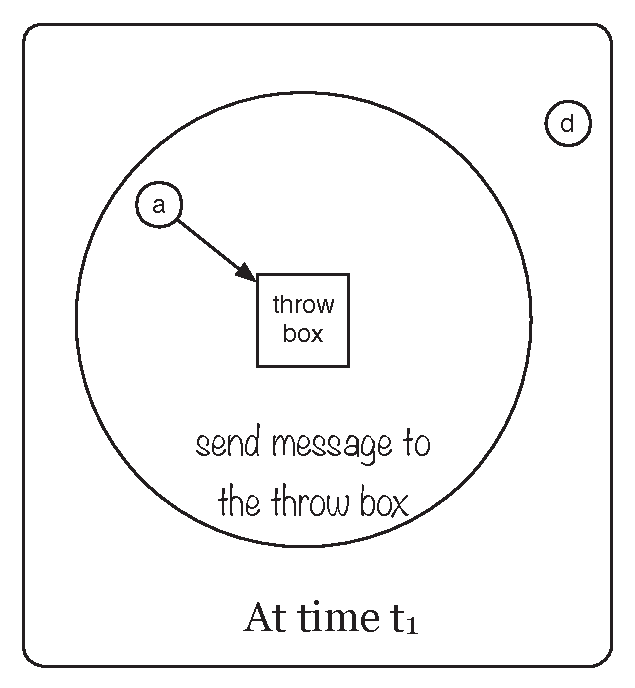
\includegraphics[width=0.4\linewidth]{paper-MPAR/send_to_box}}~~~~~~
\subfigure[节点d从投掷盒接受消息\label{paper-MPAR/receive_from_box}]
{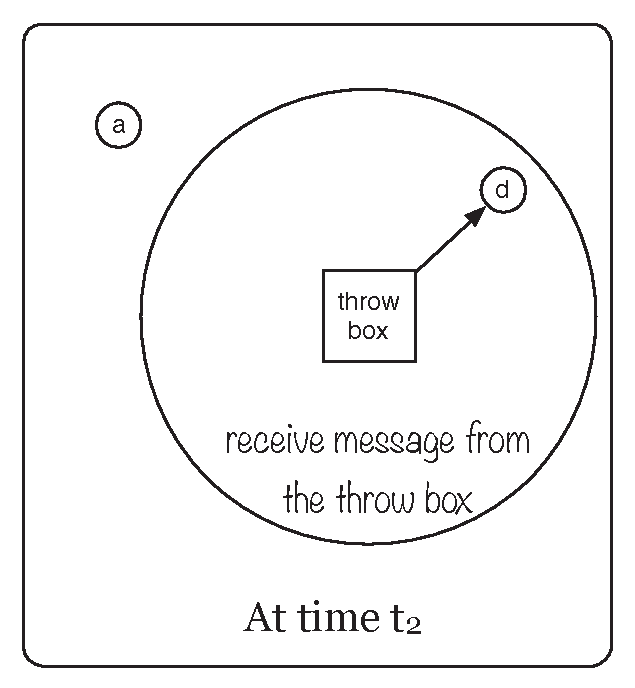
\includegraphics[width=0.4\linewidth]{paper-MPAR/receive_from_box}}
\caption{利用投掷盒完成消息从节点a到节点d的传递操作.}
\label{fig:chap3_box}
\end{figure}

\subsection{网络模型}

网络节点集合记为$\overline{N}\triangleq\{n_i|1\leq i\leq n\}$. 节点在给定的地点集合间移动,地点集合记为$\overline{A}\triangleq\{a_j|1\leq j \leq m\}$. 任意一个节点$n_i$的常访地点集合$A(n_i)\subseteq \overline{A}$. 该模型源于真实的移动网络,一个典型的实例是Dartmouth College的Wi-Fi Campus Network \cite{Jedari:2013uo}。另一符合该模型的一类网络是VANET。在VANET中,大量的公交车,电车等在车站等固定地点间移动。我们假设节点$n_i$访问任意一个地点$a_j$的时间间隔服从指数分布。此外,在任意地点内都部署有一个投掷盒装置,用于接受,缓存及传递消息。在此模型中,投掷盒的缓存容量假设为足够大,即在投掷盒中不会因缓存满而产生消息丢弃。如\figurename~\ref{fig:chap3_box}所示,节点a在$t_1$时刻将消息托管给投掷盒,在$t_2$时刻,该消息的目的节点d进入投掷盒的传输范围内,并从投掷盒接受该消息,至此,消息的投递操作完成。

我们假设每条消息$l$都具有一个值$\tau_l$,代表消息$l$在网络的剩余生存时间。随着时间消逝,$\tau_l$的值逐渐减少,当$\tau_l=0$时,该消息将从节点缓存中删除,不再存在于网络中。消息的生存时间属性,一定程度上避免了消息在网络中停留的时间过长。此外,应用程序所产生的消息因具有时效性,往往也会对消息设定一个生存时间。例如新闻发布或者广告发布服务,消息只在一定时间内有效。当消息超出某个时间即不再具有投递价值。




\subsection{基本定义}

由于作为手持设备的节点附属于具有社交属性的人群,节点的移动模式具有一定的周期性。举例而言,Smith先生在周一到周五上班,故其常访地点可能包含家,办公室,某些公交站点及一些快餐店等。周末,Smith先生通常去健身俱乐部或咖啡馆,或者一些不同于工作时间去的地方。然而,他的行为通常以一星期为一个周期,在一定程度上重复,即其移动记录具有一定的周期性。假设周期为$T$,若将$T$划分为$h$个时间槽,则每个时间槽的长度为$\frac{T}{h}$。将这些划分好的时间槽的边界时间点,用序列$<t_0,t_1,t_2,\ldots,t_h>$表示,则任意两个区间点$t_s$与$t_e$($t_s<t_e$)形成时间区间$[t_s,t_e]$,如图\figurename~\ref{fig:chap3_time_slots}所示。针对时间区间$[t_s,t_e]$,可以从节点的移动记录中,提取出对应的移动模式。节点的移动记录见定义\ref{def:移动记录}。

\begin{figure}[!t]
\centering
  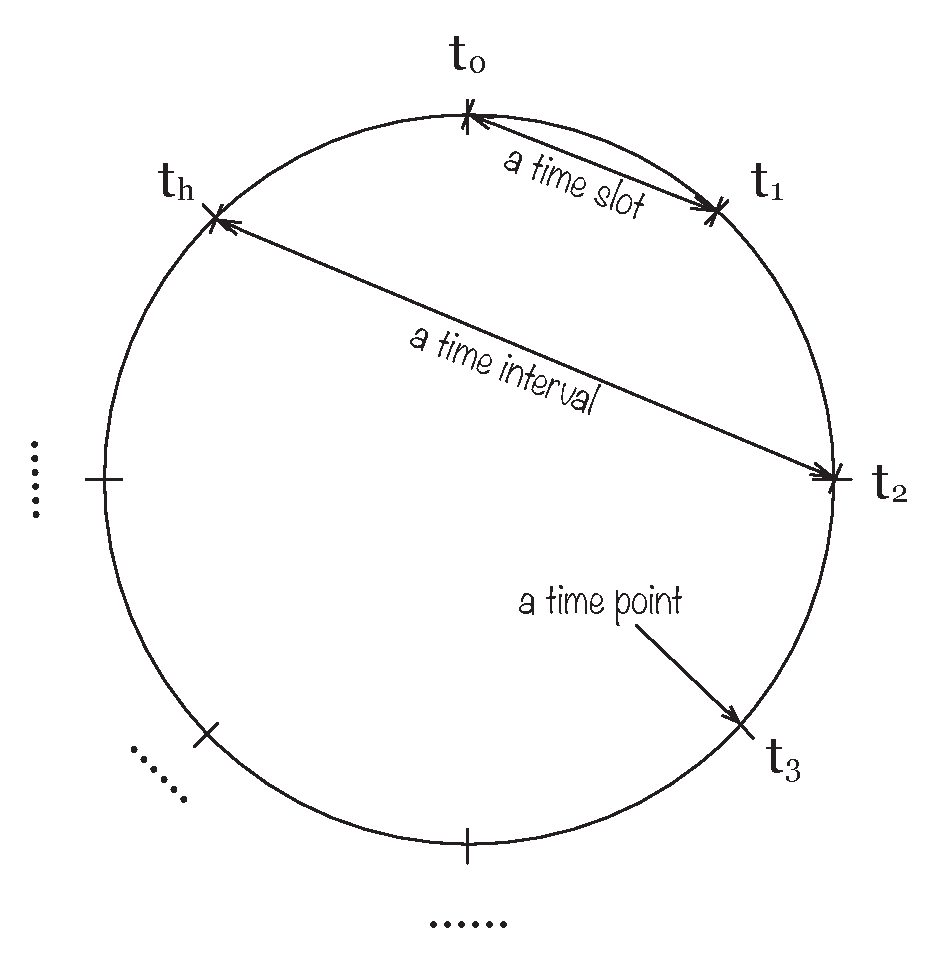
\includegraphics[width=0.55\linewidth]{paper-MPAR/time_slots}
  \caption{周期$T$划分为$h$个时间槽}
  \label{fig:chap3_time_slots}
\end{figure}

\begin{definition} 移动记录\\
节点$n_i$的移动记录定义为一个$h\times m$矩阵,记为$\mathbb{R}(i)$
\[
\mathbb{R}(i)=
\left.\left[
\overbrace{
\begin{array}{cccc}
\sfrac{1}{r_{1,1}^i} & \sfrac{1}{r_{1,2}^i} & \ldots & \sfrac{1}{r_{1,m}^i}\\
\sfrac{1}{r_{2,1}^i} & \sfrac{1}{r_{2,2}^i} & \ldots & \sfrac{1}{r_{2,m}^i} \\
\vdots & \vdots & \ddots & \vdots \\
\sfrac{1}{r_{h,1}^i} & \sfrac{1}{r_{h,2}^i} & \ldots & \sfrac{1}{r_{h,m}^i} \\
\end{array}}^{m\textnormal{个地点}}
\right]\right\}\small{h\textnormal{个时间槽}}
\]
其中第$k$行的向量$\mathbb{R}(i,k)$代表时间槽$[t_{k-1},t_{k}]$内的移动记录,且有\[\mathbb{R}(i,k)=[\sfrac{1}{r^i_{k,1}},\sfrac{1}{r^i_{k,2}},\ldots,\sfrac{1}{r^i_{k,m}}]\]其中$r^i_{k,j}$代表节点 $n_i$对地点$a_j$在时间槽$[t_{k-1},t_{k}]$内的平均访问时间间隔。
\label{def:移动记录}
\end{definition}

从上述定义可知,$\sfrac{1}{r^i_{k,j}}$代表节点$n_i$对地点$a_j$的平均访问频率。特别的,若$n_i$在时间槽$[t_{k-1},t_k]$内从未到达过$a_j$,则设定$r_{k,j}^i=\infty$,于是有$\sfrac{1}{r^i_{k,j}}=0$. 对于所有的时间槽,可以求出节点$n_i$对于地点$a_j$的平均访问时间间隔$M_{i,j}$,记为
\begin{equation}
M_{i,j}=\left.\sum_{k=1}^{k=h}r^{i}_{k,j}\middle/h\right.
\label{eq:meeting_interval}
\end{equation}

\section{路由问题概览}
\label{chap3:路由问题概览}

在讨论路由相关细节之前,先对路由问题做一个总览。在\ref{chap3:移动模式}小节中,讨论如何从一组节点中提取对应的节点群组移动模式。随后在\ref{chap3:路由相关的两个关键属性}小节中,分析路由相关的两个关键属性。最后,在\ref{chap3:路由问题形式化定义}小节中,给出最优路由问题的形式化定义。

\subsection{移动模式}
\label{chap3:移动模式}

移动模式从节点的移动记录中提取。首先定义函数$\mathbbm{E}$,用以将移动记录向量转化为对应的移动模式向量。

\begin{figure}[t]
\centering
  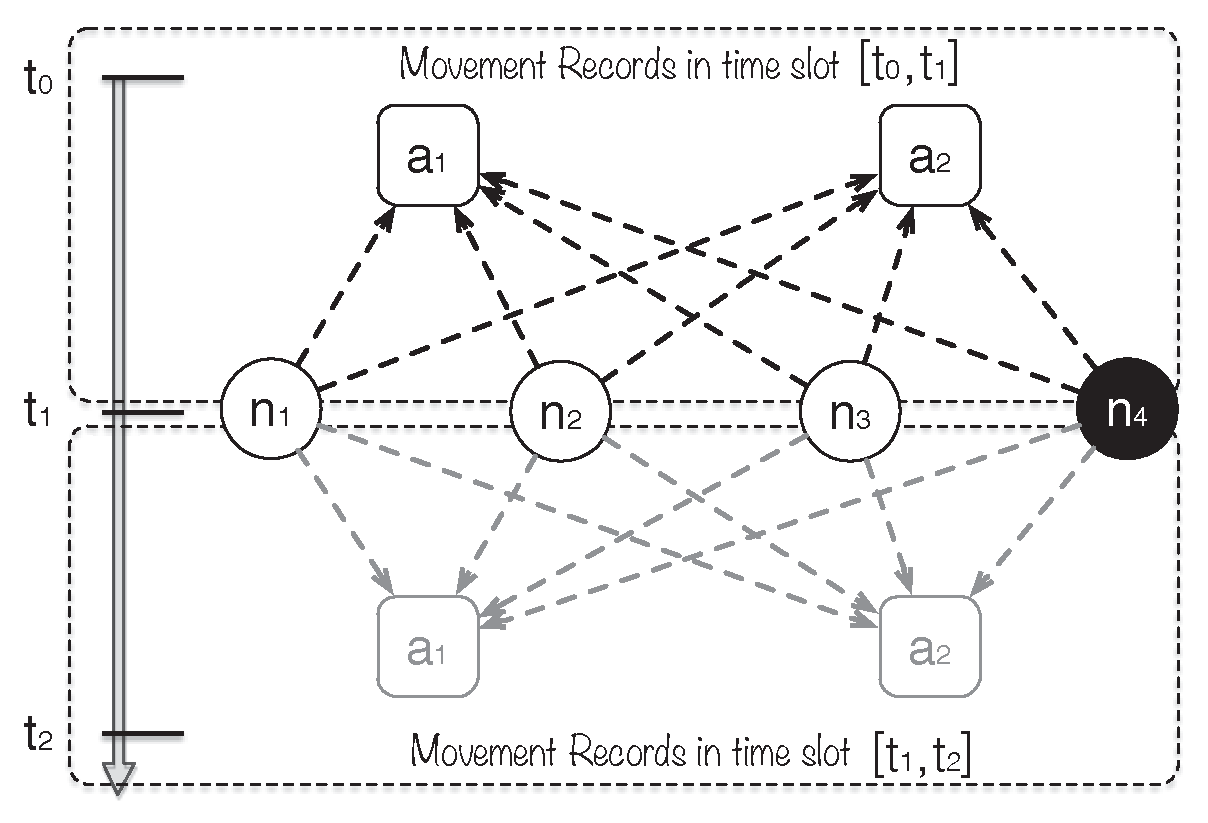
\includegraphics[width=0.7\linewidth]{paper-MPAR/example1}
  \caption{网络场景举例}
  \label{fig:chap3_example1}
\end{figure}

\begin{definition} 函数$\mathbbm{E}$
\[\mathbbm{E}([x_1,x_2,\ldots,x_m])=[\varkappa _1,\varkappa _2,\ldots,\varkappa _m]\]\textnormal{其中}
\begin{equation}
\varkappa _j=\left\{
\begin{array}{cl}
 1 &x_j\geq\frac{\updelta}{m}\sum_{i=1}^{i=m}x_i\\
 0 & otherwise
\end{array}
\right.
\label{eq:extract}
\end{equation}
\textnormal{$0<\updelta<1$ 是预设的系统参数。}
\label{def:函数E}
\end{definition}

函数$\mathbbm{E}$用于过滤节点—地点间的访问记录,不常访问的地点将被过滤掉。基于函数$\mathbbm{E}$可以直接定义移动模式,如定义\ref{def:移动模式}。

\begin{definition} 移动模式.
对于任意节点群组$N$,其在时间区间$[t_p,t_q]$ 内的移动模式,记为$\mathcal{P}(V,[t_s,t_e])$, 定义为
\begin{equation}
\mathcal{P}(N,[t_s,t_e])= \mathbbm{E}(\sum_{n_x \in N}\sum_{i=s}^{i=e}\mathbb{R}(x,t_i))
\label{eq:pattern}
\end{equation}
\label{def:移动模式}
\end{definition}

在定义\ref{def:移动模式}中,移动模式$\mathcal{P}$从某节点(群组)在某个特定时间区间$[t_s,t_e]$上的所有移动记录向量通过累加后,以函数$\mathbbm{E}$处理后得出。举例而言,假设如\figurename~\ref{fig:chap3_example1}所示的网络场景,网络中总共有四个节点$n_1,n_2,n_3,n_4$以及两个地点$a_1,a_2$。其中$n_4$是目的节点,周期$T$被划分为两个时间槽,简记为$[t_0,t_1]$与$[t_1,t_2]$。



\figurename~\ref{fig:chap3_example1}中每条边的权值如\tablename~\ref{tab:chap3_example1}所示。权值代表“节点—地点”对访问平均间隔时间。针对每个节点的记录矩阵,表示为$\mathbb{R}(1),\mathbb{R}(2),\mathbb{R}(3),\mathbb{R}(4)$。

\[
\begin{array}{cc}
\mathbb{R}(1)=\left[
\begin{array}{cc}
\sfrac{1}{2.08} & \sfrac{1}{4.65} \\
\sfrac{1}{6.02} & \sfrac{1}{2.95}
\end{array}\right]&
\mathbb{R}(2)=\left[
\begin{array}{cc}
\sfrac{1}{4.4} & \sfrac{1}{4.3} \\
\sfrac{1}{4.0} & \sfrac{1}{4.5}
\end{array}\right]    \\ \\
\mathbb{R}(3)=\left[
\begin{array}{cc}
\sfrac{1}{8.05} & \sfrac{1}{1.11} \\
\sfrac{1}{6.05} & \sfrac{1}{15.49}
\end{array}\right]
&
\mathbb{R}(4)=\left[
\begin{array}{cc}
\sfrac{1}{2.6} & \sfrac{1}{3.3} \\
\sfrac{1}{3.5} & \sfrac{1}{3.5}
\end{array}\right]
\end{array}
\]

\begin{table}[hbt]
\centering
  \caption{网络场景\figurename~\ref{fig:chap3_example1}边权值}
  \begin{tabular}{|c|c|cc|}
  \hline
    & & $a_1$ & $a_2$  \\
    \hline
    
    %%t1
    \multicolumn{1}{|c|}{\multirow{4}{*}{$[t_0,t_1]$}} & $n_1$ &2.08 & 4.65 \\
    & $n_2$ & 4.4 & 4.3 \\
    & $n_3$ & 8.05 & 1.11 \\
    & $n_4$ & 2.6 & 3.3 \\
    \hline

    %%t2
    \multicolumn{1}{|c|}{\multirow{4}{*}{$[t_1,t_2]$}} & $n_1$ &6.02 & 2.95 \\
    & $n_2$ & 4.0 & 4.5 \\
    & $n_3$ & 6.05 & 15.49 \\
    & $n_4$ & 3.5 & 3.5 \\
    \hline
  \end{tabular}
  \label{tab:chap3_example1}
\end{table}
节点集合$\{n_1,n_2,n_3\}$的移动模式,可以利用公式\ref{eq:pattern}从对应的移动记录中提取出来。对应的移动记录累加计算如下:
\begin{multline*}
\sum_{i=1}^{i=3}\sum_{j=1}^{j=2}\mathbb{R}(i,j) = \left[\frac{1}{2.08}+\frac{1}{4.4}+\frac{1}{8.05}+\frac{1}{6.02}+\frac{1}{4.0}+\frac{1}{6.05},\right.\\
\left.\frac{1}{4.65}+\frac{1}{4.3}+\frac{1}{1.11}+\frac{1}{2.95}+\frac{1}{4.5}+\frac{1}{15.49}\right]= [1.414,1.974]
\end{multline*}
针对公式\ref{eq:extract},设定参数$\delta=0.95$,从定义\ref{def:函数E}得出
\[
\frac{\updelta}{m}\sum_{i=1}^{i=m}v_i=\frac{0.95}{2}\times(1.414+1.974)\approx 1.609
\] 
所得值1.609大于向量第一个元素值1.414,且小于向量第二个元素值1.974,故对应移动模式提取如下
\[
\mathcal{P}(\{n_1,n_2,n_3\},[t_0,t_2])=[0,1] 
\]

移动模式$\mathcal{P}$指明了节点群组$\{n_1,n_2,n_3\}$在时间区间$[t_0,t_2]$内的的常访区域集合,即$A(\{n_1,n_2,n_3\},[t_0,t_2])=\{a_2\}$。对于集合$\overline{N}\\\{n_d\}$,共有$2^{n-1}-1$个非空子集,每一个子集可被看做用于向目的节点$n_d$合作投递消息的一个整体。在本例中,基于移动记录,提取出非空节点集$\{n_1,n_2,n_3\}$以及目的节点$n_4$的移动模式,结果如下\\
\begin{center}
\begin{tabular}{ll}
 & \\
$\mathcal{P}(\{n_1\},[t_0,t_2])=[1,0]$ & $\mathcal{P}(\{n_1,n_2\},[t_0,t_2])=[1,0]$ \\
$\mathcal{P}(\{n_2\},[t_0,t_2])=[1,1]$ & $\mathcal{P}(\{n_1,n_3\},[t_0,t_2])=[0,1]$ \\
$\mathcal{P}(\{n_3\},[t_0,t_2])=[0,1]$ & $\mathcal{P}(\{n_2,n_3\},[t_0,t_2])=[0,1]$ \\
$\mathcal{P}(\{n_4\},[t_0,t_2])=[1,1]$ & $\mathcal{P}(\{n_1,n_2,n_3\},[t_0,t_2])=[0,1]$ \\
 &
\end{tabular}
\end{center}
对应的常访地点集合,如下
\begin{center}
\begin{tabular}{ll}
 & \\
$A(\{n_1\},[t_0,t_2])=\{a_1\}$ & $A(\{n_1,n_2\},[t_0,t_2])=\{a_1\}$ \\
$A(\{n_2\},[t_0,t_2])=\{a_1,a_2\}$ & $A(\{n_1,n_3\},[t_0,t_2])=\{a_2\}$ \\
$A(\{n_3\},[t_0,t_2])=\{a_2\}$ & $A(\{n_2,n_3\},[t_0,t_2])=\{a_2\}$ \\
$A(\{n_4\},[t_0,t_2])=\{a_2\}$ & $A(\{n_1,n_2,n_3\},[t_0,t_2])=\{a_1,a_2\}$ \\
 &
\end{tabular}
\end{center}
\subsection{路由相关的两个关键属性}
\label{chap3:路由相关的两个关键属性}

\subsubsection{投递概率}

设节点集合$N$在时间区间$[t_0,t_0+t_l]$内的移动模式为$P(N,[t_0,t_0+t_l])$,目的节点$n_d$的移动模式为$\mathcal{P}(n_d,[t_0,t_0+\tau_l])$,共同常访地点集合记为$A$,则有$A=A(N,[t_0,t_0+\tau_l])\cap A(n_d,[t_0,t_0+\tau_l])$。记任意地点$a_j$及任意节点$n_i\in N$满足节点$n_i$和$n_d$
都在某一时间访问$a_j$。设随机变量$T_{i,j}$及$T_{d,j}$分别代表$n_i$和$n_d$到达$a_j$的时间,若要使消息能够成功传递,则须满足$T_{i,j}<T_{d,j}<\tau_l$,换言之,$n_i$须先于$n_d$到达$a_j$托管消息,且$n_d$需在消息到期之前到达$a_j$取出消息。为了便于讨论,设起始时间点$t_0=0$。此外,如\ref{chap3:系统模型及基本定义}节所述,任意节点访问任意地点的时间间隔服从指数分布。从公式\ref{eq:meeting_interval}可以计算出节点$n_i$访问地点$a_j$的指数分布参数$\lambda_{i,j}$,即

\[
\lambda_{i,j} = \sfrac{1}{M_{i,j}}
\]

对于$A$为空集的情形,默认其预测投递概率为0,到达其它地点的期望时延为$\infty$。对于$A$非空的情形,可依公式(\ref{eq:probability})预测节点$n_i$对$n_d$的投递率。进一步的,节点集$N$对$n_d$的投递率可依公式(\ref{eq:probability2})预测。
\begin{multline}
P_{i,d}=1-\prod_{a_j\in A}\left(1-P(T_{i,j}<T_{d,j}<\tau_l) \right) \\
=1-\prod_{a_j\in A}\left(1-\int _{0}^{\tau _l}\!\!\!\!\int _{t_{i,j}}^{\tau _l}f_{T_{i,j},T_{d,j}}\left(t_{i,j},t_{d,j}\right)dt_{d,j}dt_{i,j}\right)\\
=1-\prod_{a_j\in A}\left(1-\int _{0}^{\tau _l}\!\!\!\!\int _{t_{i,j}}^{\tau _l}f_{T_{i,j}}(t_{i,j})f_{T_{d,j}}(t_{d,j}) dt_{d,j}dt_{i,j}\right) \\
=1-\prod_{a_j\in A}\left(1-\int _{0}^{\tau _l}\!\!\!\!\int _{t_{i,j}}^{\tau _l}\lambda _{d,j} \lambda _{i,j} e^{-\left(\lambda _{d,j}t_{d,j}+\lambda _{i,j}t_{i,j}\right)}dt_{d,j}dt_{i,j}\right)\\
=1-\prod_{a_j\in A}\left(1-\frac{\lambda _{i,j} \left(1-e^{-\tau _l \left(\lambda _{d,j}+\lambda _{i,j}\right)}\right)}{\lambda _{d,j}+\lambda _{i,j}}
-\left(e^{\tau _l \lambda _{i,j}}-1\right) e^{-\tau _l \left(\lambda _{d,j}+\lambda _{i,j}\right)}\right)
\label{eq:probability}
\end{multline}
\begin{multline}
P_{N,d}=1-\prod_{n_i\in N}(1-P_{i,d}) \\
=1-\prod_{n_i\in N}\prod_{a_j\in A}\left(1-\frac{\lambda _{i,j} \left(1-e^{-\tau _l \left(\lambda _{d,j}+\lambda _{i,j}\right)}\right)}{\lambda _{d,j}+\lambda _{i,j}}
-\left(e^{\tau _l \lambda _{i,j}}-1\right) e^{-\tau _l \left(\lambda _{d,j}+\lambda _{i,j}\right)}\right)
\label{eq:probability2}
\end{multline}
特别而言,当消息生存时间设为无穷时,即$\tau_l=\infty$,有
\begin{multline}
P_{i,d} = 1-
\prod_{a_j\in A}\left(1-\int _0^{\infty }\!\!\!\!\int _{t_{i,j}}^{\infty }\lambda _{d,j} \lambda _{i,j} e^{-\left(\lambda _{d,j} t_{d,j}+\lambda _{i,j} t_{i,j}\right)}dt_{d,j}dt_{i,j} \right)\\
=1-\prod_{a_j\in A}\left(1-\frac{\lambda _{i,j}}{\lambda _{d,j}+\lambda _{i,j}}\right)
\label{eq:probability_infty}
\end{multline}
对于$P_{N,d}$,有
\begin{equation}
P_{N,d} = 1-\prod_{n_i\in N}\prod_{a_j\in A}\left(1-\frac{\lambda _{i,j}}{\lambda _{d,j}+\lambda _{i,j}}\right) 
=1-\prod_{n_i\in N}\prod_{a_j\in A}\frac{\lambda _{d,j}}{\lambda _{d,j}+\lambda _{i,j}}
\label{eq:probability2_infty}
\end{equation}

对于\figurename~\ref{fig:chap3_example1}中的例子,为简便起见,讨论$\tau_l=\infty$的情况(形式化定义时,会给出一般情况下的定义)。对于节点集合$\{n_1,n_2,n_3\}$而言,常访地点集合$A(N,[t_0,t_3])=\{a_2\}$;对于目的节点$n_d$而言,其常访地点集合$A(n_4,[t_0,t_3])=\{a_1,a_2\}$;由此可得出共同常访地点$A=\{a_2\}$。每一个“节点—地点”对的平均访问时间间隔,可从公式(\ref{eq:meeting_interval})获得,即

\[
\begin{array}{llll}
M_{1,1}=4.05 & M_{2,1}=4.2 & M_{3,1}=7.05 & M_{4,1}=3.05 \\
M_{1,2}=3.8 & M_{2,2}=4.4 & M_{3,2}=8.3 & M_{4,2}=3.4
\end{array}
\]

由以上计算结果,可预测节点集合$N$的投递概率,如下

\begin{multline*}
P_{\{n_1,n_2,n_3\},4}=
1-\left(\frac{\lambda_{4,2}}{\lambda_{1,2}+\lambda_{4,2}}\middle)\middle(\frac{\lambda_{4,2}}{\lambda_{2,2}+\lambda_{4,2}}\middle)\middle(\frac{\lambda_{4,2}}{\lambda_{3,2}+\lambda_{4,2}}\right) \\
= 1-\left(\frac{M_{1,2}}{M_{1,2}+M_{4,2}}\middle)\middle(\frac{M_{2,2}}{M_{2,2}+M_{4,2}}\middle)\middle(\frac{M_{3,2}}{M_{3,2}+M_{4,2}}\right) 
= 0.789
\end{multline*}

\subsubsection{期望时延}

除了投递概率之外,另一个关键的属性即节点移动到其他地点的期望时延。设节点$n_i$的常访地点集合为$A_i$,用随机变量$D_i$代表$n_i$移动到下一个地点$a_j\in A_i$的期望时延。形式上,有$D_i=\min\{T_{i,1},T_{i,2},\ldots,T_{i,|A_i|}\}$,由此可求得$D_i$的概率密度函数为
\[f_{D_i}(t)=\sum_{a_k\in A_i}\lambda_{i,k}\prod_{a_h\in A_i}e^{-\lambda_{i,h}t}\]
于是有
\begin{multline}
E[D_i]=\int_{-\infty}^{\infty}tf_{D_i}(t)dt 
=\sum_{a_k\in A_i}\int_{0}^{\infty}t\lambda_{i,k}\prod_{a_h\in A_i}e^{-\lambda_{i,h}t}dt \\
=\sum_{a_k\in A_i}\frac{\lambda_{i,k}}{\left(\sum_{a_k\in A_i}\lambda_{i,h}\right)^2}
=\frac{1}{\sum_{a_k\in A_i}\lambda_{i,k}}
\label{eq:delay}
\end{multline}
对于\figurename~\ref{fig:chap3_example1}所示例子,可以分别对节点$n_1$, $n_2$及$n_3$根据公式(\ref{eq:delay})计算期望时延$E[D_i]$。
\[
\begin{array}{l}
E[D_1]=\sfrac{1}{\lambda_{1,1}}=M_{1,1}=4.05\\
E[D_2]=\frac{1}{\lambda_{2,1}+\lambda_{2,2}}=\frac{M_{2,1}M_{2,2}}{M_{2,1}+M_{2,2}}=2.15\\
E[D_3]=\sfrac{1}{\lambda_{3,2}}=M_{3,2}=8.3 
\end{array}
\]
对于任意一对节点$n_i$和$n_j$,若$E[D_i]<E[D_j]$,则从期望意义上讲,$n_i$到达下一个新地点的时间要早于$n_j$,这意味着$n_i$能够更早的将消息托管到新的投掷盒。在机会网络中多使用多拷贝策略进行路由,快速的向网络中传播足够数目的消息副本,对提升路由性能至关重要。期望时延$E[D]$是一个很好的衡量指标,应尽可能的利用$E[D]$较小的节点分发消息。在本章提出的基于局部搜索的路由算法Local-MPAR中,$E[D]$被用于衡量节点作为网络中唯一的活跃节点是否合适。在基于禁忌搜索的路由算法Tabu-MPAR中,$E[D]$被用作向网络中非对称喷洒消息副本的衡量指标。在\tablename~\ref{tab:chap3_example1}所示例子中,节点$n_2$最适合作为活跃节点,因为其期望时延$E[D]$最低,因此在期望意义上,$n_2$可以较早的将消息拷贝托管给其它地点的投掷盒。

\subsection{路由问题形式化定义}
\label{chap3:路由问题形式化定义}

机会网络中的路由问题,其优化目标可有多种。衡量路由算法性能的最主要的两个指标,即是消息投递率和平均端到端时延。尽管端到端时延在路由优化中被看做一项非常重要的指标,但路由的性能表现仍需要以可被接受的投递概率为基础。换言之,较高的投递概率是保证网络正常工作的基础。本章意图最大化消息的投递概率,进而提高路由性能表现。即寻找子集$N\subseteq\overline{N}$,从而使得$P_{N,d}\geq P_{N',d}$对于$\forall N'\subseteq\overline{N}$成立,其中$n_d$是消息的目的节点。

在\figurename~\ref{fig:chap3_example1}所示例子中,可依\ref{chap3:路由相关的两个关键属性}小节中公式(\ref{eq:probability2}),预测集合$\{n_1,n_2,n_3\}$所有非空子集的投递率,如下
\[
\begin{array}{ll}
P_{\{n_1\},4}=0.430 & P_{\{n_1,n_2\},4}=0.670  \\
P_{\{n_2\},4}=0.673 & P_{\{n_2,n_3\},4}=0.600  \\
P_{\{n_3\},4}=0.291 & P_{\{n_1,n_3\},4}=0.626  \\
P_{\{n_1,n_2,n_3\}}=0.789\\
\end{array}
\]

在本例中,最优集合即$\{n_1,n_2,n_3\}$。注意计算结果为估计投递率,并不直接与持有该消息的节点数目成正比。投递率$P_{N,d}$基于节点集合$N$,$N$在整个路由过程中被看做一个整体。对于某个$N'\subset N$而言,概率$P_{N,d}<P_{N',d}$是可能发生的。事实上,如\figurename~\ref{fig:chap3_example1}所示,对于集合$\{n_2,n_3\}$而言,其预测投递率低于集合$\{n_2\}$的预测投递率。如果忽略缓存限制和能耗资源,向整个网络中广播每条消息会获得最好的性能表现,因为在这种情况下增加中继节点的数目,可以提高消息的投递率(或者说至少不可能降低)。然而这种理想的情况在机会网络中往往并不存在。真实情况下,往往倾向于选择能够符合一定移动模式的最小节点群组,对消息进行投递。从例中可以看出,如果把持有该消息的所有节点视为一个整体,则其预测投递率被两项指标所影响:(1)节点集对应的移动模式,(2)节点集的大小。在正式定义路由问题之前,首先给出最优节点集合$N_{opt}$的定义。

\begin{definition} The optimal set $N_{opt}$\\
最优集合$N_{opt}$包含网络中的一组节点, 且有
\begin{displaymath}
N_{opt}= \min\{\mathrel{\mathop{\arg\max}\limits_{N\subseteq \overline{N}}}P_{N,d}\}
\end{displaymath}
\end{definition}

最优集合是能够取得最高预测投递率的最小集合,集合中的节点以合作的方式将消息传递给目的节点。基于此,可定义最优路由问题。

\begin{definition}$N_{opt}$搜索问题.\\
令$f(\mathbf{x})$代表目标函数, $g(\mathbf{x})$代表限制函数, 其中决策变量表示为$\mathbf{x}=\{x_1,x_2,\ldots,x_n\}$,有 
\begin{tabular}{l}
\parbox{\linewidth}{
\begin{multline*}
f(\mathbf{x})=\sum_{i=1}^{i=n}x_i\log\left(\prod_{a_j\in A}\left(1-\frac{\lambda _{i,j} \left(1-e^{-\tau _l \left(\lambda _{d,j}+\lambda _{i,j}\right)}\right)}{\lambda _{d,j}+\lambda _{i,j}}\right.-\left.\left(e^{\tau _l \lambda _{i,j}}-1\right) e^{-\tau _l \left(\lambda _{d,j}+\lambda _{i,j}\right)}\right)\right)
\end{multline*}
}
\end{tabular}
\[
g(\mathbf{x})=\left|\sum_{i=1}^{i=n}x_i\right|
\]
于是问题可以被形式化为如下
\[
\begin{array}{c}
\min f(\mathbf{x}) \\
s.t.\forall\mathbf{x'},~g(\mathbf{x'})-g(\mathbf{x})\geq 0, \\
\forall i,x_i\in \{0,1\}
\end{array} 
\]
当求出最优节点集合$\mathbf{x}_{opt}$时,有
\[
N_{opt}=\{n_i|x_i>0,1\leq i\leq n\}
\]
\label{def:N_opt}
\end{definition}

在上述定义中,存在一个$\bm{x}$与$N$之间的一对一映射。事实上,有$f(\bm{x})=\log(1-P_{N,d})$,其中$f(\bm{x})$与$P_{N,d}$成负相关。由此,$N_{opt}$搜索问题被形式化为最优化问题。

\section{$N_{opt}$搜索问题分析}
\label{chap3:搜索问题分析}

本节讨论$N_{opt}$问题的计算复杂性,并提出了一种启发式方法,以近似计算最优解。首先证明对于在线算法(online algorithm),对于算法输入序列中新加入的元素,能够很大程度改变目标函数的值。对于离线算法(offline algorithm),给出了$\mathcal{NP}$-hard性质证明。最后,本章提出基于禁忌搜索的启发式算法。

\subsection{计算复杂性证明}
在线算法可以分片处理输入序列。换言之,算法的输入是以一个序列方式随时间交付由算法本身处理的,而不同于离线算法,需要一次接受整个算法输入。对于$N_{opt}$,其在线算法的输入是网络中节点的移动记录,简单表示为$\mathbb{R}_{1},\mathbb{R}_{2},\ldots,\mathbb{R}_{q}$ (其中序列中的每个元素都是一个向量,例如对于在时间槽$t_i$的节点$n_x$可以有$\mathbb{R}_j=\mathbb{R}(x,t_i)$)。假设当前只有序列的前$1--k$个元素被输入算法。剩下的问题即探究当下一个新元素$\mathbb{R}_{k+1}$被加入网络时,会在多大程度上影响目标函数的值, 见定理~\ref{thm:online}

\begin{theorem}
对于$\forall k\in[1,z)$, 即使序列的前$1$---$k$部分已知,新加入的元素$\mathbb{R}_{k+1}$仍可能将移动模式改变为至少有一个元素不为0的任意向量。
\label{thm:online}
\end{theorem}
\begin{proof}
将任意向量$R_i$表示为如下
\[
R_i=[r^i_1,r^i_2,\ldots,r^i_m]~~~\forall j\in[1,m], r^i_j\geq 0
\]
向量$\sum_{i=1}^{i=k}\mathbb{R}_{i}$ 表示为
\[
\sum_{i=1}^{i=k}\mathbb{R}_{i}=[S^{k}_1,S^{k}_2,\ldots,S^{k}_m]
\]
于是对于$\forall i\in [1,m]$及 $k\in [1,z)$ 有
\[
S^{k+1}_i=S^{k}_i+r^{k+1}_i
\]
相应地,用 $\mathcal{P'}=\mathbbm{E}(\sum_{i=1}^{i=k+1}\mathbb{R}_{i})$ 和 $\mathcal{P}=\mathbbm{E}(\sum_{i=1}^{i=k+1}\mathbb{R}_{i})$ 分别表示在加入新元素$\mathbb{R}_{k+1}$之前和之后的移动模式向量。 现证明对于任意的$\mathcal{P}$, 都存在一个可能的新元素$\mathbb{R}_{k+1}$,能使向量$\mathcal{P'}$ 变为 $\mathcal{P}$.
当已知$\mathcal{P}=[\varkappa _1,\varkappa _2,\ldots,\varkappa _m]$时, 显然$\mathbb{R}_{k+1}$存在,当且仅当如下线性不等式组成立
\begin{displaymath}
\forall i\in[1,m]~~~~
\left\{
\begin{array}{ll}
S^{k+1}_i\geq\delta\sum_{j=1}^{j=m}\left(\sfrac{S^{k+1}_j}{m}\right)& \varkappa_i=1 \\
S^{k+1}_i<\delta\sum_{j=1}^{j=m}\left(\sfrac{S^{k+1}_j}{m}\right) & \varkappa_i=0
\end{array}
\right.
\end{displaymath}
即
\[
\left\{
\begin{array}{ll}
\sum_{j=1}^{j=m}r_j^{k+1}-\frac{m}{\delta}r_i^{k+1}\leq \frac{m}{\delta}S_i^{k}-\sum_{j=1}^{j=m}S_j^{k} & \varkappa_i=1 \\
\sum_{j=1}^{j=m}r_j^{k+1}-\frac{m}{\delta}r_i^{k+1}> \frac{m}{\delta}S_i^{k}-\sum_{j=1}^{j=m}S_j^{k} & \varkappa_i=0 \\
\end{array}\right.
\]

对于 $\forall i$, 将 $\frac{m}{\delta}S_i^{k}-\sum_{j=1}^{j=m}S_j^{k}$ 表示为 $w_i$, 并将$\varkappa_i=1$ 和 $\varkappa_i=0$ 时的$w_i$分别表示为 $w_{i|\varkappa_i=1}$ 和$w_{i|\varkappa_i=0}$。 同理,用 $r_i^{k+1}$ 表示 $\varkappa_i=1$ 和 $\varkappa_i=0$ 时的对应状态,有
\begin{equation}
\sum_{j=1}^{j=m}r_j^{k+1}-\frac{m}{\delta}r_{i|\varkappa_i=0}^{k+1}> w_{i|\varkappa_i=0}  
\label{eq:varkappa_0}
\end{equation}
且有
\begin{equation}
\sum_{j=1}^{j=m}r_j^{k+1}-\frac{m}{\delta}r_{i|\varkappa_i=1}^{k+1}\leq w_{i|\varkappa_i=1}
\label{eq:varkappa_1}
\end{equation}
令 $r^{k+1}_{i|\varkappa_i=0}=0$ 及 $\sum_{j=1}^{j=m}r_j^{k+1}=\max\{w_i\}+\epsilon~(\epsilon>0)$, 则等式(\ref{eq:varkappa_0})对于 $\forall \varkappa_i=0$都成立。

接下来证明可以选择足够大的$\epsilon$值,使得等式\ref{eq:varkappa_1}成立,即只需让 $\sum_{j=1}^{j=m}r_j^{k+1}-\frac{m}{\delta}r_{i|\varkappa_i=1}^{k+1}\leq \min\{w_i\}$ 对于 $\forall \varkappa_i=1$都成立,即
\[
\max\{w_i\}+\epsilon-\frac{m}{\delta}r_{i|\varkappa_i=1}^{k+1}\leq \min\{w_i\}
\]
从上述讨论, 只需让下述不等式同时成立.
\begin{equation}
r_{i|\varkappa_i=1}^{k+1}\geq\frac{\delta}{m}(\max\{w_i\}-\min\{w_i\}+1)~(0<\delta<1)
\label{eq:q1}
\end{equation}
\begin{equation}
\sum_{j=1}^{j=m}r_{j|\varkappa_j=1}^{k+1}=\max\{w_i\}+\epsilon
\label{eq:q2}
\end{equation}
假设$\mathcal{P}$中 $\varkappa_i=1$ 的数量是 $z$, 由于 $0<z\leq m$, 有
\[
z\cdot\frac{\delta}{m}(\max\{w_i\}-\min\{w_i\}+\epsilon) \leq  
\delta(\max\{w_i\}-\min\{w_i\}+\epsilon) 
\]
为使等式(\ref{eq:q1})和(\ref{eq:q2})同时成立, 只须有
\[
\delta(\max\{w_i\}-\min\{w_i\}+\epsilon) < \max\{w_i\}+\epsilon = \sum_{j=1}^{j=m}r_{j|\varkappa_j=1}^{k+1}
\]
即
\[
\epsilon>\frac{\delta}{\delta-1}\min\{w_i\}-\max\{w_i\}
\]
证毕
\end{proof}

定理~\ref{thm:npc}~给出$N_{opt}$计算复杂性的证明。

\begin{theorem}
$N_{opt}$问题属于$\mathcal{NP}$-hard类. 
\label{thm:npc}
\end{theorem}
\begin{proof}
%We reduce the $N_{opt}$ Search Problem as a Subset Sum Problem (SSP). Assume that we know a solution for a certain SSP instance of which all the elements are denoted by $R={r_1,r_2,\ldots,r_n}$ and the target value is $v$. For clarity, we transform $R$ as follows:
将子集和问题(Subset Sum Problem, SSP)归约为$N_{opt}$问题。假设已知SSP问题的一个解实例,用 $R={r_1,r_2,\ldots,r_n}$,目标值用$v$表示。为清楚起见,将$R$变为如下形式
\begin{displaymath}
R=\{\log 2^{r_1},\log 2^{r_2},\ldots,\log 2^{r_n}\}
=\{\log g_1,\log g_2,\ldots,\log g_n\}
\end{displaymath}
其中有 $g_i=2^{r_i}~~(i\in[1,n])$.
将其所有非空子集表示为 $R_1,R_2\ldots, R_{2^{|N|-1}}$。接下来,构造对应的 $N_{opt}$ 实例。 目标值为$P=v$, 节点集合为$N={n_1,n_2,\ldots,n_n}$, 对应上述提到的集合$R$. 对于每一个$N$的非空子集$N_i$, 都存在一个$R$的子集$R_i$与其一一对应 (所有的角标都是一一对应的), 将任意子集$N_j$表示为如下
\[
N_j=\{n_{j_1},n_{j_2},\ldots,n_{j_k}\}
\]
对于$\forall j$, 令$\lambda_{i,j}=1$, $\tau_{l}=\sqrt{2}$, 对于 $\forall n_i\in N-d$, 令$\lambda_{i,j}=\Lambda_i$. 此外, 令所有的节点都具有相同的移动记录$\mathbb{R}=[0,0,\ldots,0]$.于是,对于网络中所有的节点,都有
\[
\mathcal{P}=[1,1,\ldots,1]
\]

于是有
\[
P_{N_j,d}=1-\prod_{n_i\in N}(1-\Lambda_{i}e^{-\Lambda_i -1})^n
\]
令 $\kappa_i=\left(1-\Lambda_i e^{-\Lambda_i-1}\right)^{n}$, 则有
\[
P_{N_j,d}=1-\kappa_{j_1}\kappa_{j_2}\cdots\kappa_{j_k}
\]

由此,对于问题SSP的任意一个解实例,一定有一个问题$N_{opt}$ 的解实例与之对应。换言之
\[
v=\log (g_{j_1}g_{j_2}\cdots g_{j_k})\Longleftrightarrow P_{N_j,d}=1-\kappa_{j_1}\kappa_{j_2}\cdots\kappa_{j_n}
\]
反之, 若SSP问题无解, 则$N_{opt}$问题一定也无解. 因为若 $N_{opt}$ 有解, 则存在一个集合$R_j={r_{j_1},r_{j_2},\ldots,r_{j_n}}$ 使下式成立
\[
P=P_{N_j}
\]
与题设矛盾。\\
证毕
\end{proof}


\subsection{局部陷阱}

对于$N_{opt}$,一种直接的解法是局部搜索算法。然而,这有可能会陷入局部最优陷阱。对\figurename~\ref{fig:chap3_example1}中例子而言,假设节点$n_2$产生一条目的节点为$n_4$的消息,则其局部搜索过程如\tablename~\ref{tab:chap3_local_search}所示。

\begin{table}[hbt]
  \caption{\figurename~\ref{fig:chap3_example1}中的局部搜索过程示例}
  \centering
  \begin{tabular}{|c|c|c|c|c|c|c|}
    \hline
    %empty 
    & \multicolumn{3}{c|}{current solution}
    & \multicolumn{3}{c|}{next options}
    \\    
    \cline{2-7}
    
    %empty 
    & $\textbf{x}^{now}$ & N & $P_{N,4}$ & $\textbf{x}^{next}$ & N' & $P_{N',4}$ \\
    \hline
    
    %%%%step 1
    \multicolumn{1}{|c|}{\multirow{3}{*}{\textbf{Step 1}}}
    &\multicolumn{1}{c|}{\multirow{3}{*}{$[0,1,0]$}}
    &\multicolumn{1}{c|}{\multirow{3}{*}{$\{n_2\}$}}
    &\multicolumn{1}{c|}{\multirow{3}{*}{$0.673$}}
    &$[0,1,\underline{1}]$ &$\{n_2,n_3\}$ & $0.600$ 
    \\
    
    \multicolumn{1}{|c|}{}
    &\multicolumn{1}{c|}{}
    &\multicolumn{1}{c|}{}
     &\multicolumn{1}{c|}{}
    &$[0,\underline{0},0]$ & $\phi$ & $0$
    \\
    
    \multicolumn{1}{|c|}{}
    &\multicolumn{1}{c|}{}
    &\multicolumn{1}{c|}{}
        &\multicolumn{1}{c|}{}
    &$[\underline{1},1,0]$ & $\{n_1,n_2\}$ & $0.670$
    \\
    
    \hline
        %%%%stop
    \multicolumn{1}{|c|}{\multirow{3}{*}{\textbf{Stop}}}
    &\multicolumn{1}{c|}{\multirow{3}{*}{$[0,1,0]$}}
    &\multicolumn{1}{c|}{\multirow{3}{*}{$\{n_2\}$}}
    &\multicolumn{1}{c|}{\multirow{3}{*}{$0.673$}}
    &\multicolumn{1}{c|}{\multirow{3}{*}{---}} 
    &\multicolumn{1}{c|}{\multirow{3}{*}{---}}  
    &\multicolumn{1}{c|}{\multirow{3}{*}{---}}   
    \\
    
    \multicolumn{1}{|c|}{}
    &\multicolumn{1}{c|}{}
    &\multicolumn{1}{c|}{}
     &\multicolumn{1}{c|}{}
    & &  & 
    \\
    
    \multicolumn{1}{|c|}{}
    &\multicolumn{1}{c|}{}
    &\multicolumn{1}{c|}{}
        &\multicolumn{1}{c|}{}
    & &  & 
    \\
    \hline    
  \end{tabular} 
  \label{tab:chap3_local_search}
\end{table}

如\figurename~\ref{tab:chap3_local_search},在开始时只有节点$n_2$持有该消息,对于$N=\{n_2\}$,其预测投递率为$0.673$,高于其周围i任何一个可行解所对应的目标值。算法会误认为当前解$\bm{x}^{now}$即是最优解,然而真正的最优解是$[1,1,1]$,对应预测投递率$0.789$。在本例中,算法掉入了局部最优陷阱,而局部搜索算法无法跳出该陷阱。

\subsection{基于禁忌搜索的求解方法}

本小节基于禁忌搜索,提出解决$N_{opt}$的启发式算法,框架见算法~\ref{alg:chap3_framework}所示。

\begin{algorithm}[!tbp] %算法的开始
\renewcommand{\algorithmicensure}{\textbf{Step}}
\caption{Tabu Search Framework.} %算法的标题
\label{alg:chap3_framework} %给算法一个标签,这样方便在文中对算法的引用
\begin{algorithmic}[1] %这个1 表示每一行都显示数字
\REQUIRE ~\\
\begin{center}
\begin{tabular}{|c|c|}
\hline
\textbf{notation} & \textbf{meaning}\\
\hline
$p$ & Evaluation function\\
$\mathcal{N}$ & Neighborhood of a solution\\
$\mathcal{S}$ & Solution space\\
$\mathcal{E}$ & Stop rules \\
$\mathcal{T}$ & tabu table $\left\{\begin{tabular}{c|c} 
               $\varphi$ & Tabu element \\
               \hline
               $\mathcal{L}$ & Tabu length\\
                \end{tabular}\right.$\\
$\mathcal{A}$ & Aspiration criteria\\
\hline
\end{tabular}
\end{center}
\end{algorithmic} %这个1 表示每一行都显示数字
\begin{algorithmic}[1] %这个1 表示每一行都显示数字
\ENSURE \textbf{1:}
\STATE choose an initial feasible solution $\textbf{x}^{now}$ in $\mathcal{S}$
\STATE set the current best solution $\textbf{x}^{best}\leftarrow\textbf{x}^{now}$
\STATE set the tabu table $\mathcal{T}\leftarrow\emptyset$
\end{algorithmic} %这个1 表示每一行都显示数字
\begin{algorithmic}[1] %这个1 表示每一行都显示数字
\ENSURE \textbf{2:}
\IF{$\mathcal{E}(\textbf{x}^{best})=\textbf{true}$}
    \RETURN $\textbf{x}^{best}$
\ENDIF
\STATE get $C$ by filtering $\mathcal{N}(\textbf{x}^{now})$ according to $\mathcal{T}$ and $\mathcal{A}$
%location 1
\STATE $\textbf{x}^{now}\leftarrow\mathrel{\mathop{\arg\max}\limits_{\textbf{x}\in C}}p(\textbf{x})$
\IF{$p(\textbf{x}^{now})<p(\textbf{x}^{best})$}
    \STATE $\textbf{x}^{best}\leftarrow\textbf{x}^{now}$
\ENDIF
\STATE update $\mathcal{T}$
\STATE \textbf{goto} Step 2
\end{algorithmic}
\end{algorithm}

禁忌搜索过程可被分为两步,即Step 1和Step 2,其基本规则和数据结构见算法~\ref{alg:chap3_framework}内的表格。其中数学符号的正式定义将在下文给出。整个搜索过程即是在解空间中一步一步更改当前可行解,同时评估该可行解对应的目标函数值,从而尝试获得最优解。Step 1是禁忌搜索的初始化步骤,其中算法将在解空间$S$中选择一个可行解作为当前解,记为$\bm{x}^{now}$。接着,最优解也被初始化为$\bm{x}^{now}$,在此时,禁忌表$\mathcal{T}$中并无记录,如Step 1中行3所示。

在Step 2中,若停止规则$\mathcal{E}$被满足,则搜索过程终止并返回当前最优解$\bm{x}^{best}$作为最终结果。若不满足停止规则,则从$\bm{x}^{now}$的所有邻居$\mathcal{N}(\bm{x}^{now})$中选择一个可行解更新$\bm{x}^{now}$,该选择过程参照禁忌表$\mathcal{T}$的状态,以及预先定义的特赦准则$\mathcal{A}$。接着,算法将搜索子集$C$,并选择能够使函数$p$取得最大值的$\bm{x}$解向量。在Step 2的每一轮迭代中,都会尝试更新最优解$\bm{x}^{best}$。最终,禁忌表$\mathcal{T}$中对应的禁忌元素$\phi$将会被更新为预先定义的禁忌步长$\mathcal{L}(\phi)$。

下面给出算法\ref{alg:chap3_framework}中所有数学符号的定义。

\begin{definition}评估函数.\\
禁忌搜索中的评估函数表示为$p(\textbf{x})$, 有
\[
p(\textbf{x})=-f(\textbf{x})
\]
\label{def:eva_func}
\end{definition}

在定义~\ref{def:eva_func}中,评估函数设为对定义~\ref{def:N_opt}中函数$f(\bm{x})$的值取反。于是,搜索算法的目标即最大化评估函数的值。对于任一可行解向量$\bm{x}$,规定其邻域如定义~\ref{def:neighborhood}

\begin{definition}邻域.\\
令 $\textbf{x}=[x_1,x_2,\ldots,x_n]$$(\forall i, x_i\in{0,1})$ 为任一可行解向量, 则在算法中$\textbf{x}$的邻域$\mathcal{N}(\bm{x})$定义如下
\begin{equation}
\mathcal{N}(\textbf{x})=\left\{~\textbf{x'}~\middle|~~\sum_{i=1}^{n}\left| x_i- x'_j\right|\leq 1\right\}
\end{equation}
\label{def:neighborhood}
\end{definition}

如定义~\ref{def:neighborhood},某可行解的领域中的任一元素,与该可行解在向量上只有一个元素的差距。例如,如果当前可行解$\bm{x}$为$[0,1,0,1]$,则其邻域
\[
\mathcal{N}(\textbf{x})=\{[\underline{1},1,0,1],[0,\underline{0},0,1],[0,1,\underline{1},1],[0,1,0,\underline{0}]\}
\]
其中每一个向量都是$\bm{x}$的相邻解向量,下划线位置即是对原向量对应位置“取反”得到。事实上,整个解空间可被看做一个超立方体,其中每个顶点对应一个可行解向量,且解的邻域对应其在超立方体中的所有邻居节点,如\figurename~\ref{fig:chap3_hypercube}所示。

\begin{figure}[!t]
\centering
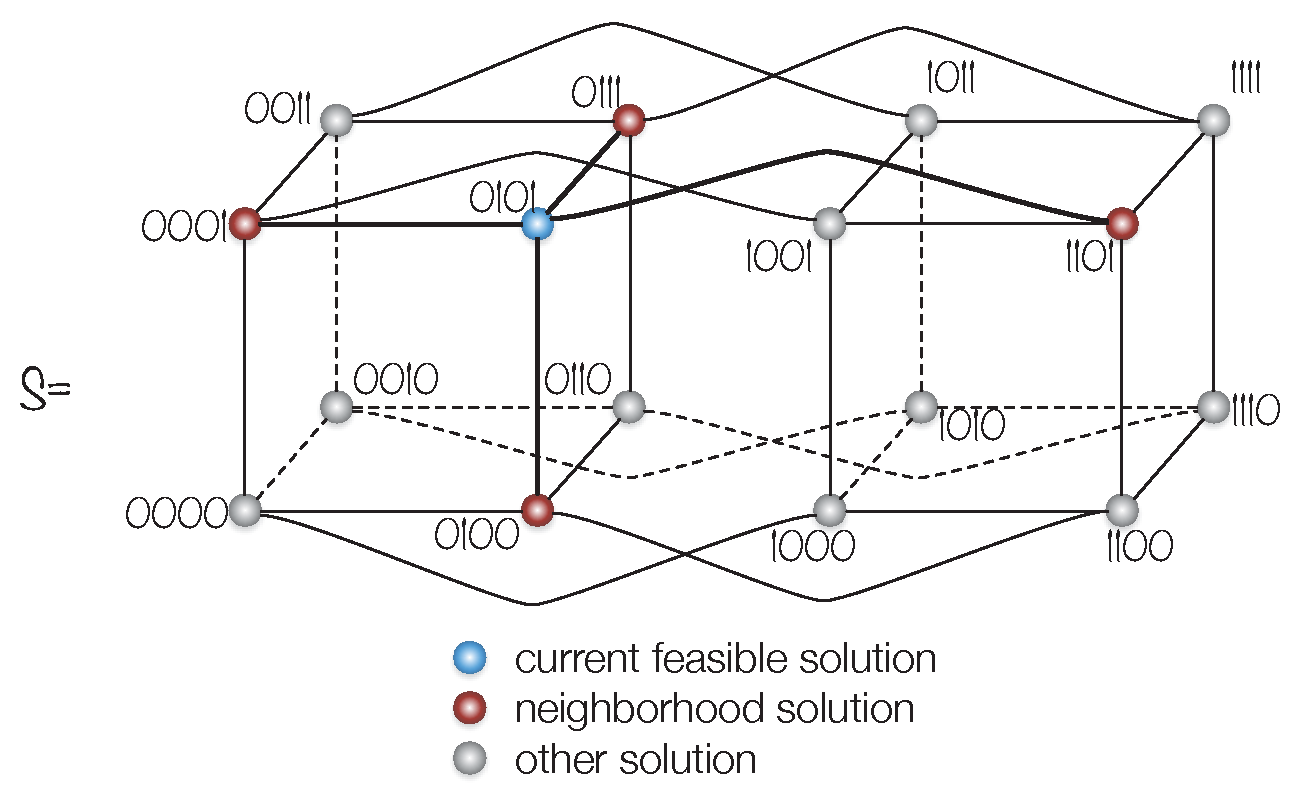
\includegraphics[width=4.0in]{paper-MPAR/hypercube}
\caption{超立方体解空间}
\label{fig:chap3_hypercube}
\end{figure}

停止规则是禁忌搜索中最重要的准则之一,其决定搜索过程停止的条件。在本算法中,停止规则如定义~\ref{def:stop_rule}所示。

\begin{definition}停止规则\\
停止规则 $\mathcal{E}$ 如下定义
\[
\mathcal{E}(\textbf{x}^{best})=\left\{
\begin{array}{cl}
true & \textnormal{if $p(\textbf{x}^{best})$ not improved after $\theta$ steps} \\
false & \textnormal{otherwise}
\end{array}\right.
\]
\label{def:stop_rule}
\end{definition}

如之前所述,评估函数$p$的值在搜索过程的每一次迭代中都被更新。如果当前解向量$\bm{x}^{now}$对应更好的评估函数值,即若有$p(\bm{x}^{now})>p(\bm{x}^{best})$,则用$\bm{x}^{now}$的值更新$\bm{x}^{best}$。然而,若当前记录的最优解对应的评估函数值$p(\bm{x}^{best})$在一定步数之内都未被更新,则意味着算法可能无法找到更好的解(在算法本身不被修改的前提下)。在这种情况下,搜索过程停止,当前最优解向量将作为返回值从算法返回。

禁忌表$\mathcal{T}$由两个主要元素组成,禁忌对象$\phi$和禁忌长度$\mathcal{L}(\phi)$。禁忌对象是禁忌搜索算法中实施禁忌的目标元素,可以定义为解向量的变化,或评估函数的变化。在本算法中,禁忌对象见定义~\ref{def:tabu_element}。

\begin{definition}禁忌对象\\
禁忌对象为解向量的变化,形式化定义如下
\[
\varphi:\textbf{x}\rightarrow\textbf{x'}
\]
有
\[
\textbf{x}=(x_1,\ldots,x_{i-1},x_i,x_{i+1},\ldots,x_n)~~(i\in [0,n])
\]
且
\[
\textbf{x'}=(x_1,\ldots,x_{i-1},y_i,x_{i+1},\ldots,x_n)~~(i\in [0,n], x_i\neq y_i)
\]
\label{def:tabu_element}
\end{definition}

事实上,禁忌对象是当前解向量在超立方体中对应的顶点向邻接顶点的迁移。正如\figurename~\ref{fig:chap3_hypercube}所示,从蓝色顶点(当前解)向红色顶点的迁移,即为禁忌对象。禁忌表中的禁忌长度如定义~\ref{def:tabu_length}。

\begin{definition}禁忌长度\\
禁忌长度由$\mathcal{L}(\varphi)$表示, 有
\[
\mathcal{L}(\varphi)=\lfloor T\rfloor
\]
T是服从正态分布的随机变量,有$T\sim N(\mu,\sigma^2)$, 且令
\[
\mu=\left\{
\begin{array}{ll}
\sqrt{n}[1+p(\textbf{x'})-p(\textbf{x})] & p(\textbf{x'})>p(\textbf{x}) \\
\sqrt{n} & \textnormal{otherwise}
\end{array}
\right.
\]
\label{def:tabu_length}
\end{definition}

在定义~\ref{def:tabu_element}中,禁忌长度设为对服从正态分布的随机变量$T$做下取整,其中正态分布的参数$\mu$保证了对于能让目标函数值变的更好的解向量,在统计意义上具有一个较长的禁忌长度。将禁忌长度设为一个随机数,而非常量,其意义在于向搜索算法中加上一定的随机因素,如同舍伍德算法一样。随机性能够帮助算法跳出一些无休止的循环,且能在算法输入被蓄意设定的情况下表现的更好。对于禁忌长度,值$T$与评估函数的变化程度$|p(\bm{x})-p(\bm{x'})|$具有一定关系。评估函数值发生变化具有两种情况;第一种情况下$p(\bm{x'})<p(\bm{x})$,意味着评估函数值到达了一个新的“山谷”;第二种情况下$p(\bm{x'})>p(\bm{x})$,意味着评估函数值爬上了一个比以往更高的“峰顶”。在第一种情况下,应将禁忌长度设的更大,从而让算法能够跳出当前的局部陷阱;对于第二种情况,应将禁忌长度设的更小,以免解向量移动的太远,再次掉入另一个“山谷”。定义~\ref{def:tabu_element}中的设定正好符合以上几点,此外对于正态分布参数$\mu$,有$\mu\in[\sqrt{n},2\sqrt{n}]$。

从定义~\ref{def:tabu_element}和定义~\ref{def:tabu_length}出发,算法禁忌表见定义~\ref{def:tabu_table}。

\begin{definition}禁忌表\\
禁忌表的结构如下 \\
\begin{center}
$\mathcal{T}$=
  \begin{tabular}{|c|c|cc|c|c|}
  \hline
   $1$ & $2$ & $\cdots$ & $\cdots$ & $n-1$ & $n$\\
   \hline
   $t_1$ & $t_2$ & $\cdots$ & $\cdots$ & $t_{n-1}$ & $t_n$ \\
    \hline
  \end{tabular} \\
\end{center}
假设禁忌对象为 $\varphi:\textbf{x}->\textbf{x'}$, 其更新规则如下
\[
\forall i, t_i=\left\{
\begin{array}{ll}
\mathcal{L}(\varphi) & \textnormal{if $|x_i-x'_i|=1$} \\
  0 & \textnormal{if}~t_i=0 \\
t_i-1 &  \textnormal{otherwise} \\
\end{array}
\right.
\]
\label{def:tabu_table}
\end{definition}

禁忌表$\mathcal{T}$设为一个$2\times n$的表,其中第一行代表禁忌对象中解向量的变化位置,第二行代表对于每个位置当前的禁忌步长。例如,设当前解向量发生变化,其对应的禁忌对象为$\phi:[0,1,0]\rightarrow[1,1,0]$,则应当按如下更新当前的禁忌表(其中$t_1,t_2,t_3>0$)
\begin{center}
\begin{tabular}{|c|c|c|}
\hline
1 & 2 & 3 \\
\hline
$t_1$ & $t_2$ & $t_3$ \\
\hline
\end{tabular} $\longrightarrow$
\begin{tabular}{|c|c|c|}
\hline
1 & 2 & 3 \\
\hline
$\mathcal{L}(\varphi)$ & $t_2-1$ & $t_3-1$ \\
\hline
\end{tabular}
\end{center}
对于算法的每一次更新操作,向量变化所对应的位置,在禁忌表中都会以$\mathcal{L}(\phi)$值更新,其它所有非零的表格元素都会做减1操作。任意位置,若其对应的禁忌步长不为0,则仅当禁忌步长降为0时,当前解向量才可从该位置向对应的相邻解向量迁移。

禁忌搜索中另一个重要的法则,即为特赦准则。特赦准则可以对禁忌表中特定的禁忌对象进行赦免,从而使其能被算法重新选取。特赦准则如定义~\ref{def:aspiration}

\begin{definition} 特赦准则\\
特赦准则如下定义
\begin{center}
\begin{tabular}{|c|}
\hline
对于 $\forall\bm{x}$, 若有 $p(\textbf{x})>p(\textbf{x}^{best})$ \\
则解向量 $\textbf{x}$ 可以作为下一步选择,即使其在禁忌表$\mathcal{T}$中被禁 \\
\hline
\end{tabular}
\end{center}
\label{def:aspiration}
\end{definition}

当所有的位置都在表$\mathcal{T}$中被禁时,当前解向量无法迁移到任何一个邻居向量。然而当某一个邻居向量所对应的评估函数值,优于当前所记录的最优值,则该向量会以特赦准则被解禁,即可以被算法选取。

\figurename~\ref{fig:chap3_example1}所示例子所对应的禁忌搜索过程,如\figurename~\ref{tab:chap3_tabu_search}。如同\tablename~\ref{tab:chap3_local_search}所示的局部搜索一样,消息源节点依然被选为$n_2$,且初始解向量为$[0,1,0]$。为了简化表述,在此,禁忌表长$\mathcal{L}$设定为常数$3$,而非定义中所述的随机量。此外,定义~\ref{def:stop_rule}中的$\theta$值设为$3$.

\begin{table*}[hbt]
  \caption{\figurename~\ref{fig:chap3_example1}例子对应的禁忌搜索过程}
  \resizebox{\textwidth}{!}{
  \begin{tabular}{|c|c|c|c|c|c|c|c|c|c|c|c|}
    \hline
    %empty 
    & \multicolumn{3}{c|}{current solution}
    & \multicolumn{3}{c|}{current best solution}
    & \multicolumn{1}{c|}{\multirow{2}{*}{tabu table $\mathcal{T}$}}
    & \multicolumn{4}{c|}{next options}
    \\    
    \cline{2-7}\cline{9-12}
    
    %empty 
    & $\textbf{x}^{now}$ & N & $P_{N,4}$ & $\textbf{x}^{best}$ & $N^{best}$ & $P_{N^{best},4}$ & & $\textbf{x}^{next}$ & N' & $P_{N',4}$ & status \\
    \hline
%    
    %%%%step 1
    \multicolumn{1}{|c|}{\multirow{3}{*}{\textbf{Step 1}}}
    &\multicolumn{1}{c|}{\multirow{3}{*}{$[0,1,0]$}}
    &\multicolumn{1}{c|}{\multirow{3}{*}{$\{n_2\}$}}
    &\multicolumn{1}{c|}{\multirow{3}{*}{$0.673$}}
    &\multicolumn{1}{c|}{\multirow{3}{*}{$[0,1,0]$}}
    &\multicolumn{1}{c|}{\multirow{3}{*}{$\{n_2\}$}}
    &\multicolumn{1}{c|}{\multirow{3}{*}{$0.673$}}
    &\multicolumn{1}{c|}{\multirow{3}{*}{$
                                                     \begin{tabular}{|c|c|c|}
                                                        \hline
                                                        1 & 2 & 3 \\
                                                        \hline
                                                        0 & 0 & 0 \\
                                                        \hline
                                                     \end{tabular}$}}
    &$[\underline{1},1,0]$ &$\{n_1,n_2\}$ & $0.670$ & choosable
    \\
    
    \multicolumn{1}{|c|}{}
    &\multicolumn{1}{c|}{}
    &\multicolumn{1}{c|}{}
    &\multicolumn{1}{c|}{}
    &\multicolumn{1}{c|}{}
    &\multicolumn{1}{c|}{}
    &\multicolumn{1}{c|}{}
    &\multicolumn{1}{c|}{}
    &$[0,\underline{0},0]$ & $\phi$ & $0$ & choosable
    \\
    
    \multicolumn{1}{|c|}{}
    &\multicolumn{1}{c|}{}
    &\multicolumn{1}{c|}{}
    &\multicolumn{1}{c|}{}
    &\multicolumn{1}{c|}{}
    &\multicolumn{1}{c|}{}
    &\multicolumn{1}{c|}{}
    &\multicolumn{1}{c|}{}
    &$[0,1,\underline{1}]$ & $\{n_2,n_3\}$ & $0.600$ & choosable
    \\
    \hline
    
    %%%%step 2
    \multicolumn{1}{|c|}{\multirow{3}{*}{\textbf{Step 2}}}
    &\multicolumn{1}{c|}{\multirow{3}{*}{$[1,1,0]$}}
    &\multicolumn{1}{c|}{\multirow{3}{*}{$\{n_1,n_2\}$}}
    &\multicolumn{1}{c|}{\multirow{3}{*}{$0.670$}}
    &\multicolumn{1}{c|}{\multirow{3}{*}{$[0,1,0]$}}
    &\multicolumn{1}{c|}{\multirow{3}{*}{$\{n_2\}$}}
    &\multicolumn{1}{c|}{\multirow{3}{*}{$0.673$}}
    &\multicolumn{1}{c|}{\multirow{3}{*}{$
                                                     \begin{tabular}{|c|c|c|}
                                                        \hline
                                                        1 & 2 & 3 \\
                                                        \hline
                                                        3 & 0 & 0 \\
                                                        \hline
                                                     \end{tabular}$}}
    &$[\underline{0},1,0]$ &$\{n_2\}$ & $0.673$ & tabu
    \\
    
    \multicolumn{1}{|c|}{}
    &\multicolumn{1}{c|}{}
    &\multicolumn{1}{c|}{}
    &\multicolumn{1}{c|}{}
    &\multicolumn{1}{c|}{}
    &\multicolumn{1}{c|}{}
    &\multicolumn{1}{c|}{}
    &\multicolumn{1}{c|}{}
    &$[0,\underline{0},0]$ & $\phi$ & $0$ & choosable
    \\
    
    \multicolumn{1}{|c|}{}
    &\multicolumn{1}{c|}{}
    &\multicolumn{1}{c|}{}
    &\multicolumn{1}{c|}{}
    &\multicolumn{1}{c|}{}
    &\multicolumn{1}{c|}{}
    &\multicolumn{1}{c|}{}
    &\multicolumn{1}{c|}{}
    &$[1,1,\underline{1}]$ & $\{n_1,n_2,n_3\}$ & $0.789$ & choosable
    \\

    \hline
    %%%%step 3
    \multicolumn{1}{|c|}{\multirow{3}{*}{\textbf{Step 3}}}
    &\multicolumn{1}{c|}{\multirow{3}{*}{$[1,1,1]$}}
    &\multicolumn{1}{c|}{\multirow{3}{*}{$\{n_1,n_2,n_3\}$}}
    &\multicolumn{1}{c|}{\multirow{3}{*}{$0.789$}}
    &\multicolumn{1}{c|}{\multirow{3}{*}{$[1,1,1]$}}
    &\multicolumn{1}{c|}{\multirow{3}{*}{$\{n_1,n_2,n_3\}$}}
    &\multicolumn{1}{c|}{\multirow{3}{*}{$0.789$}}
    &\multicolumn{1}{c|}{\multirow{3}{*}{$
                                                     \begin{tabular}{|c|c|c|}
                                                        \hline
                                                        1 & 2 & 3 \\
                                                        \hline
                                                        2 & 0 & 3 \\
                                                        \hline
                                                     \end{tabular}$}}
    &$[\underline{0},1,1]$ &$\{n_2,n_3\}$ & $0.600$ & tabu
    \\
    
    \multicolumn{1}{|c|}{}
    &\multicolumn{1}{c|}{}
    &\multicolumn{1}{c|}{}
    &\multicolumn{1}{c|}{}
    &\multicolumn{1}{c|}{}
    &\multicolumn{1}{c|}{}
    &\multicolumn{1}{c|}{}
    &\multicolumn{1}{c|}{}
    &$[1,\underline{0},1]$ & $\{n_1,n_3\}$ & $0.626$ & choosable
    \\
    
    \multicolumn{1}{|c|}{}
    &\multicolumn{1}{c|}{}
    &\multicolumn{1}{c|}{}
    &\multicolumn{1}{c|}{}
    &\multicolumn{1}{c|}{}
    &\multicolumn{1}{c|}{}
    &\multicolumn{1}{c|}{}
    &\multicolumn{1}{c|}{}
    &$[1,1,\underline{0}]$ & $\{n_1,n_2\}$ & $0.670$ & tabu
    \\

    \hline
    %%%%step 4
    \multicolumn{1}{|c|}{\multirow{3}{*}{\textbf{Step 4}}}
    &\multicolumn{1}{c|}{\multirow{3}{*}{$[1,0,1]$}}
    &\multicolumn{1}{c|}{\multirow{3}{*}{$\{n_1,n_3\}$}}
    &\multicolumn{1}{c|}{\multirow{3}{*}{$0.626$}}
    &\multicolumn{1}{c|}{\multirow{3}{*}{$[1,1,1]$}}
    &\multicolumn{1}{c|}{\multirow{3}{*}{$\{n_1,n_2,n_3\}$}}
    &\multicolumn{1}{c|}{\multirow{3}{*}{$0.789$}}
    &\multicolumn{1}{c|}{\multirow{3}{*}{$
                                                     \begin{tabular}{|c|c|c|}
                                                        \hline
                                                        1 & 2 & 3 \\
                                                        \hline
                                                        1 & 3 & 2 \\
                                                        \hline
                                                     \end{tabular}$}}
    &$[\underline{0},0,1]$ &$\{n_3\}$ & $0.291$ & tabu
    \\
    
    \multicolumn{1}{|c|}{}
    &\multicolumn{1}{c|}{}
    &\multicolumn{1}{c|}{}
    &\multicolumn{1}{c|}{}
    &\multicolumn{1}{c|}{}
    &\multicolumn{1}{c|}{}
    &\multicolumn{1}{c|}{}
    &\multicolumn{1}{c|}{}
    &$[1,\underline{1},1]$ & $\{n_1,n_2,n_3\}$ & $0.789$ & tabu
    \\
    
    \multicolumn{1}{|c|}{}
    &\multicolumn{1}{c|}{}
    &\multicolumn{1}{c|}{}
    &\multicolumn{1}{c|}{}
    &\multicolumn{1}{c|}{}
    &\multicolumn{1}{c|}{}
    &\multicolumn{1}{c|}{}
    &\multicolumn{1}{c|}{}
    &$[1,0,\underline{0}]$ & $\{n_1\}$ & $0.430$ & tabu
    \\
    
    \hline
    %%%%step 5
    \multicolumn{1}{|c|}{\multirow{3}{*}{\textbf{Step 5}}}
    &\multicolumn{1}{c|}{\multirow{3}{*}{$[1,0,1]$}}
    &\multicolumn{1}{c|}{\multirow{3}{*}{$\{n_1,n_3\}$}}
    &\multicolumn{1}{c|}{\multirow{3}{*}{$0.626$}}
    &\multicolumn{1}{c|}{\multirow{3}{*}{$[1,1,1]$}}
    &\multicolumn{1}{c|}{\multirow{3}{*}{$\{n_1,n_2,n_3\}$}}
    &\multicolumn{1}{c|}{\multirow{3}{*}{$0.789$}}
    &\multicolumn{1}{c|}{\multirow{3}{*}{$
                                                     \begin{tabular}{|c|c|c|}
                                                        \hline
                                                        1 & 2 & 3 \\
                                                        \hline
                                                        0 & 2 & 1 \\
                                                        \hline
                                                     \end{tabular}$}}
    &$[\underline{0},0,1]$ &$\{n_3\}$ & $0.291$ & choosable
    \\
    
    \multicolumn{1}{|c|}{}
    &\multicolumn{1}{c|}{}
    &\multicolumn{1}{c|}{}
    &\multicolumn{1}{c|}{}
    &\multicolumn{1}{c|}{}
    &\multicolumn{1}{c|}{}
    &\multicolumn{1}{c|}{}
    &\multicolumn{1}{c|}{}
    &$[1,\underline{1},1]$ & $\{n_1,n_2,n_3\}$ & $0.789$ & tabu
    \\
    
    \multicolumn{1}{|c|}{}
    &\multicolumn{1}{c|}{}
    &\multicolumn{1}{c|}{}
    &\multicolumn{1}{c|}{}
    &\multicolumn{1}{c|}{}
    &\multicolumn{1}{c|}{}
    &\multicolumn{1}{c|}{}
    &\multicolumn{1}{c|}{}
    &$[1,0,\underline{0}]$ & $\{n_1\}$ & $0.430$ & tabu
    \\
    
    \hline
    %%%%stop
    \multicolumn{1}{|c|}{\multirow{3}{*}{\textbf{Stop}}}
    &\multicolumn{1}{c|}{\multirow{3}{*}{$[1,1,1]$}}
    &\multicolumn{1}{c|}{\multirow{3}{*}{$\{n_1,n_2,n_3\}$}}
    &\multicolumn{1}{c|}{\multirow{3}{*}{$0.789$}}
    &\multicolumn{1}{c|}{\multirow{3}{*}{---}}
    &\multicolumn{1}{c|}{\multirow{3}{*}{---}}
    &\multicolumn{1}{c|}{\multirow{3}{*}{---}}
    &\multicolumn{1}{c|}{\multirow{3}{*}{---}}
    &\multicolumn{1}{c|}{\multirow{3}{*}{---}} 
    &\multicolumn{1}{c|}{\multirow{3}{*}{---}} 
    &\multicolumn{1}{c|}{\multirow{3}{*}{---}}  
    &\multicolumn{1}{c|}{\multirow{3}{*}{---}}
    \\
    
    \multicolumn{1}{|c|}{}
    &\multicolumn{1}{c|}{}
    &\multicolumn{1}{c|}{}
    &\multicolumn{1}{c|}{}
    &\multicolumn{1}{c|}{}
    &\multicolumn{1}{c|}{}
    &\multicolumn{1}{c|}{}
    &\multicolumn{1}{c|}{}
    & &  &  &
    \\
    
    \multicolumn{1}{|c|}{}
    &\multicolumn{1}{c|}{}
    &\multicolumn{1}{c|}{}
    &\multicolumn{1}{c|}{}
    &\multicolumn{1}{c|}{}
    &\multicolumn{1}{c|}{}
    &\multicolumn{1}{c|}{}
    &\multicolumn{1}{c|}{}
    & &  &  &
    \\    
    \hline    
  \end{tabular}}
  \label{tab:chap3_tabu_search}
\end{table*}

在Step 1中,禁忌表$\mathcal{T}$初始化为空,对于当前解向量,其所有的邻居解向量都可选。依算法\ref{alg:chap3_framework}第5行,选择能使评估函数取最大值的解向量$[1,1,0]$。在Step 2中,解向量第一个位置在表中被禁,故下一个解向量只能在$[0,0,0]$及$[1,1,1]$中选择。搜索过程一直进行到Step 5,其中最优解在$\theta=3$步之后还未更新,触发停止规则,算法终止。纵览整个过程,与\tablename~\ref{tab:chap3_local_search}所述局部搜索过程相比,算法可以成功跳出局部最优陷阱。

\section{最优化路由算法}
\label{chap3:最优化路由算法}

本节给出有关路由过程的细节。在本节中,提出两个路由算法,基于局部搜索的Local-MPAR和基于禁忌搜索的Tabu-MPAR。在Local-MPAR中,对任一节点而言,其它节点的$\lambda$值仅当该节点与其接触时获取;在Tabu-MPAR中,假设每个节点都知道其它所有节点对应的$\lambda$值。

在本章中,算法过程的解释是针对单一消息而言的(该消息在网络中可以具有一份或者多份拷贝)。为了进一步解释路由算法,本章参照文献\cite{Vahdat2000}所提出的传染病路由算法的概念——将消息看做传播的病毒。由此,节点间一次成功的消息传输(复制)可被看做一次感染。上述讨论中,不包括消息的投递过程,即假设当$n_a$感染$n_b$时,$n_b$不为消息的目的节点。以此出发,可以将网络中的节点状态划分为三类(皆只针对某一消息而言)。

\begin{itemize}
\item \textbf{被感染节点}\\
被感染节点持有一条或者几条该消息的拷贝,然而被感染节点不具备传染性,即无法传染其他纯净节点。

\item \textbf{纯净节点}\\
纯净节点不持有消息的任意拷贝,可以被任意传染节点感染。

\item \textbf{传染节点}\\
传染节点是一类特殊的被感染节点,其可以传染其它纯净节点。
\end{itemize}

从传染状态可以迁移到被感染状态;换言之,节点将仍然持有该条消息,然而无法将该消息复制给其它节点。纯净状态也可以迁移到被感染状态或传染状态;当此类状态迁移发生,则说明该节点接受了消息。为了进一步解释这类状态迁移,下面将参照Epidemic算法\cite{Vahdat2000}及SprayAndWait算法\cite{Spyropoulos2005}进行说明。

在Epidemic路由算法中,有两类状态节点,纯净节点和传染节点。消息副本的分发过程在所有纯净节点都被感染,都迁移至传染状态时结束。SprayAndWait路由算法中,节点可以处于以上三种状态中的任意一种。在Source SprayAndWait中,网络中只有一个传染节点,在Binary SprayAndWait中,传染节点允许有多个,但是其最大数量被限制为一个固定数目。当网络中不在有传染节点时,消息分发过程结束。

事实上,这几类节点几乎存在于所有的机会网络路由算法中。特别地,Epidemic及SprayAndWait是两类具有代表性的零知识依赖路由算法。对于其它路由算法,其消息副本分发过程亦可按照此类节点状态划分方法进行分类,从而可视作Epidemic及SprayAndWait算法的改进。在介绍Local-MPAR及Tabu-MPAR之前,先提出本章关于路由的三个公设。

\begin{postulation}
\label{post:replication}
对任意节点$n_a$而言,$n_a$从$n_b$接受某条消息,当且仅当其不持有该消息的任意拷贝。
\end{postulation}

\begin{postulation}
\label{post:deletion}
当消息的time-to-live到期时,从缓存中清除该消息的行为叫做丢弃;因节点状态迁移而清除缓存消息的行为,叫做删除。
\end{postulation}

\begin{postulation}
持有某条消息或该条消息任意拷贝的某一组节点,记为$N$,由所有传染节点及被感染节点组成。
\end{postulation}

Local-MPAR及Tabu-MPAR中的状态迁移图,如\figurename~\ref{fig:chap3_states2}及\figurename~\ref{fig:chap3_states3}所示,有如下定理。

\begin{figure}[!t]
\centering
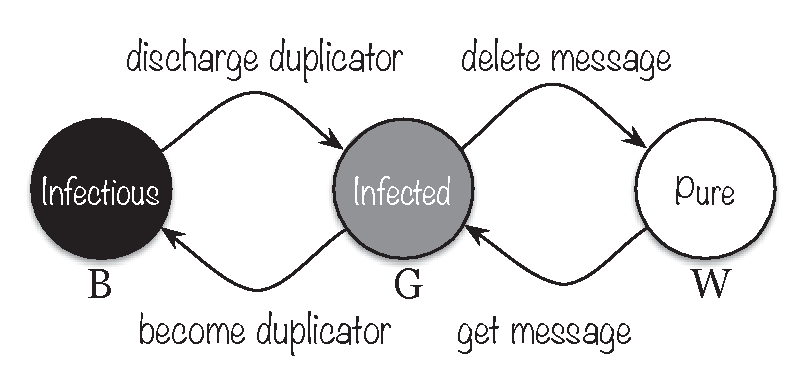
\includegraphics[width=3in]{paper-MPAR/states2}
\caption{Local-MPAR节点状态迁移图.}
\label{fig:chap3_states2}
\end{figure}

\begin{figure}[!tb]
\centering
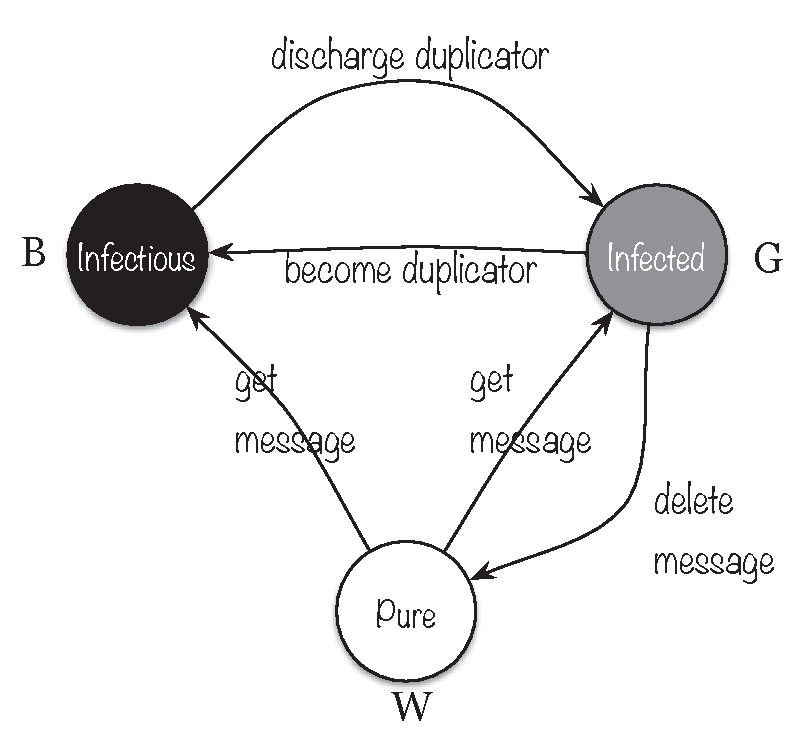
\includegraphics[width=3in]{paper-MPAR/states3}
\caption{Tabu-MPAR节点状态迁移图.}
\label{fig:chap3_states3}
\end{figure}


\begin{table*}[hbt]
\centering
  \caption{Local-MPAR中的节点状态迁移}
  \label{tab:chap3_Local-MPAR}
  \resizebox{\textwidth}{!}{
  \begin{tabular}{|c|c|c|c|c|}
  \hline

   &\multicolumn{4}{c|}{\textbf{state of $n_{b}$}}
   \\
   \hline
    \multicolumn{1}{|c|}{\multirow{9}{*}{\textbf{state of $n_{a}$}}}
   &
   & \textbf{B}
   & \textbf{G}
   & \textbf{W}
   \\
   \cline{2-5}
   & \textbf{B}
   & \multicolumn{1}{c:}{---}
   & \multicolumn{1}{c:}{B
     $\rightarrow\left\{
     \begin{array}{ll} 
      \textnormal{G} & \textnormal{if}~\textnormal{G}\rightarrow\textnormal{B happens in }n_b\\
      \textnormal{B} & \textnormal{else}
     \end{array}\right.
     $}
   & B
   \\
   \cline{2-2}\cdashline{3-5}
   & \textbf{G}
   & \multicolumn{1}{c:}{G
     $\rightarrow\left\{
     \begin{array}{ll}
      \textnormal{W} & \textnormal{if}~P_{N-\{n_a\},d}>P_{N,d} \\
      \textnormal{B} & \textnormal{if}~P_{N-\{n_a\}}\leq P_{N,d}~\textnormal{and}~E[D_a]<E[D_b] \\
      \textnormal{G} & \textnormal{else}
     \end{array}\right.
     $}
   & \multicolumn{1}{c:}{G}
   & G
   \\
   \cline{2-2}\cdashline{3-5}
   & \textbf{W}
   & \multicolumn{1}{c:}{W
     $\rightarrow\left\{
     \begin{array}{ll}
      \textnormal{G} & \textnormal{if}~P_{N\bigcup\{n_b\},d}>P_{N,d} \\
      \textnormal{W} & \textnormal{else}
     \end{array}\right.
     $}
   & \multicolumn{1}{c:}{W}
   & W
   \\
  \hline
  \end{tabular}}
\end{table*}

\begin{table*}[hbt]
\centering
  \caption{Tabu-MPAR中的节点状态迁移}
  \label{tab:chap3_Tabu-MPAR}
  \resizebox{\textwidth}{!}{
  \begin{tabular}{|c|c|c|c|c|}
  \hline

   &\multicolumn{4}{c|}{\textbf{state of $n_{b}$}}
   \\
   \hline
    \multicolumn{1}{|c|}{\multirow{9}{*}{\textbf{state of $n_{a}$}}}
   &
   & \textbf{B}
   & \textbf{G}
   & \textbf{W}
   \\
   \cline{2-5}
   & \textbf{B}
   & \multicolumn{1}{c:}{B}
   & \multicolumn{1}{c:}{
       \begin{tabular}{c}
     $B\rightarrow B|G$\\
     \textit{(depends on the tickets left in $n_a$} \\
     \textit{after allocating to $n_b$)} \\
     \end{tabular}
   }
   & 
    \begin{tabular}{c}
     $B\rightarrow B|G$\\
     \textit{(depends on the} \\
     \textit{tickets left in $n_a$} \\
     \textit{after allocating to $n_b$)} \\
     \end{tabular}
   \\
   \cline{2-2}\cdashline{3-5}
   & \textbf{G}
   & \multicolumn{1}{c:}{
   \begin{tabular}{c}
     $G\rightarrow B|G$\\
     \textit{(depends on the} \\
     \textit{tickets left in $n_a$} \\
     \textit{after allocating to $n_b$)} \\
     \end{tabular}
   }
   & \multicolumn{1}{c:}{G}
   & G
    $\rightarrow\left\{
     \begin{array}{ll}
      W & \textnormal{if}~n_a\notin N_{opt}~\textnormal{and}~n_b\in N_{opt}\\
      G & \textnormal{else}
     \end{array}\right.
    $
   \\
   \cline{2-2}\cdashline{3-5}
   & \textbf{W}
   & \multicolumn{1}{c:}{
     \begin{tabular}{c}
     $W\rightarrow B|G$\\
     \textit{(depends on the} \\
     \textit{tickets left in $n_a$} \\
     \textit{after allocating to $n_b$)} \\
     \end{tabular}
     }
   & \multicolumn{1}{c:}{W
    $\rightarrow\left\{
    \begin{array}{ll}
     \textnormal{G} & \textnormal{if}~n_a\in N_{opt}~\textnormal{and}~n_b\notin N_{opt}\\
     \textnormal{W} & \textnormal{else}
    \end{array}\right.
    $
   }
   & W
   \\
  \hline
  \end{tabular}}
\end{table*}

\begin{theorem}
\label{theorem:replication_deletion}
%The replication operation is corresponding to the transition from W to G and deletion operation to the transition from G to W.
对应\tablename~\ref{tab:chap3_Tabu-MPAR}中的状态迁移,复制操作对应于$W\rightarrow G$,删除操作对应于$G\rightarrow W$。
\end{theorem}
\begin{proof}
从三种状态的定义可知,持有消息的节点,位于状态$B$或$G$,未持有消息的节点,对应于状态$W$。由于$B$与$W$之间无直接迁移路径,状态$B$只能经过状态$G$迁移至$W$,反之亦然。从公设~\ref{post:replication}可知,复制操作对应于状态迁移$W\rightarrow B$,其中包含迁移$W\rightarrow G$。从公设~\ref{post:deletion}可知,删除操作对应于$B\rightarrow W$,即有$G\rightarrow W$。\\
证毕
\end{proof}


\subsection{Local-MPAR:基于局部搜索的路由算法}

在Local-MPAR算法中,节点可以处于三种状态中的任一状态。然而,对于每一条从源节点产生的消息而言,只允许网络中存在不超过一个传染节点。Local-MPAR的基本思想,即是动态调整集合$N$,从而最大化预测投递概率$P_{N,d}$。

算法~\ref{alg:chap3_Local-MPAR}~阐述了Local-MPAR算法的过程。在Local-MPAR中共有三种状态,在初始状态时,源节点$n_s$产生了消息$M$,于是其状态被设为传染状态。相应地,集合$N$被初始化为只包含源节点$n_s$。对于集合$N$,有如下公设。

\begin{postulation}
\label{post:N}
在Local-MPAR中, 节点集合$N$总是被传染节点维护。
\end{postulation}

算法~\ref{alg:chap3_Local-MPAR}~中整个路由过程可以被视作动态调整集合$N$的过程,如Routing Stage所示。该Stage的关键操作,即是让每一个节点完成\tablename~\ref{tab:chap3_Local-MPAR}中的状态转换。为简单起见,称表中行B列G的位置为BG。从\tablename~\ref{tab:chap3_Local-MPAR}可以看出,对于任意两个相遇节点$n_a$及$n_b$,状态迁移仅发生在$n_a$和$n_b$至少有一个处于B状态时。BB中无行为发生,其原因是在Local-MPAR中,对于某一条消息而言,不可能有两个节点同时处于B状态。


\begin{algorithm}[tbp] %算法的开始
\renewcommand{\algorithmicensure}{\textbf{Initial Stage:}}
\caption{Local-MPAR Algorithm.} %算法的标题
\label{alg:chap3_Local-MPAR} %给算法一个标签,这样方便在文中对算法的引用
\begin{algorithmic}[1] %这个1 表示每一行都显示数字
\ENSURE
\STATE $n_s$ generates message $M$
\STATE $n_s.state\leftarrow$\textbf{B}
\STATE $N\leftarrow\{n_s\}$
\end{algorithmic} %这个1 表示每一行都显示数字
\begin{algorithmic}[1] %这个1 表示每一行都显示数字
\renewcommand{\algorithmicensure}{\textbf{Routing Stage:}}
\ENSURE
\FOR{any pair of $n_a$ and $n_b$}
    \IF{$n_a$ and $n_b$ encounter}
        \STATE finish the state transition according to \tablename~\ref{tab:chap3_Local-MPAR}
        \STATE update $N$
    \ENDIF
\ENDFOR
\end{algorithmic}
\begin{algorithmic}[1]
\renewcommand{\algorithmicensure}{\textbf{End Stage:}}
\ENSURE
\STATE $M$ is delivered
\end{algorithmic}
\end{algorithm}

\begin{lemma}
\label{lemma:infectious}
%The replication or deletion of message happens only if one of the encountered two nodes is in infectious state.
消息的复制过程或删除过程,仅当相遇的两个节点中其中一个为传染节点时,才会发生。
\end{lemma}
\begin{proof}
直接由 \tablename~\ref{tab:chap3_Local-MPAR}得出。\\
证毕
\end{proof}

\begin{theorem} 
%The routing stage of Local-MPAR is a local search process in the solution space $\mathcal{S}$.
Local-MPAR的路由阶段,即在解空间$\mathcal{S}$中做局部搜索。
\end{theorem}
\begin{proof}
%From postulation~4, we know that the node set $N$ is updated only in infectious node. Lemma~1 directly shows that any happened replication or deletion operation can be informed to the infectious node immediately, so that $N$ would be updated in time. Either a replication or deletion operation just causes 1 replicas difference in the network, thus only adding or removing one element in the set $N$, which indeed transfers the correspondent solution vector to one of its neighborhoods $\mathcal{N}(N)$. We can see from \tablename~4 that N would not vary if and only if $\forall N'\in\mathcal{N}(N), P_{N',d}\leq P_{N,d}$, i.e.,  if and only if the solution reaches the local optimum.
从公设~\ref{post:N}可知,节点集合$N$只会在传染节点中被更新。引理~\ref{lemma:infectious}直接可得,任何复制或删除操作可以立即被传染节点所知,即集合$N$可被及时更新。复制操作或删除操作,其只会引起网络中一份拷贝的数量差异,因此仅仅会从集合$N$中删除或增加一个元素,其本质即是将当前解向量迁移至其某一邻居解向量。从\tablename~\ref{tab:chap3_Local-MPAR}可知,$N$当且仅当$\forall N'\in\mathcal{N}(N), P_{N',d}\leq P_{N,d}$才不会再改变;即当且仅当解向量到达局部最优时,算法停止。\\
证毕
\end{proof}

另一个需要解释的问题是,既然Local-MPAR中只存在一个传染节点,那么该节点应当如何选取?其选取的基本准则,即是基于公式~(\ref{eq:delay})中对节点移动到下一个位置的延迟时间的预测。在\tablename~\ref{tab:chap3_Local-MPAR}中GB位置,当无需将$n_a$从状态G迁移至状态W时,应当考虑是否改变$n_a$为传染节点。若$E[D_a]$的值小于$E[D_b]$,则认为$n_a$更适合担当消息复制者,因为它具有更低的移动到下一位置的期望时延,意味着更多的传输机会。反之,若将消息复制权交给$n_b$,$n_b$将发生G$\rightarrow$B迁移,对称地,$n_a$将发生B$\rightarrow$G迁移。这样网络中仍然只保持有仅一个传染节点。

\figurename~\ref{fig:chap3_example1}中例子所示的Local-MPAR路由过程,如\figurename~\ref{fig:chap3_local_rt}所示。在时间$t_1$,节点$n_2$产生目的节点为$n_4$的消息。从时间$t_2$到$t_3$,由于集合$\{n_1,n_2\}$及集合$\{n_2,n_3\}$所对应的投递率都要小于集合$\{n_2\}$,$n_2$不会向$n_1$及$n_3$复制消息。最优集合$N_{opt}=\{n_1,n_2,n_3\}$所对应的投递概率,要比$\{n_2\}$所对应的投递概率大,然而,由于Local-MPAR算法无法跳出局部最优,故$N$无法变为$N_{opt}$。

\begin{figure}
\centering
\subfigure[Time $t_1$\label{local_rt1}]
{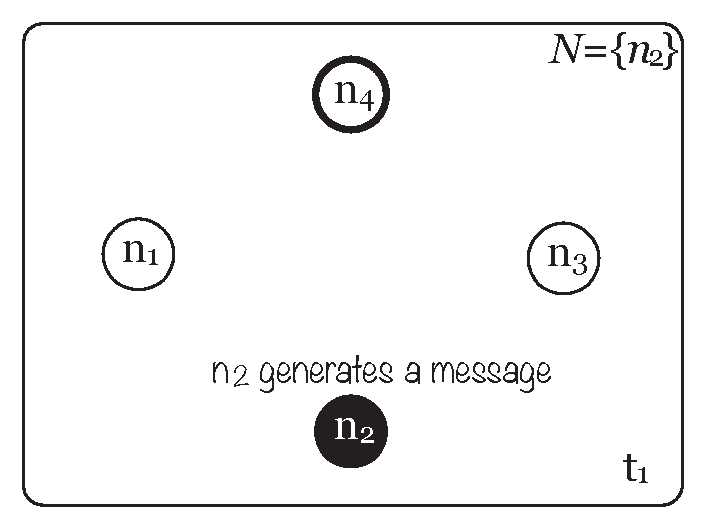
\includegraphics[width=0.45\linewidth]{paper-MPAR/local_rt1}}
\subfigure[Time $t_2$\label{local_rt2}]
{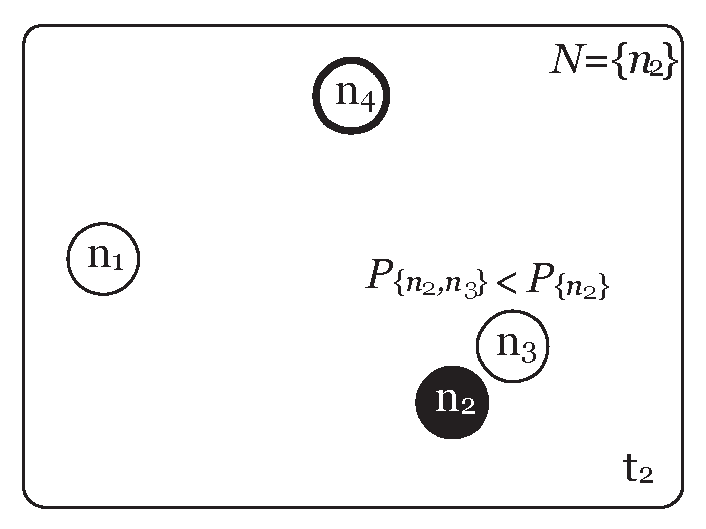
\includegraphics[width=0.45\linewidth]{paper-MPAR/local_rt2}} \\
\subfigure[Time $t_3$\label{local_rt3}]
{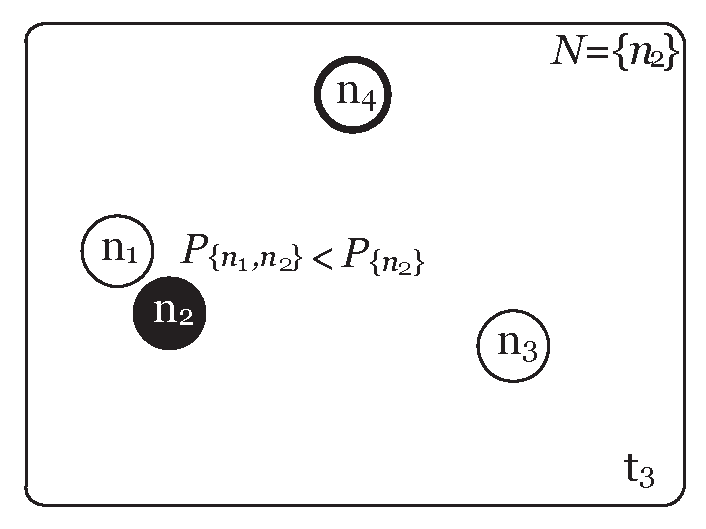
\includegraphics[width=0.45\linewidth]{paper-MPAR/local_rt3}}
\subfigure[Time $t_4$\label{local_rt4}]
{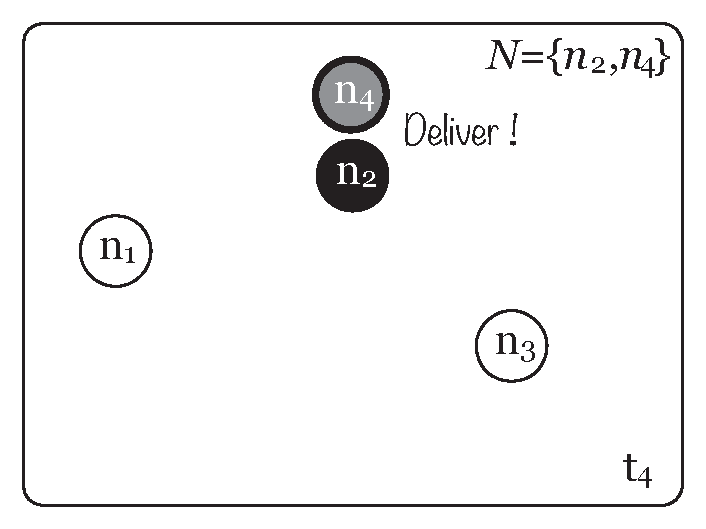
\includegraphics[width=0.45\linewidth]{paper-MPAR/local_rt4}}
\caption{Local-MPAR路由过程.}
\label{fig:chap3_local_rt}
\end{figure}

\subsection{Tabu-MPAR:基于禁忌搜索的路由算法}

在Tabu-MPAR算法中,与Local-MPAR相同,每个节点都有三个状态。如同SprayAndWait算法,允许网络中存在多于一个但有最大数目限制的传染节点。

Tabu-MPAR路由算法如算法~\ref{alg:chap3_Tabu-MPAR}所示。如同Local-MPAR, Tabu-MPAR算法亦分为三个阶段。在初始节点,当源节点$n_s$产生消息$M$时,节点$n_s$的状态被设为B,如行1--2所示。节点集合$N_{opt}$在源节点中计算,此外,对于每一条产生的消息,都对应有一个网络中该消息的最大副本数量,该值设为$|N_{opt}|$。每个节点对于每条消息,维护有一个计数变量,用以指明当前该节点持有该消息的拷贝数目。节点处于状态B,当且仅当其消息计数变量大于1\footnote{严格来讲,该节点是针对该条消息处于状态B,对于其它消息而言,该节点的状态也可能为W或者G。}.持有消息的计数变量为1的节点,处于状态G,不持有该消息的节点,皆处于状态P。

算法~\ref{alg:chap3_Tabu-MPAR}的第二阶段即是Tabu-MPAR的路由过程。与Local-MPAR相比,有两个不同点。首先,无需在路由过程中更新$N_{opt}$,因为其已在源节点$n_s$中被计算出来,并写入消息的头部。其次,当任意两个节点$n_a$及$n_b$相遇时,将在状态转换之前重新分配对应的消息计数变量。分配策略基于$E[D_a]$及$E[D_b]$的值,如行3及行4所示。具有更小$E[D]$值的节点,将被分配更多数目的消息拷贝。行5--10保证了变量$a$和$b$都是位于$1$和$L-1$之间的整数。由此可定义Tabu-MPAR的状态转换规则,如\tablename~\ref{tab:chap3_Tabu-MPAR}。除了表中对角线位置以外,其它表位置中都可能发生对应的状态迁移。事实上,当节点$n_a$发生GB位置的状态迁移时,节点$n_b$也同时发生BG位置的状态迁移,反之亦然。该规则也适用于WB,BW及WG,GW。故表\tablename~\ref{tab:chap3_Tabu-MPAR}可以看做一个$3\times 3$的对称矩阵。Tabu-MPAR路由过程如\figurename~\ref{fig:chap3_tabu_rt}所示。

\begin{algorithm}[htbp] %算法的开始
\renewcommand{\algorithmicensure}{\textbf{Initial Stage:}}
\caption{Tabu-MPAR Algorithm.} %算法的标题
\label{alg:chap3_Tabu-MPAR} %给算法一个标签,这样方便在文中对算法的引用
\begin{algorithmic}[1] %这个1 表示每一行都显示数字
\ENSURE
\STATE $n_s$ generates message $M$
\STATE $n_s.state\leftarrow$\textbf{B}
\STATE $n_s$ computes $N_{opt}$ by tabu search and saves it in $M$
\STATE $n_s.tickets\leftarrow |N_{opt}|$
\end{algorithmic} %这个1 表示每一行都显示数字
\begin{algorithmic}[1] %这个1 表示每一行都显示数字
\renewcommand{\algorithmicensure}{\textbf{Routing Stage:}}
\ENSURE
\FOR{any pair of $n_a$ and $n_b$}
    \IF{$n_a$ and $n_b$ encounter}
        \STATE $a=\frac{E[D_b]}{E[D_a]+E[D_b]}\cdot |N_{opt}|$
        \STATE $b=\frac{E[D_a]}{E[D_a]+E[D_b]}\cdot |N_{opt}|$
        \IF{$a<1$}
            \STATE $n_a.tickets=\lceil a \rceil$
            \STATE $n_b.tickets=\lfloor b \rfloor$
        \ELSE
            \STATE $n_a.tickets=\lfloor a \rfloor$
            \STATE $n_b.tickets=\lceil b \rceil$
        \ENDIF
        \STATE finish the state transition according to \tablename~\ref{tab:chap3_Tabu-MPAR}
    \ENDIF
\ENDFOR
\end{algorithmic}
\begin{algorithmic}[1]
\renewcommand{\algorithmicensure}{\textbf{End Stage:}}
\ENSURE
\STATE $M$ is delivered
\end{algorithmic}
\end{algorithm}

\begin{figure}
\centering
\subfigure[Time $t_1$\label{tabu_rt1}]
{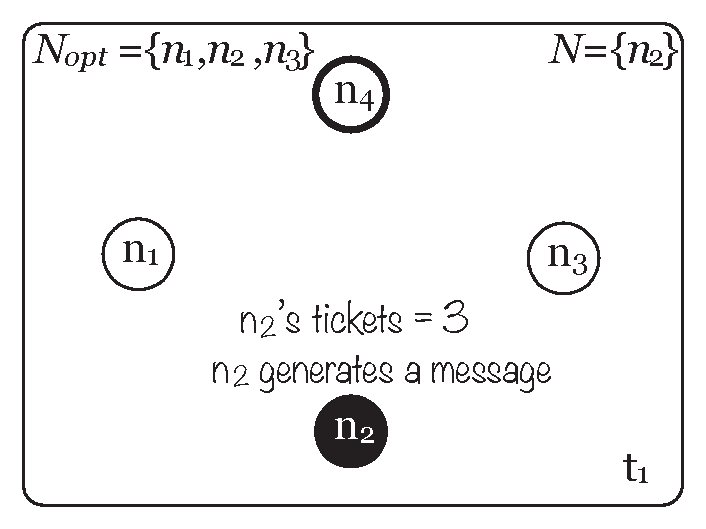
\includegraphics[width=0.45\linewidth]{paper-MPAR/tabu_rt1}}
\subfigure[Time $t_2$\label{tabu_rt2}]
{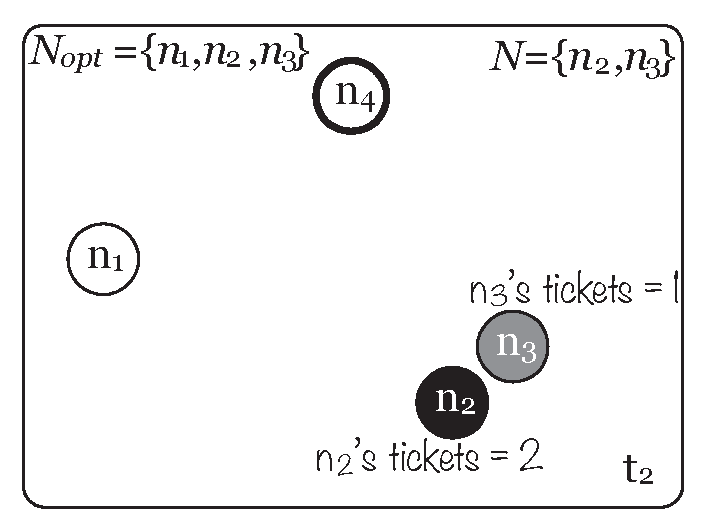
\includegraphics[width=0.45\linewidth]{paper-MPAR/tabu_rt2}} \\
\subfigure[Time $t_3$\label{tabu_rt3}]
{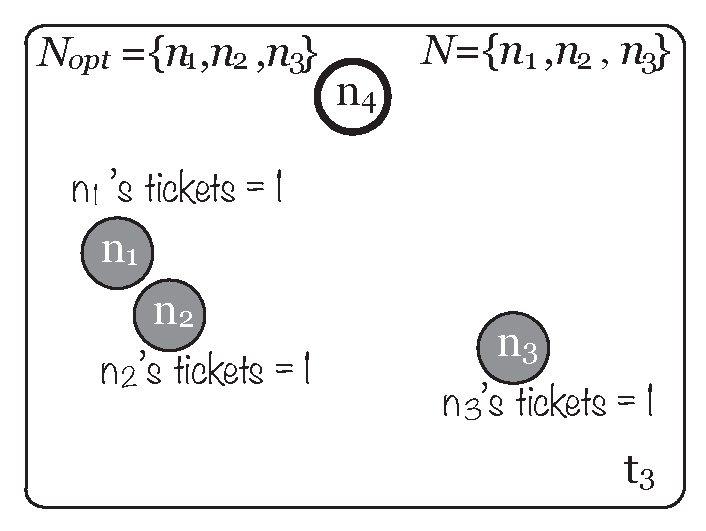
\includegraphics[width=0.45\linewidth]{paper-MPAR/tabu_rt3}}
\subfigure[Time $t_4$\label{tabu_rt4}]
{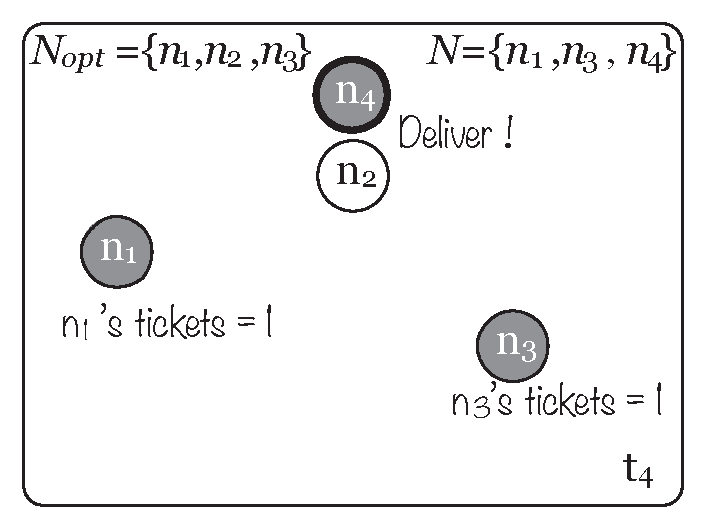
\includegraphics[width=0.45\linewidth]{paper-MPAR/tabu_rt4}}
\caption{Tabu-MPAR路由过程.}
\label{fig:chap3_tabu_rt}
\end{figure}

下面证明Tabu-MPAR的路由过程即对应$N$变为最优集合$N_{opt}$的过程。

\begin{lemma}
$N=N_{opt}$当且仅当网络中不存在传染节点时发生,即所有属于集合$N$中的节点,都处于状态G。
\label{lemma:no_infectious}
\end{lemma}
\begin{proof}
由于网络中某条消息最大副本数量为$|N_{opt}|$,若存在传染节点$n_a$,则其对应的拷贝数量至少为2,故其它节点一共所具有的拷贝数量不会超过$|N_{opt}|-2$。因此,持有该消息的所有节点的数目,至多为$|N_{opt}|-1$个,故其必要性成立。若持有该消息的节点集合为$|N_{opt}|$,则该条消息在网络中已达到其最大可能副本数量$|N_{opt}|$。在此情形下,每个节点所持有该消息的拷贝数目为1份。根据Tabu-MPAR节点状态的定义,集合$|N_{opt}|$中所有节点此时都处于被感染状态,即状态G;其它所有节点都为纯净节点,即处于状态W。此时,网络中无传染节点,故充分性成立。\\
证毕
\end{proof}



\begin{lemma}
若集合$N$变为$N_{opt}$,则不会再改变。
\label{lemma:change}
\end{lemma}
\begin{proof}
从引理~\ref{lemma:no_infectious}可知,若$N$变为$N_{opt}$,则所有$N$中的节点都处于状态G,且网络中所有的纯净节点都不在$N$中。由于网络中没有位于B状态的节点,状态迁移$B\rightarrow G$不会发生。对于状态迁移$G\rightarrow B$,若其发生,则一定伴随状态迁移$G\rightarrow W$发生;然而其只可能在处于$G$状态的节点不属于$|N_{opt}|$时发生,与题设矛盾。故集合$N$中所有节点的状态不会发生改变。\\
证毕
\end{proof}

\begin{theorem}
依\tablename~\ref{tab:chap3_Tabu-MPAR}中状态转移规则能够使集合$N$变为$N_{opt}$.
\end{theorem}
\begin{proof}
状态迁移B$\rightarrow$G不会使集合$N$发生改变。从算法~\ref{alg:chap3_Tabu-MPAR}4--10行可知,所有节点重新分配后的副本数目至少为1,即若有足够多的节点接触机会,则网络中所有处于B状态的节点最终都会变为状态G。考虑状态迁移W$\rightarrow$G及G$\rightarrow$W,其转换规则即符合$N_{opt}$。结合引理~\ref{lemma:no_infectious}及引理~\ref{lemma:change}即可证得本定理。\\
证毕
\end{proof}


\section{仿真实验}
\label{chap3:仿真实验}

在本节中,基于机会网络仿真器(Opportunistic Network Environment, ONE)\cite{Keranen2009},对MPAR算法进行仿真,并进行性能评估比较。节点移动模型采用\cite{Ekman:2008fp}提出的Working Day Movement (WDM)模型,地图设为Manhattan Blocks。WDM模型分层结合了许多子节点移动模型。此外,一些常见的移动模型相关元素,如家,办公室,夜晚活动及不同的交通工具(如电车,私家车等)也在WDM中设定,用以捕捉人类社会相关属性。办公室模型(office sub-model)产生一种围绕办公桌的星形移动轨迹,相关的办公室人员按此轨迹进行移动。家模型(home sub-model)即是使人员在某个定点固定下自身位置,不做移动。夜晚活动模型(evening activity sub-model)反映了具有朋友关系的人群在工作后的活动,其使节点在街道上服从随机走方式移动。Manhattan Community模型将节点路径限制在街道上。Manhattan Community模型包含一组呈矩阵状的小格,如\figurename~\ref{fig:chap3_manhattan}。

\begin{figure}[!t]
\centering
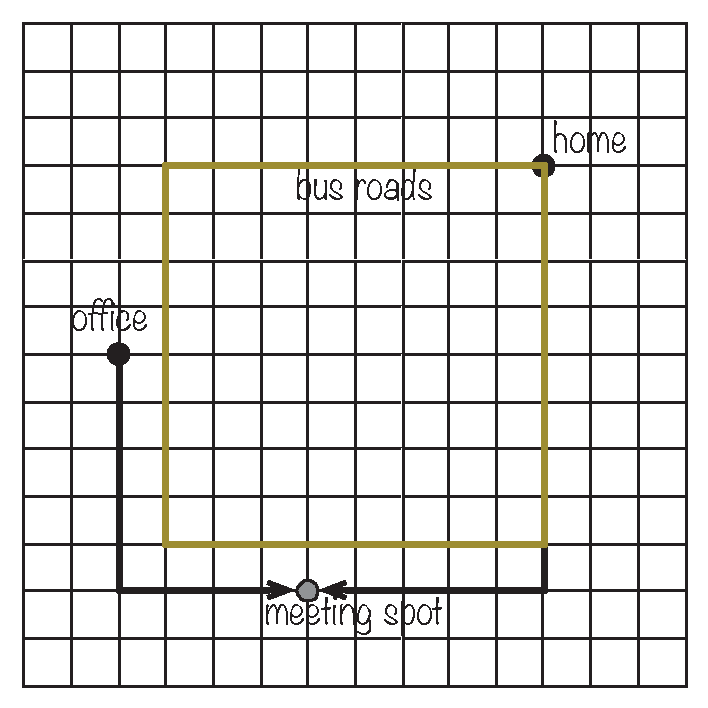
\includegraphics[width=2.7in]{paper-MPAR/Manhattan}
\caption{Working day movement模型,结合Manhattan blocks.}
\label{fig:chap3_manhattan}
\end{figure}

网络场景设定如下。行人数量分别设为200, 400, 600, 800。公交车,办公室及活动场所的数量分别设为总节点数目的2\%, 20\%, 2.5\%。在模拟器时间内,每人每天工作时间设为8小时。每人晚上参加夜晚活动的概率为0.5。此外,每个人有车的概率为0.2,若有车,则晚上参加活动将会开车,否则将乘巴士。行人的行走速度设为0.8--1.4m/s。如\figurename~\ref{fig:chap3_manhattan}所示,网络中设有三类地点,家(home),办公室(office)及聚会地点(meeting spot)。在街区中心设有一个环绕中心的公交路线,可以用于搭载行人。在每一个家,办公室及聚会地点,都设有一个throw-box,用以接管和传递消息。所有节点都以蓝牙接口通信,传输半径设为10 m,数据率设为250 KB/s。由于每一类地点(家,办公室或聚会地点)都设为地图上的一个点,仿真中确保每个节点到达这些地点后一定与throwbox发生接触。在仿真中,共产生30,000条消息,对于每条消息,其源节点和目的节点从所有行人节点中随机选择。每条消息的大小设为500 K 至 1 M 之间。仿真区域的大小根据节点数目的多少按同比例设定。对于整个仿真过程,其仿真器时间设为12天。

本节将MPAR算法与两个经典算法相比较:Delegation Forwarding (DF) \cite{Erramilli2008}与Simbet \cite{Daly2007}。采用四项评估指标:投递率(delivery ratio),平均时延(average latency),网络开销(overhead ratio)及平均每跳数(average hop count)。



\subsection{自变量:消息生存时间}

节点缓存大小固定在200M。消息的生存时间在10小时到30小时变化,仿真结果如\figurename~\ref{fig:chap3_delivery_ttl},\figurename~\ref{fig:chap3_latency_ttl},\figurename~\ref{fig:chap3_overhead_ttl},\figurename~\ref{fig:chap3_hop_ttl}。

仿真结果表明,两种MPAR算法,Local-MPAR及Tabu-MPAR,其性能表现都要优于DF及SimBet。与DF算法相比,Tabu-MPAR和Local-MPAR分别可以增加约71.1\%及37.8\%的消息投递率,且能降低约83.8\%及57.8\%的平均时延。与SimBet算法相比,Tabu-MPAR和Local-MPAR分别可以增加95.2\%和55.3\%的投递率,且能降低大概79.2\%及60.1\%的平均时延。从\figurename~\ref{fig:chap3_overhead_ttl}可以看出,Tabu-MPAR和Local-MPAR具有比DF及SimBet更低的网络开销。对于三中社会属性相关的路由算法,Tabu-MPAR, Local-MPAR及SimBet而言,网络开销要比DF低很多,特别是在消息生存时间设为比较长时。当网络中节点数目更小时,这种提升就越明显。由于MPAR路由算法限制了消息的最大副本数量,且利用throwbox辅助投递消息,中继传输操作非常少。此外,随着节点数目的增加,对于每个节点而言,其开销也会相应减小,导致整个网络的开销减小。\figurename~\ref{fig:chap3_hop_ttl}显示了消息平均跳数的性能表现。可以看出,两种MPAR算法具有比DF和SimBet更低的平均跳数。当节点数目增加时,平均跳数也增加;其原因是仿真区域按同比例增加后,需要节点间更多的合作,用以投递消息。



\subsection{自变量:节点缓存}

消息生存时间固定为仿真器中的16小时。节点缓存大小在50 MB 到 300 MB 之间变换。仿真结果如\figurename~\ref{fig:chap3_delivery_buffer},\figurename~\ref{fig:chap3_latency_buffer},\figurename~\ref{fig:chap3_overhead_buffer},\figurename~\ref{fig:chap3_hop_buffer}。

仿真结果表明,两种MPAR算法,Local-MPAR及Tabu-MPAR,其性能表现皆优于DF及SimBet。与DF算法相比,Tabu-MPAR和Local-MPAR分别可以增加约83.8\%及40.3\%的消息投递率,且能降低约83.8\%及57.8\%的平均时延。与SimBet算法相比,Tabu-MPAR和Local-MPAR分别可以增加3倍和2.5的投递率,且能降低大概80\%及60\%的平均时延。从\figurename~\ref{fig:chap3_overhead_buffer}可以看出,Tabu-MPAR和Local-MPAR具有几乎相同的网络开销;当缓存大小设为120 MB 时,MPAR算法的网络开销比SimBet略低一点,比DF低很多。当网络中节点数目更小时,性能提升越明显,如\figurename~\ref{fig:chap3_overhead_buffer}所示。与消息生存时间作为变量时相同,从\figurename~\ref{fig:chap3_hop_buffer}可以看出,两种MPAR算法具有比DF和SimBet更低的消息平均跳数,且当节点数目增加时,平均跳数也随之增加。


\begin{figure}[htbp]
\centering
\subfigure[Number of nodes: $|\overline{N}|=200$\label{200_delivery_ttl}]
{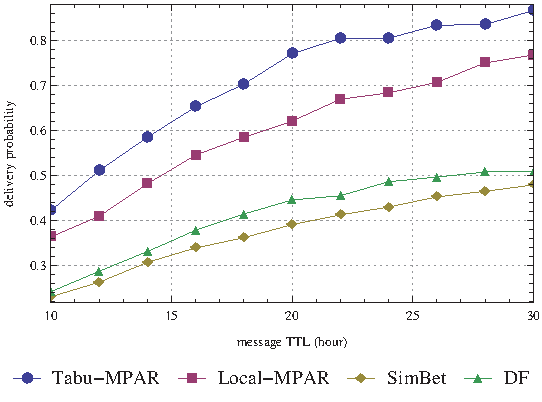
\includegraphics[width=0.37\textwidth]{paper-MPAR/200_delivery_ttl}}\quad\quad
\subfigure[Number of nodes: $|\overline{N}|=400$\label{400_delivery_ttl}]
{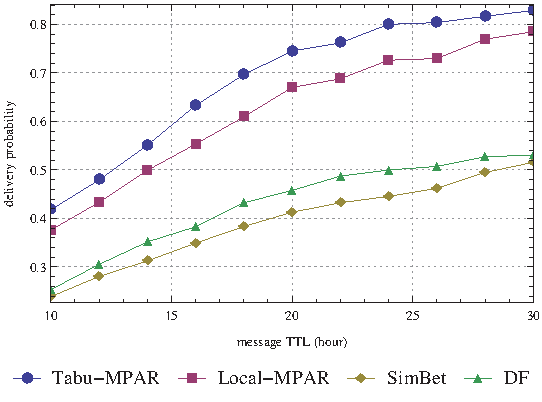
\includegraphics[width=0.37\textwidth]{paper-MPAR/400_delivery_ttl}} \\
\subfigure[Number of nodes: $|\overline{N}|=600$\label{600_delivery_ttl}]
{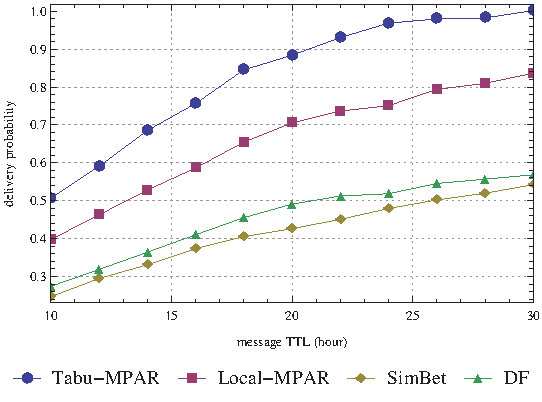
\includegraphics[width=0.37\textwidth]{paper-MPAR/600_delivery_ttl}}\quad\quad
\subfigure[Number of nodes: $|\overline{N}|=800$\label{800_delivery_ttl}]
{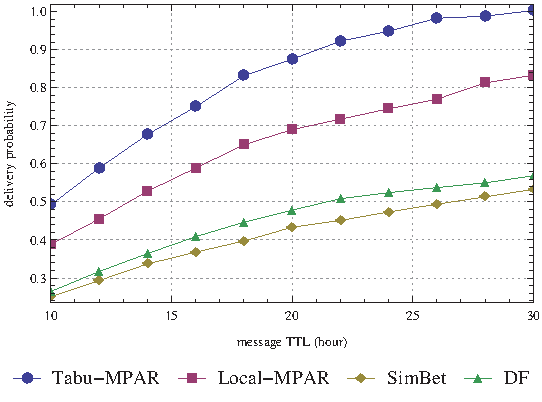
\includegraphics[width=0.37\textwidth]{paper-MPAR/800_delivery_ttl}}
\caption{消息投递率 vs. 消息生存时间}
\label{fig:chap3_delivery_ttl}
\end{figure}

\begin{figure}[htbp]
\centering
\subfigure[Number of nodes: $|\overline{N}|=200$\label{200_avgLatency_ttl}]
{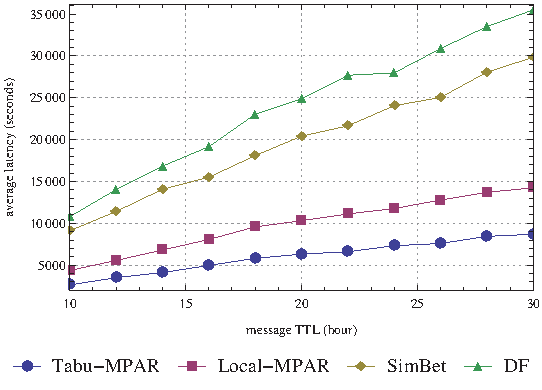
\includegraphics[width=0.37\textwidth]{paper-MPAR/200_avgLatency_ttl}}\quad\quad
\subfigure[Number of nodes: $|\overline{N}|=400$\label{400_avgLatency_ttl}]
{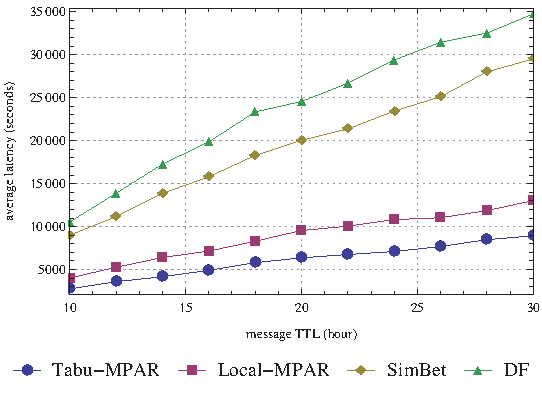
\includegraphics[width=0.37\textwidth]{paper-MPAR/400_avgLatency_ttl}} \\
\subfigure[Number of nodes: $|\overline{N}|=600$\label{600_avgLatency_ttl}]
{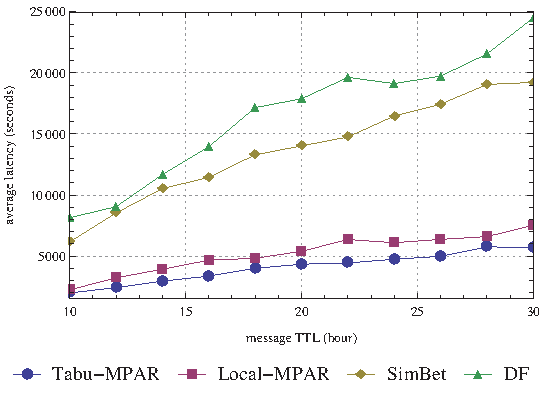
\includegraphics[width=0.37\textwidth]{paper-MPAR/600_avgLatency_ttl}}\quad\quad
\subfigure[Number of nodes: $|\overline{N}|=800$\label{800_avgLatency_ttl}]
{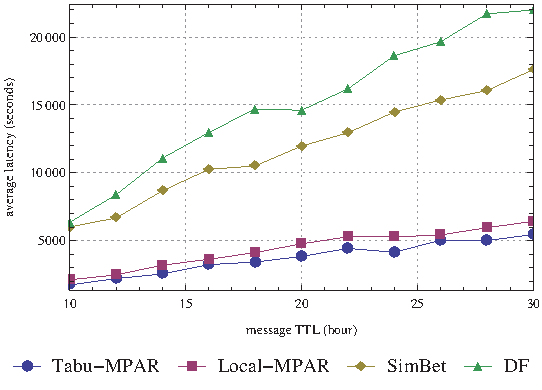
\includegraphics[width=0.37\textwidth]{paper-MPAR/800_avgLatency_ttl}}
\caption{端到端平均时延 latency vs. 消息生存时间}
\label{fig:chap3_latency_ttl}
\end{figure}

\begin{figure}[htbp]
\centering
\subfigure[Number of nodes: $|\overline{N}|=200$\label{200_overhead_ttl}]
{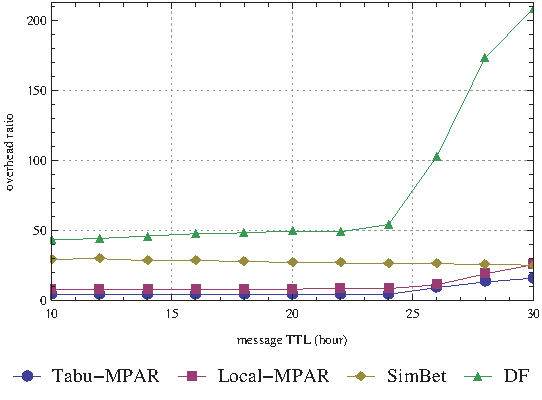
\includegraphics[width=0.37\textwidth]{paper-MPAR/200_overhead_ttl}}\quad\quad
\subfigure[Number of nodes: $|\overline{N}|=400$\label{400_overhead_ttl}]
{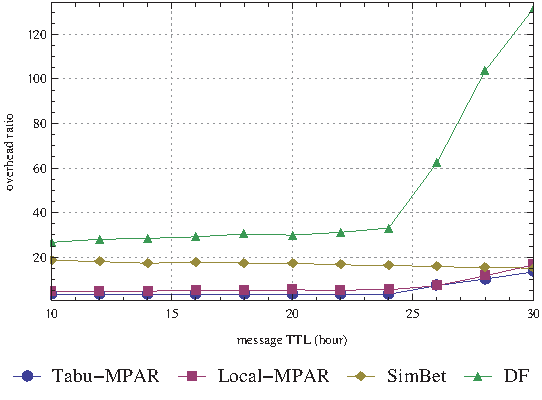
\includegraphics[width=0.37\textwidth]{paper-MPAR/400_overhead_ttl}} \\
\subfigure[Number of nodes: $|\overline{N}|=600$\label{600_overhead_ttl}]
{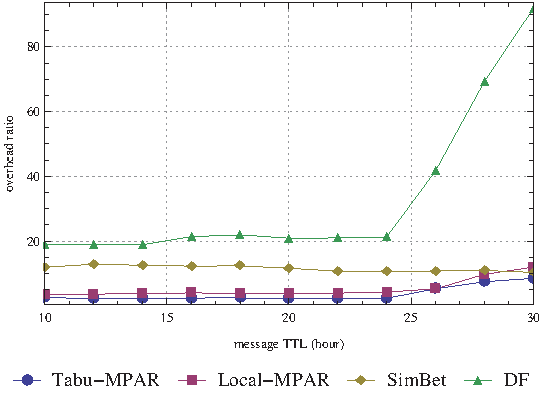
\includegraphics[width=0.37\textwidth]{paper-MPAR/600_overhead_ttl}}\quad\quad
\subfigure[Number of nodes: $|\overline{N}|=800$\label{800_overhead_ttl}]
{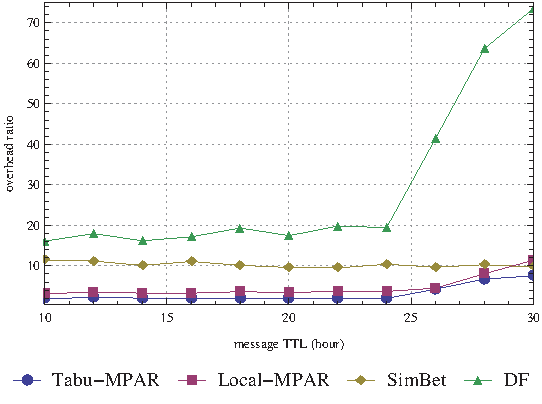
\includegraphics[width=0.37\textwidth]{paper-MPAR/800_overhead_ttl}}
\caption{网络开销 vs. 消息生存时间}
\label{fig:chap3_overhead_ttl}
\end{figure}

\begin{figure}[htbp]
\centering
\subfigure[Number of nodes: $|\overline{N}|=200$\label{200_avgHop_ttl}]
{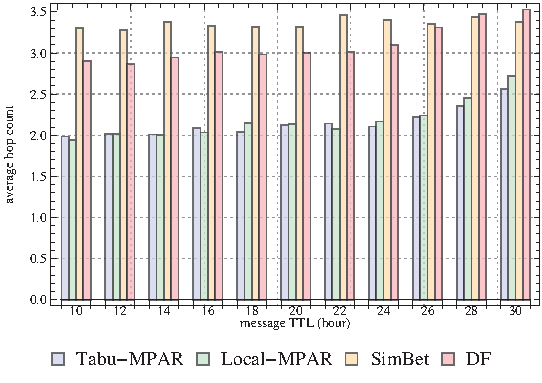
\includegraphics[width=0.37\textwidth]{paper-MPAR/200_avgHop_ttl}}\quad\quad
\subfigure[Number of nodes: $|\overline{N}|=400$\label{400_avgHop_ttl}]
{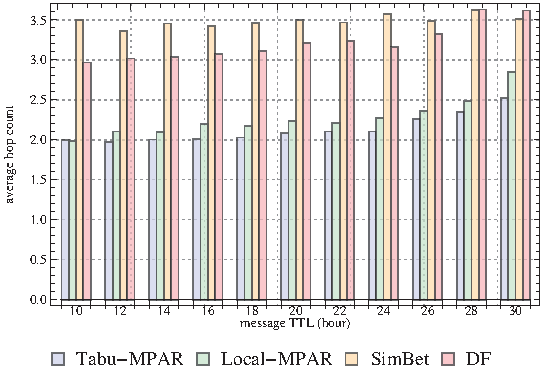
\includegraphics[width=0.37\textwidth]{paper-MPAR/400_avgHop_ttl}} \\
\subfigure[Number of nodes: $|\overline{N}|=600$\label{600_avgHop_ttl}]
{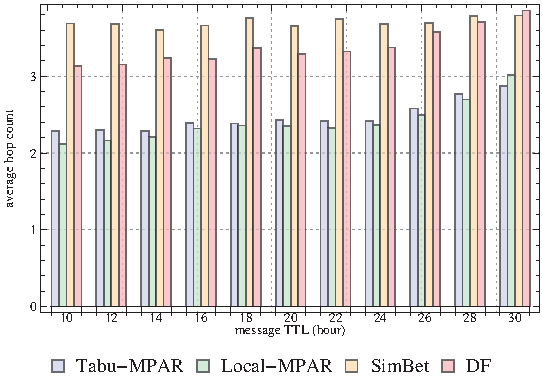
\includegraphics[width=0.37\textwidth]{paper-MPAR/600_avgHop_ttl}}\quad\quad
\subfigure[Number of nodes: $|\overline{N}|=800$\label{800_avgHop_ttl}]
{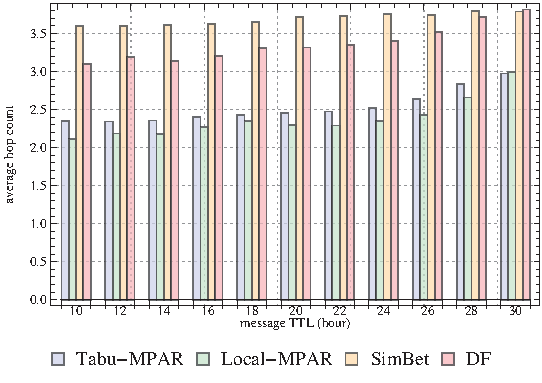
\includegraphics[width=0.37\textwidth]{paper-MPAR/800_avgHop_ttl}}
\caption{平均跳数 vs. 消息生存时间}
\label{fig:chap3_hop_ttl}
\end{figure}

\begin{figure}[htbp]
\centering
\subfigure[Number of nodes: $|\overline{N}|=200$\label{200_delivery_buffer}]
{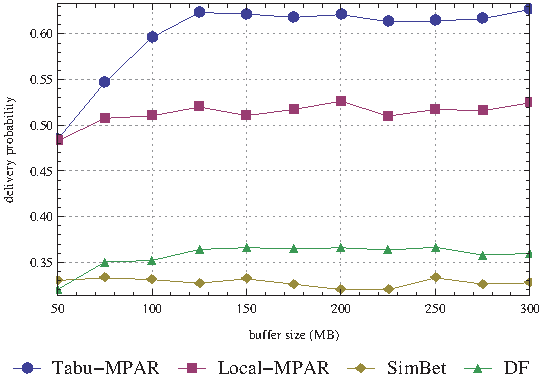
\includegraphics[width=0.37\textwidth]{paper-MPAR/200_delivery_buffer}}\quad\quad
\subfigure[Number of nodes: $|\overline{N}|=400$\label{400_delivery_buffer}]
{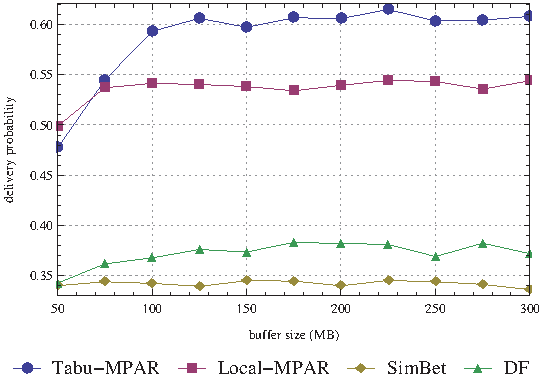
\includegraphics[width=0.37\textwidth]{paper-MPAR/400_delivery_buffer}} \\
\subfigure[Number of nodes: $|\overline{N}|=600$\label{600_delivery_buffer}]
{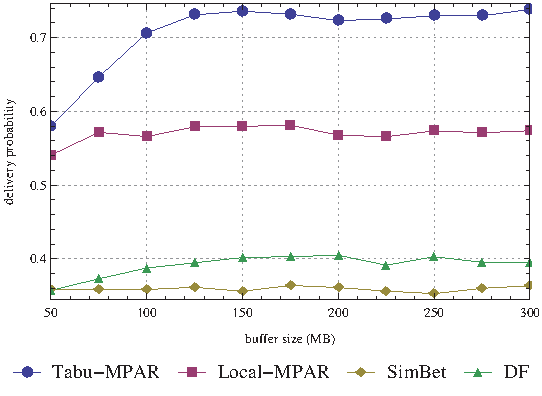
\includegraphics[width=0.37\textwidth]{paper-MPAR/600_delivery_buffer}}\quad\quad
\subfigure[Number of nodes: $|\overline{N}|=800$\label{800_delivery_buffer}]
{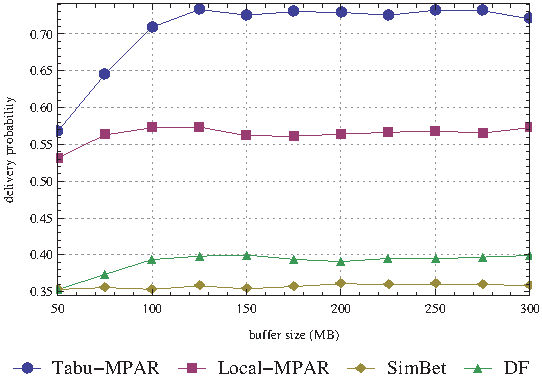
\includegraphics[width=0.37\textwidth]{paper-MPAR/800_delivery_buffer}}
\caption{消息投递率 vs. 节点缓存}
\label{fig:chap3_delivery_buffer}
\end{figure}

\begin{figure}[htbp]
\centering
\subfigure[Number of nodes: $|\overline{N}|=200$\label{200_avgLatency_buffer}]
{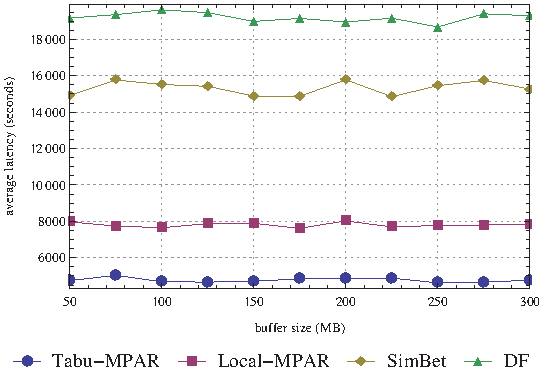
\includegraphics[width=0.37\textwidth]{paper-MPAR/200_avgLatency_buffer}}\quad\quad
\subfigure[Number of nodes: $|\overline{N}|=400$\label{400_avgLatency_buffer}]
{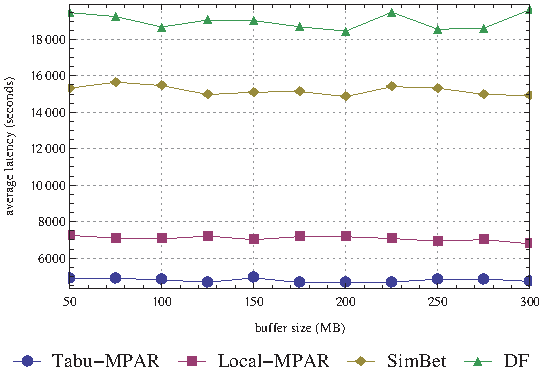
\includegraphics[width=0.37\textwidth]{paper-MPAR/400_avgLatency_buffer}} \\
\subfigure[Number of nodes: $|\overline{N}|=600$\label{600_avgLatency_buffer}]
{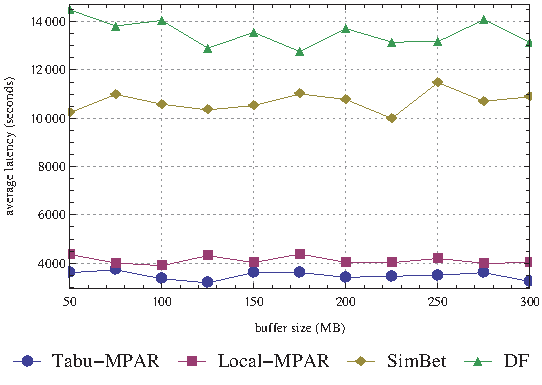
\includegraphics[width=0.37\textwidth]{paper-MPAR/600_avgLatency_buffer}}\quad\quad
\subfigure[Number of nodes: $|\overline{N}|=800$\label{800_avgLatency_buffer}]
{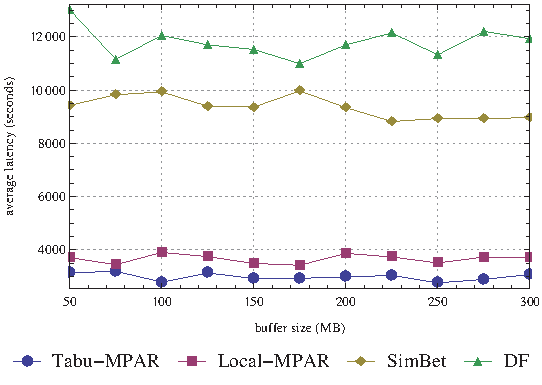
\includegraphics[width=0.37\textwidth]{paper-MPAR/800_avgLatency_buffer}}
\caption{端到端平均时延 vs. 节点缓存}
\label{fig:chap3_latency_buffer}
\end{figure}

\begin{figure}[htbp]
\centering
\subfigure[Number of nodes: $|\overline{N}|=200$\label{200_overhead_buffer}]
{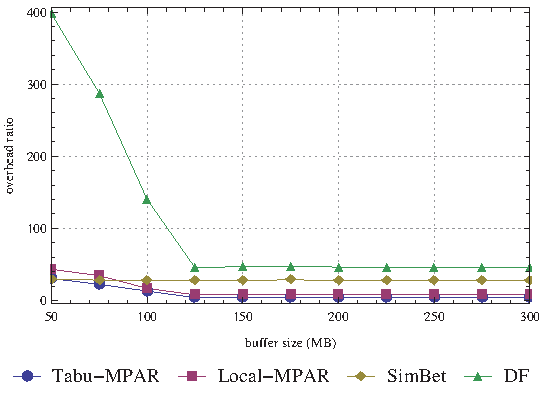
\includegraphics[width=0.37\textwidth]{paper-MPAR/200_overhead_buffer}}\quad\quad
\subfigure[Number of nodes: $|\overline{N}|=400$\label{400_overhead_buffer}]
{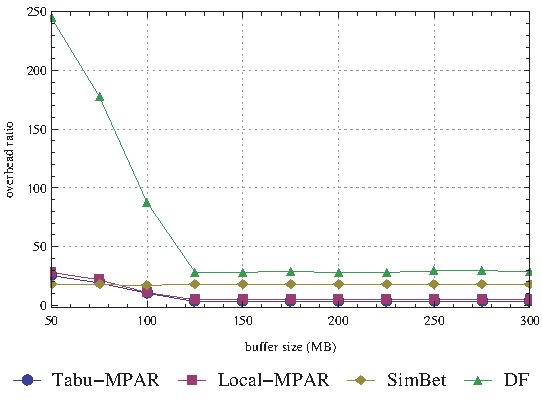
\includegraphics[width=0.37\textwidth]{paper-MPAR/400_overhead_buffer}} \\
\subfigure[Number of nodes: $|\overline{N}|=600$\label{600_overhead_buffer}]
{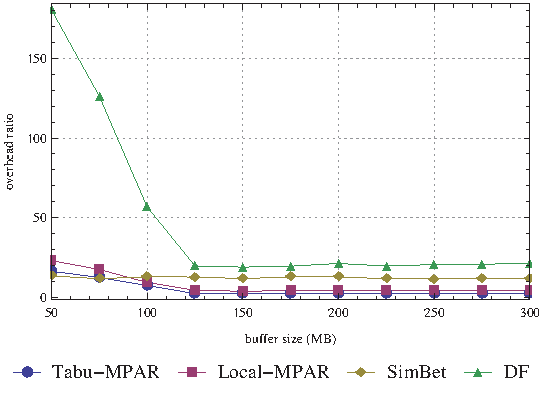
\includegraphics[width=0.37\textwidth]{paper-MPAR/600_overhead_buffer}}\quad\quad
\subfigure[Number of nodes: $|\overline{N}|=800$\label{800_overhead_buffer}]
{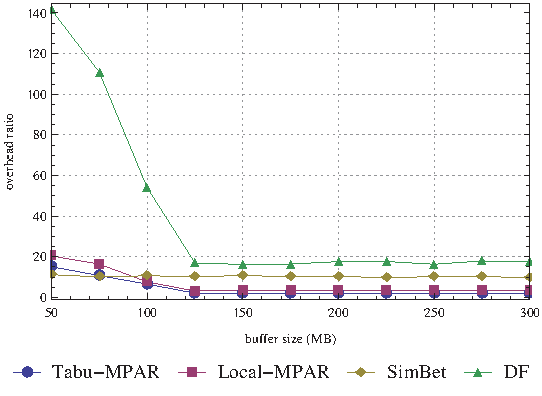
\includegraphics[width=0.37\textwidth]{paper-MPAR/800_overhead_buffer}}
\caption{网络开销 vs. 节点缓存}
\label{fig:chap3_overhead_buffer}
\end{figure}

\begin{figure}[htbp]
\centering
\subfigure[Number of nodes: $|\overline{N}|=200$\label{200_avgHop_buffer}]
{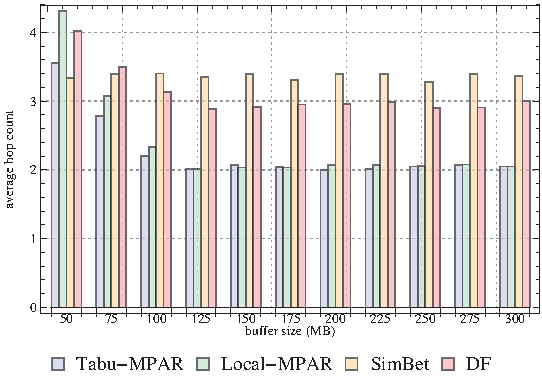
\includegraphics[width=0.37\textwidth]{paper-MPAR/200_avgHop_buffer}}\quad\quad
\subfigure[Number of nodes: $|\overline{N}|=400$\label{400_avgHop_buffer}]
{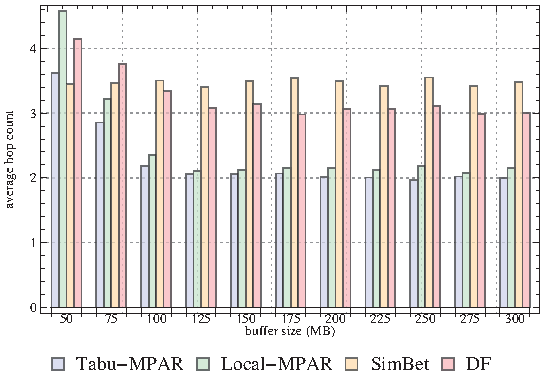
\includegraphics[width=0.37\textwidth]{paper-MPAR/400_avgHop_buffer}} \\
\subfigure[Number of nodes: $|\overline{N}|=600$\label{600_avgHop_buffer}]
{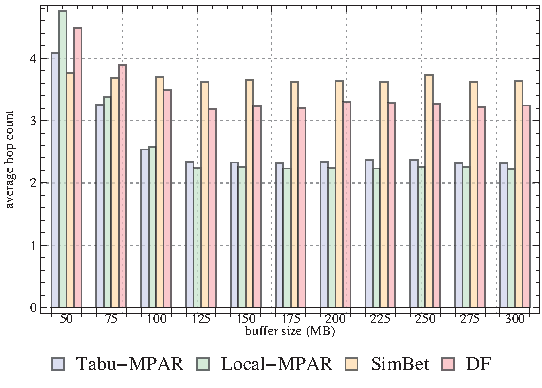
\includegraphics[width=0.37\textwidth]{paper-MPAR/600_avgHop_buffer}}\quad\quad
\subfigure[Number of nodes: $|\overline{N}|=800$\label{800_avgHop_buffer}]
{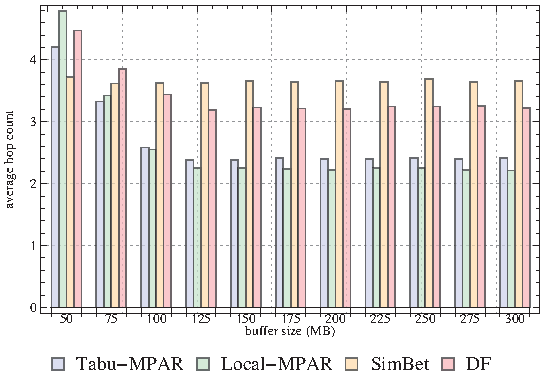
\includegraphics[width=0.37\textwidth]{paper-MPAR/800_avgHop_buffer}}
\caption{平均跳数 vs. 节点缓存}
\label{fig:chap3_hop_buffer}
\end{figure}


\section{本章总结}
\label{chap3:本章总结}
在本章中,建立了周期相关的移动记录模型,并从移动记录中提取出节点(群组)移动模式。对于成组的节点,其被看做一个整体,并评估整体的预测投递率。本章研究了两个相关路由的关键属性,并将路由问题建模为组合最优化问题,且证明了该问题的$\mathcal{NP}$难解性。为求解该路由问题,基于局部搜索及禁忌搜索,分别提出了两种路由算法Local-MPAR及Tabu-MPAR。此外,本章证明了Tabu-MPAR过程可以使得持有消息的节点集合最终达到预测投递概率最优的集合。仿真实验表明,两种MPAR算法,在机会网络中的综合移动模型WDM上优于DF算法及SimBet算法。

~\\
~\\
~\\
~\\
~\\
~\\
~\\
~\\
~\\
~\\



\chapter{基于消息传输收益的最优队列调度算法}

本章尝试改进经典的基于概率预测的路由算法PRoPHET \cite{AndersLindgren2004}。定义了“传输收益”概念,基于此,提出了传输收益最优化,吞吐量相关的概率路由问题(Optimal Throughput-Aware Probabilistic Routing)。该问题被建模为最优决策问题,并在本章中采用动态规划方法解决。在该模型下,提出了一种数据项选择机制,其具有如下特点:
\begin{enumerate}
\item 每一对节点所对应的潜在连接,其平均数据吞吐量可能比缓存中的消息大小要小。
\item 每次传输的能量消耗不可忽略,换言之,消息传输不成功会带来无收益的能量损耗。
\end{enumerate}

例如,针对某条消息的一次传输操作而言,若当前连接所允许的总数据量比消息的大小小很多,则该次传输终止时,消息并未被成功传输。针对该问题的一个解决办法,即是总是传输不超过该连接平均吞吐量大小的消息,从而避免浪费传输机会。退一步而言,即使连接的吞吐量完全足够传输每一条消息,传输不同消息所带来的收益也并不相同(比如投递率收益,及投递时延收益等),然而传输的机会是有限的,故针对每一次传输机会而言,传输不同的消息对路由的整体性能表现具有较大的影响。从这个角度而言,在机会网络中,为了提高路由性能表现,应当设计有效的数据项选择机制。

本章组织如下:\ref{chap4:系统模型}节中介绍了系统模型及路由模型;\ref{chap4:问题形式化}节中形式化定义了关键问题;\ref{chap4:基于数据项选择的改进路由}节中利用设计的数据项选择机制对PRoPHET进行改进;\ref{chap4:仿真实验}节为仿真实验;\ref{chap4:本章小结}节概括了本章内容。

\section{系统模型}
\label{chap4:系统模型}

\begin{table*}
\centering
  \caption{数学符号}
    \label{tab:chap4_notations}
  \begin{tabular}{p{0.23\linewidth}<{\centering}p{0.7\linewidth}<{\centering}}
  \hline
    \textbf{Notation} & \textbf{Meaning}  \\
    \hline
   $\mathcal{N}$ & 网络节点集合 \\
   $n_i$ &  第 $i$ 号节点  \\
   $m_i$ &  第 $i$ 号消息 \\
   $TTL(i)$ & 消息 $m_i$ 的生存时间\\
   $S(i)$   & 消息 $m_i$ 的大小\\
    $\zeta(i)$ & 消息 $m_i$ 的传输收益\\
    $B_{(a,b)}$ & 节点 $n_a$ 与 $n_b$ 之间的带宽\\
   $t_{s_{(a,b)}}/t_{e_{(a,b)}}$   &  节点 $n_a$ and $n_b$ 最近一次连接的开始/结束时间\\
   $\tau_{a,b}$ & 节点 $n_a$ 与 $n_b$ 预测接触时间\\
  $P_{(a,b)}$ & $n_a$'s 节点 $n_a$ 与 $n_b$ 的预测接触概率 \\
  $ETH_{(a,b)}$ & 节点 $n_a$ 与 $n_b$ 连接的预测吞吐量\\
$P^{\{a,b\}}$ & 节点 $n_a$ 与 $n_b$ 的共同投递率\\
   \hline
  \end{tabular}
\end{table*}

数学符号如\tablename~\ref{tab:chap4_notations}所示。本模型的时间线设为离散时间,时间轴被划分为多个小的时间槽,每个时间槽的长度定义为一个单位时间。整个节点集合用符号$\mathcal{N}=\{n_i|n_i\in\mathcal{N},1\leq i<|\mathcal{N}|\}$。对于任意一条消息$m_k$,其消息生存时间表示为$TTL(k)$。当消息$m_k$被某节点产生时,$TTL(k)$的值即被指定。若某条消息的$TTL$到期,则消息会被当前节点丢弃。消息$m_k$的大小用符号$S(k)$表示。模型假设任一节点$n_i$知道其自身接口的带宽$B(i)$。该假设的合理性建立在网络中的每个节点往往在通信时都采用统一标准的某种接口,如蓝牙,wifi等。退一步讲,即使接口状态不稳定,也可以利用滑动窗口法对其平均值进行预测。对于任意一对相遇节点$n_i$及$n_j$,令节点$n_i$记录两个值$t_{s_{(i,j)}}$及$t_{e_{(i,j)}}$,分别用于记录两节点间最近一次连接的开始时间及结束时间。于是$t_{e_{(i,j)}}-t_{s_{(i,j)}}$即代表该次连接的持续时间;为简单起见,符号$t_{s_{(i,j)}}$及$t_{e_{(i,j)}}$在无歧义的上下文中,简记为$t_s$和$t_e$。

PRoPHET路由算法\cite{AndersLindgren2004}记录了节点的相遇历史,用于预测节点间的相遇概率,并且考虑到了相遇概率具有传递性的特点。在PRoPHET中,$P_{(a,b)}$即用于衡量节点$n_a$及$n_b$之间投递概率的效用函数,存于节点$n_a$内。$P_{(a,b)}$的计算及更新方法如下式所示。

\begin{equation}
P_{(a,b)}=P_{(a,b)_{old}}+(1-P_{(a,b)_{old}})\times P_{init}
\label{eq:prophet1}
\end{equation}
\begin{equation}
P_{(a,b)}=P_{(a,b)_{old}}\times\gamma^{k}
\label{eq:prophet2}
\end{equation}
\begin{equation}
P_{(a,c)}=P_{(a,c)_{old}}+(1-P_{(a,c)_{old}})\\
\times P_{(a,b)}\times P_{(b,c)}\times \beta
\label{eq:prophet3}
\end{equation}

其中,$P_{init}$, $\beta$及$\gamma$是位于$[0,1]$范围内的常数。每个节点维护一个$1\times|\mathcal{N}|$的向量,该向量中第$i$个元素记录了节点$n_a$对节点$n_i$的投递率。

\section{问题形式化}
\label{chap4:问题形式化}

本节给出问题的形式化定义。

\subsection{问题目标}
问题目标即是最大化每条消息的投递概率。在机会网络中,每个节点以“存储-携带-转发”的方式对消息进行路由。在机会路由中,一种策略是总是让节点选择对目的节点投递率高的消息进行投递。吞吐量与节点间的接触时间及通信接口带宽具有很强的相关性,因此对消息是否能投递成功具有较大的影响。然而在该种方法中,节点之间连接的吞吐量因素并未考虑进去。由于节点的带宽,接触时间及接触机会非常有限,缓存消息队列的调度策略对路由性能表现具有很大的影响。假设节点$n_a$持有三条消息$m_i$, $m_j$及$m_k$,其目的节点都为$n_b$,大小分别为150 K, 200 K 与100 K。然而当前连接最多只能传输120 K 的数据量。在此情况下,由于连接吞吐量的限制,消息$m_i$和$m_j$都无法被成功传递。一种做法是让$n_a$按消息大小从小到大传递,然而这种方法虽然能保证部分消息成功传输,但并未设定任何优化目标,由此可能使得某些虽然大小稍大,但也能成功传递,且对投递率具有较大改进的消息无法充分利用该次机会传输。为解决此问题,需要对消息的调度设定一个可行的评估指标。在本章中,主要集中研究如何有效的数据项选择机制提高消息的投递率。下面将给出最优化消息传输投递率收益的分析过程。

若消息被节点$n_a$转发给$n_b$,则该消息宣告传输失败,仅当$n_a$及$n_b$都未成功传输该消息,其投递率可以用公式(\ref{eq:probability})计算。

\begin{equation}
P^{\{a,b\}}=1-(1-P_{(a,d_i)})(1-P_{(b,d_i)})
\label{eq:probability}
\end{equation}

于是对于传输收益有如下定义。

\begin{definition}传输收益.\\
传输收益函数$\zeta(i)$用于衡量消息$m_i$在本次传输过程中能够改善的投递率, 有
\begin{equation}
\zeta(i)=P^{\{a,b\}}-P^{\{a\}}\\
=1-(1-P_{(a,d_i)})(1-P_{(b,d_i)})-P_{(a,d_i)}
\label{eq:improve}
\end{equation}
\end{definition}

函数$\zeta(i)$的值代表将消息$m_i$从节点$n_a$传输给节点$n_b$所带来的投递率收益。从这点出发,可以如下定义“吞吐量相关最优机会路由”概念。

\begin{definition} 吞吐量相关最优机会路由. \\
最优机会路由总是尝试最大化消息投递概率,且考虑带宽及接触时间两个因素。节点$n_i$将依照$\zeta$函数值选择消息传输给节点$n_j$,利用预测的吞吐量最大化$\zeta$值总和。
\label{def:throughput-routing}
\end{definition}

例如,在\tablename~\ref{tab:chap4_zeta} 所示例子中,节点$n_a$缓存中总共有5条消息,记为$m_1$, $m_2$, $m_3$, $m_4$, $m_5$。消息$m_i$的目的节点记为$d_i$。对于其中任意一条消息$m_i~(1\leq i\leq 5)$,有$P_{(b,d_i)}>P_{(a,d_i)}$。在这种情形下,当节点$n_a$与$n_b$相遇时,所有这5条消息都应由$n_a$转发给$n_b$。由公式~(\ref{eq:improve})可以得到每条消息对应的$\zeta$值。在下一小节中,将给出吞吐量的预测方法,然后给出问题的形式化定义。

\begin{table}
\centering
  \caption{节点$n_a$缓存中的5条消息}
  \label{tab:chap4_zeta}
  \begin{tabular}{cccccc}
  \hline
    data item  & $m_1$ & $m_2$ & $m_3$ & $m_4$ & $m_5$ \\
    \hline
    $P_{(a,d_i)}$ & 0 & 0.2 & 0.1 & 0.12 & 0.2 \\
    $P_{(b,d_i)}$ & 0.1  & 0.75  & 0.2 & 0.25 & 0.35  \\
    value of $\zeta$ & 0.1 & 0.6 & 0.18 & 0.22 & 0.28 \\
    message size & 1K  & 2K  & 5K   & 6K   & 7K   \\
    \hline
  \end{tabular}
\end{table}

\subsection{吞吐量预测}
\label{sec:吞吐量预测}

\begin{definition}连接吞吐量. \\
给定任意两个节点的接触时间 $t$,以及带宽 $B$ (KB/unit) , 该次连接的吞吐量,记为 $TH$ ,有
\[
TH=B\cdot t
\]
\label{def:throughput}
\end{definition}

在此假设带宽$B$为已知,要预测吞吐量,则只需预测出连接的持续时间$t$。采用公式~(\ref{eq:estimate})~预测下一次$n_a$与$n_b$之间连接的持续时间。
\begin{equation}
\tau_{(a,b)_{new}}=(1-\alpha)\tau_{(a,b)_{old}}+\alpha(t_e-t_s)
\label{eq:estimate}
\end{equation}
其中$\alpha\in[0,1]$是常数参数,$t_e-t_s$是节点$n_a$与$n_b$之间最近一次连接的持续时间,该部分加权为$\alpha$。当$\alpha$值设的较大时,公式~(\ref{eq:estimate})后半部分的影响较大,反之亦然。

当节点$n_a$一段时间内没有再与节点$n_b$接触时,则用公式~(\ref{eq:estimate2})更新$\tau_{(a,b)}$。
\begin{equation}
\tau_{(a,b)_{new}}=\tau_{(a,b)_{old}}\gamma^{k}
\label{eq:estimate2}
\end{equation}
其中$\gamma\in[0,1)$是衰减常数,如公式~(\ref{eq:prophet2})一样;$k$是离上一次更新公式流逝的单位时间数目(即经过的时间槽数目)。

在每个时间槽内,对于任意一对节点$n_a$和$n_b$,在每一个时间槽,节点都会检查$n_a$及$n_b$的连接状态。对$\tau$的更新过程如算法~\ref{alg:chap4_estimate}所示。根据定义~\ref{def:throughput}~所示关于$n_a$与$n_b$之间吞吐量的定义,吞吐量可以由公式~(\ref{eq:eth})预测。

\begin{algorithm}[tbp] %算法的开始
\renewcommand{\algorithmicrequire}{\textbf{For}}
\caption{Updating the $\tau$ value} %算法的标题
\label{alg:chap4_estimate} %给算法一个标签,这样方便在文中对算法的引用
\begin{algorithmic}[1] %这个1 表示每一行都显示数字
\REQUIRE the current time unit
\IF{connection is up}
    \STATE $t_s\leftarrow current\_time$
    \STATE $\tau_{(a,b)_{new}}=\tau_{(a,b)_{old}}\gamma^{k}$
    \STATE $k\leftarrow k+1$
\ELSIF{connection is down}
    \STATE $t_e\leftarrow current\_time$
    \STATE $\tau_{(a,b)_{new}}=(1-\alpha)\tau_{(a,b)_{old}}+\alpha(t_e-t_s)$
    \STATE $k\leftarrow 1$
\ELSE
    \STATE $\tau_{(a,b)_{new}}=\tau_{(a,b)_{old}}\gamma^{k}$
    \STATE $k\leftarrow k+1$
\ENDIF    
\end{algorithmic}
\end{algorithm}

\begin{equation}
ETH_{(a,b)}=B_{(a,b)}\cdot\tau_{(a,b)}
\label{eq:eth}
\end{equation}

\subsection{问题定义}

首先证明数据项选择问题可以建模为0-1背包问题,然后给出问题的形式化定义。

\begin{theorem}
\label{thm:knapsack}
定义~\ref{def:throughput-routing}中路由所对应的数据项选择问题,即为0-1背包问题。
\end{theorem}
\begin{proof}
将预测吞吐量$ETH_{(a,b)}$看做背包的最大承重,收益函数值$\zeta(i)$看做第$i$项物品的价值,消息的大小$S(i)$看做第$i$项物品的重量,则数据项选择过程等同于0-1背包问题填装物品的过程,其中决策目标即是让每个物品所对应的收益的总和,即总收益最大。
\end{proof}

由定理~\ref{thm:knapsack}~可知,数据项选择问题是一个$\mathcal{NP}$完全的最优决策问题。该问题形式化定义如下。

\begin{definition} 数据项选择问题.\\
吞吐量相关最优机会路由中的数据项选择问题是一个最优决策问题,即
\[
Max~~~\sum_{i=1}^{n}\zeta(i)x_i
\]\[
s.t.~~~\sum_{i=1}^{n}S(i)x_i\leq ETH_{(a,b)}
\]\[
x_i\in \{0,1\},~~~i=1,\ldots,n
\]
\end{definition}

\section{基于数据项选择的改进路由}
\label{chap4:基于数据项选择的改进路由}

在本节中,给出关于改进PRoPHET路由的关键细节。其核心问题已在\ref{chap4:问题形式化}节中定义。首先,将利用动态规划方法解决该问题。然后将阐明如何在整个路由过程中维护所需要的信息,最后给出路由协议的整个步骤。

\subsection{动态规划求解}

解决该最优决策问题的方法,如算法~\ref{alg:chap4_dynamic_programming}所示。整个动态规划求解过程如1--5行所示,解的构造过程如6--19行所示。

这里给出一个贯穿本文的实例,如\tablename~\ref{tab:chap4_zeta}所示,其中给出了每条消息对应的大小及其传输收益值$\zeta$。在\ref{sec:吞吐量预测}小节中,已讨论如何对于任意一对节点$n_a$及$n_b$预测吞吐量的值$ETH_{(a,b)}$。基于此,\tablename~\ref{tab:chap4_dynamic_programming}给出本例的计算过程。

\begin{algorithm}[!tbp] %算法的开始
\renewcommand{\algorithmicrequire}{\textbf{Input:}}
\renewcommand\algorithmicensure {\textbf{Output:} }
\caption{Get the solution by dynamic programming} %算法的标题
\label{alg:chap4_dynamic_programming} %给算法一个标签,这样方便在文中对算法的引用
\begin{algorithmic}[1] %这个1 表示每一行都显示数字
\REQUIRE $MessageList=[m_1,m_2,\ldots,m_n]$,\\
$\zeta=[\zeta(1),\zeta(2),\ldots,\zeta(n)]$,
$S=[S(1),S(2),\ldots,S(n)]$
\ENSURE $ForwardList$
\FOR{$i\leftarrow~1~to~n$}
    \FOR{$j\leftarrow~0~to~ETH$}
        \STATE $\mathcal{V}[i,j]=\max\{\mathcal{V}[i-1,j],\mathcal{V}[i-1,j-S(i)]+\zeta(i)\}$
    \ENDFOR
\ENDFOR
\STATE $c\leftarrow ETH$
\FOR{$i\leftarrow~1~to~n-1$}
    \IF{$\mathcal{V}[i,c]\neq\mathcal{V}[i+1,c]$}
        \STATE $ForwardList.add(m_i)$
        \STATE $c\leftarrow c-S(i)$
    \ENDIF
\ENDFOR
\IF{$\mathcal{V}[n][c]>0$}
    \STATE $ForwardList.add(m_n)$
\ENDIF

\RETURN $ForwardList$
\end{algorithmic}
\end{algorithm}


\begin{table}
\centering
\caption{动态规划计算过程}
\label{tab:chap4_dynamic_programming}
\begin{tabular}{c|ccccc}
\hline
 $i$        & 1 & 2 & 3 & 4 & 5 \\
 $S(i)$     & 1K & 2K & 5K & 6K & 7K \\
 $\zeta(i)$ & 0.10 & 0.60 & 0.18 & 0.22 & 0.28\\
\hline
0 & 0 & 0 & 0 & 0 & 0 \\
1 & 1 & 1 & 1 & 1 & 1\\
2 & 1 & 6 & 6 & 6 & 6\\
3 & 1 & 7 & 7 & 7 & 7\\
4 & 1 & 7 & 7 & 7 & 7\\
5 & 1 & 7 & 18 & 18 & 18 \\
6 & 1 & 7 & 19 & 22 & 22 \\
7 & 1 & 7 & 24 & 24 & 28 \\
8 & 1 & 7 & 25 & 28 & 29 \\
9 & 1 & 7 & 25 & 29 & 34 \\
10 & 1 & 7 & 25 & 29 & 35 \\
11 & 1 & 7 & 25 & 40 & 40 \\
\hline
\end{tabular}

\end{table}

\subsection{路由协议描述}
本小节给出路由协议描述。如PRoPHET协议一样,首先需要每个节点维护一张表用以记录节点间预测出的接触概率。此外,由于链接吞吐量的预测是基于连接的持续时间的,因此需要让每个节点维护两个变量$t_s$和$t_e$,以及预测值$\tau$,该三个变量都用于描述最近一次发生的连接。最后,需要维护一个变量$k$,用以记录流逝的单位时间数目。路由信息表用符号$TABLE[a]$表示,该表结构如\tablename~\ref{tab:chap4_records}所示,其空间复杂度为$O(|\mathcal{N}|)$。

\begin{table}
\centering
  \caption{The routing information table}
  \label{tab:chap4_records}
  \begin{tabular}{ccccc}
  \hline
    $1$  & $2$ & $3$ & $\cdots$ & $|\mathcal{N}|$  \\
    \hline
    $P_{(a,n_1)}$ & $P_{(a,n_2)}$ & $P_{(a,n_3)}$ & $\cdots$ & $P_{(a,n_{|\mathcal{N}|})}$  \\
    $k_1$ & $k_2$ & $k_3$ & $\cdots$ & $k_{|\mathcal{N}|}$   \\
    $\tau_{(a,n_1)}$ & $\tau_{(a,n_2)}$ & $\tau_{(a,n_3)}$ & $\cdots$ & $\tau_{(a,n_{|\mathcal{N}|})}$  \\
    $t_{s_{(a,n_1)}}$ & $t_{s_{(a,n_2)}}$ & $t_{s_{(a,n_3)}}$  & $\cdots$  & $t_{s_{(a,n_{|\mathcal{N}|})}}$     \\
    $t_{e_{(a,n_1)}}$ & $t_{e_{(a,n_2)}}$  & $t_{e_{(a,n_3)}}$ & $\cdots$ & $t_{e_{(a,n_{|\mathcal{N}|})}}$  \\
    \hline
  \end{tabular}
\end{table}

整个路由协议分为两部分,即算法~\ref{alg:chap4_protocol_exchange}所示的信息交换协议及算法~\ref{alg:chap4_protocol_transmission}所示的数据传输协议。

\begin{algorithm}[!tbp] %算法的开始
\renewcommand\algorithmicrequire{\textbf{Triggering Condition:}}
\renewcommand\algorithmicensure {\textbf{$\mathbf{n_a}$ Executes:} }
\caption{Information exchange protocol} %算法的标题
\label{alg:chap4_protocol_exchange} %给算法一个标签,这样方便在文中对算法的引用
\begin{algorithmic}[1] %这个1 表示每一行都显示数字
\REQUIRE ~~\\ %算法的输入参数:Input
In each time unit
\ENSURE ~~\\ %算法的输出:Output
\FOR{each column record $i$ of $n_a$ in \tablename~\ref{tab:chap4_records}}
    \STATE update $P(a,b_i)$ by equation (\ref{eq:prophet1})--(\ref{eq:prophet3}).
    \STATE call \textbf{Algorithm \ref{alg:chap4_estimate}} to update $\tau_{(a,b_i)}$.
\ENDFOR
\STATE broadcast the request for $TABLE$ to $n_a.neighbors$
\IF{received request for $TABLE$ from any node $n_b$}
    \STATE forward $TABLE[a]$ to $n_b$
\ENDIF
\IF{received $TABLE[b]$ from any node $n_b$}
    \STATE call \textbf{Algorithm \ref{alg:chap4_protocol_transmission}}
\ENDIF
\end{algorithmic}
\end{algorithm}

在算法~\ref{alg:chap4_protocol_exchange}中,主要解决的问题即是更新路由协议需要的信息,并且保证信息在节点之间交换。更新过程如1--4行所示,其中用到PRoPHET中的公式对接触概率进行预测,此外也用到本章提出用于更新$\tau$值的算法。在第5行,将信息表$TABLE$向网络中$n_a$的所有邻居节点进行广播。在6--8行,若当前节点$n_a$收到其它节点的请求,$TABLE[a]$将会被传输给发出该请求的节点。如9-11行所示,当节点$n_a$从任意其它节点$n_b$收到$TABLE[b]$时,将会调用数据传输协议。换言之,此为数据传输协议的触发条件。

\begin{algorithm}[!tbp]
\renewcommand\algorithmicrequire{\textbf{Triggering Condition:}}
\renewcommand\algorithmicensure {\textbf{$\mathbf{n_a}$ Executes:} }
\caption{Data transmission protocol}
\label{alg:chap4_protocol_transmission}
\begin{algorithmic}[1]
\REQUIRE ~~\\ %算法的输入参数:Input
$n_a$ and $n_b$ are in contact
\ENSURE ~~\\ %算法的输出:Output
\FOR{$\forall M_i$ in the buffer of $n_a$}
    \STATE $d_i\leftarrow$ the destination node of $m_i$.
     \IF{$TABLE[a].P_{(a,d_i)}>TABLE[b].P_{(b,d_i)}$}
         \STATE $MessageList(n_a).add(M_i)$
    \ENDIF
\ENDFOR
\STATE estimate $ETH_{(a,b)}$ by \textbf{equation (\ref{eq:eth}}).
\FOR{$\forall M_i\in MessageList(n_a)$}
    \STATE calculate $\zeta(i)$ by \textbf{equation \ref{eq:improve}}
    \STATE get $ForwardList(n_a)$ by \textbf{Algorithm \ref{alg:chap4_dynamic_programming}}
\ENDFOR
\STATE $Sort(ForwardList,ascend,TTL)$
\STATE $ForwardList(n_a).transmitTo(n_b)$
\end{algorithmic}
\end{algorithm}


\section{仿真实验}
\label{chap4:仿真实验}

\section{本章小结}
\label{chap4:本章小结}

\chapter{基于跳数的启发式距离向量算法}

本章提出一种用于机会网络的基于跳数的启发式距离向量算法HCH,主要贡献如下:

\begin{enumerate}
\item 设计了启发函数用以预测消息投递所需跳数。启发策略所需的信息由节点间传递的消息数据包携带。
\item 形式化定义了矩阵运算,从而将跳数预测计算转化为矩阵运算。
\item 利用ONE模拟器对HCH算法进行了仿真,结果表明HCH具有较高的投递率以及较低的投递时延,且网络开销保持在可接受水平。
\end{enumerate}

本章组织如下:\ref{chap5:系统模型}节中介绍了系统模型及路由模型;\ref{chap5:消息投递跳数预测}节中提出了跳数预测算法;\ref{chap5:路由协议}节中提出了基于跳数的启发式距离向量路由算法;\ref{chap5:仿真实验}节为仿真实验;\ref{chap5:本章小结}节概括了本章内容。


\section{系统模型}
\label{chap5:系统模型}

在该模型中,网络包含一组移动节点,节点之间对等通信。基本假设如下:
\begin{itemize}
\item 所有节点以对等方式通信,即网络中不存在任何辅助消息进行传递的基础设备。换言之,不存在路由器类似的设备用于转发消息,所有的节点合作以多跳的方式进行消息投递,节点自身将做出对消息的转发决策。
\item 节点的移动方式多变难以预测,即难以对某个节点预测其下一时间或下一时间段的路径及地点。
\end{itemize}

数学符号如\tablename~\ref{tab:chap5_math_table}所示。节点集合以$V={v|1\leq v\leq n}$表示。为便于分析,描述路由的过程只针对某一条消息而言,并以$s$代表其源节点,$d$代表其目的节点,该消息用符号$M_k(s,d)$表示,其索引号为$k$。符号$hop(k)$为一个整数,表述消息$M_k$所经过的跳数值。符号$\overline{hop}(i,j)$表示消息从节点$i$到达节点$j$之间的平均跳数。

在此模型下,本章解决如下问题:
\begin{itemize}
\item 如何设计效用指标衡量网络当前状态
\item 如何从网络中收集信息,从而动态计算效用指标
\item 如何根据效用值选择节点的转发策略
\end{itemize}



\begin{table}[tbp]
  \caption{数学符号定义}
  \label{tab:chap5_math_table}
\centering
  \begin{tabular}{p{0.15\linewidth}<{\centering}p{0.73\linewidth}<{\centering}}
  \hline
   \textbf{notation} & \textbf{meaning}  \\
    \hline
    $n$ & 节点总数\\ 
    $V$ & 节点集合(|V|=n)\\ 
    $M_k(s,d)$ & 索引号为 $k$的消息,其中源节点为$s$,目的节点为$d$\\   
    $\overline{hop}(i,j)$ & 节点 $i$ 和节点$j$之间的平均跳数 \\ 
    $hop(k)$ & 消息 $M_k$ 当前经过的跳数\\
    $h(i,j)$ & 节点 $i$ 和 $j$之间的估计跳数 \\
    \hline
  \end{tabular}
\end{table}


\section{消息投递跳数预测}
\label{chap5:消息投递跳数预测}

\subsection{消息收集}
\label{chap5:消息收集}

\begin{figure}[bt]
  \centering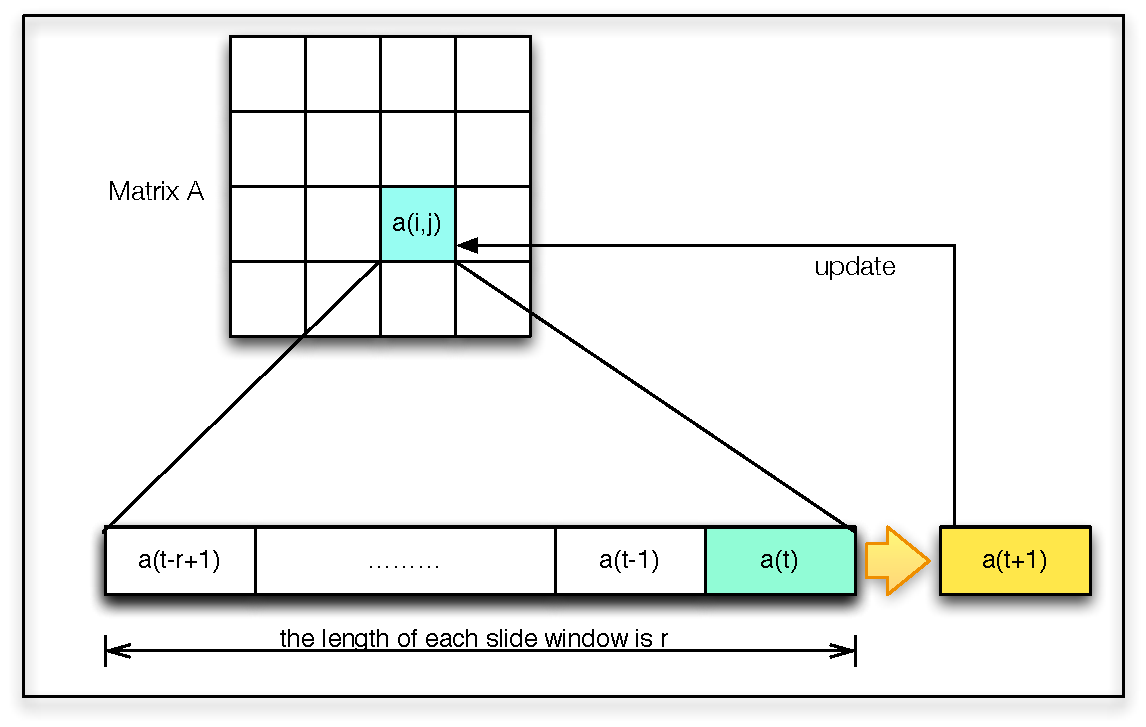
\includegraphics[width=0.7\textwidth]{paper-HCH/matrix}
  \caption{矩阵$\bm{A}$及其对应的滑动窗口}
  \label{fig:chap5_matrix}
\end{figure}

\begin{algorithm}[tbp] %算法的开始
\caption{Maintaining the matrix $\boldmath{A}$ and its slide-windows} %算法的标题
\label{alg:chap5_matrix} %给算法一个标签,这样方便在文中对算法的引用
\begin{algorithmic}[1] %这个1 表示每一行都显示数字
\REQUIRE  %算法的输入参数:Input
packet $M_k$, current time $t+1$
\ENSURE  %算法的输出:Output
matrix $\boldmath{A}$, slide-window $win$ \\
When packet $M_k$ comes\\
\textbf{local variables:} $i,j,c$
\STATE $i\leftarrow M_k.getSourceNodeID()$
\STATE $Sequence\leftarrow M_k.getPassedNodes()$
\STATE $c\leftarrow 1$
\FOR{$j\in Sequence$}
    \STATE $win[i,j,t]\leftarrow c$
    \STATE $c\leftarrow c+1$
\ENDFOR
\FOR{$i\leftarrow 1$ to $n$}
    \FOR{$j\leftarrow 1$ to $n$}
        \STATE $a_{i,j}\leftarrow \left(\sum_{k=t-r+1}^{k=t}win[i,j,k]\middle)\right/r$
    \ENDFOR
\ENDFOR
\RETURN $\boldmath{A}$, $win$ %算法的返回值
\end{algorithmic}
\end{algorithm}

\subsection{启发函数}
\label{chap5:启发函数}

\begin{equation}
\label{eq:H}
\mathcal{H}(i,k) = hop(k) + h(i, d)
\end{equation}

\begin{algorithm}[tbp] %算法的开始
\caption{Heuristic value calculation} %算法的标题
\label{alg:chap5_heuristic} %给算法一个标签,这样方便在文中对算法的引用
\begin{algorithmic}[1] %这个1 表示每一行都显示数字
\REQUIRE  %算法的输入参数:Input
Matrix $\boldmath{A}$ of node $i$
\ENSURE  %算法的输出:Output
$h(i,*)$\\
\textbf{local variables:} $i,h,c,d$ \\
\FOR{$M_k\in i.messages$}
    \STATE $h\leftarrow 0$
    \STATE $c\leftarrow 0$
    \STATE $M\leftarrow \Lambda$
    \STATE $i\leftarrow getHostID()$
    \STATE $d\leftarrow M_k.getDestinationID()$
    \REPEAT
        \STATE $M\leftarrow M\bigodot A$
        \STATE $h\leftarrow h+m_{i,d}$
        \STATE $c\leftarrow c+1$
    \UNTIL{$m_{i,d}=0$}
    \STATE $h(i,d)=h/c$
\ENDFOR
\RETURN $h(i,*)$ %算法的返回值
\end{algorithmic}
\end{algorithm}

\begin{figure}[bt]
  \centering
  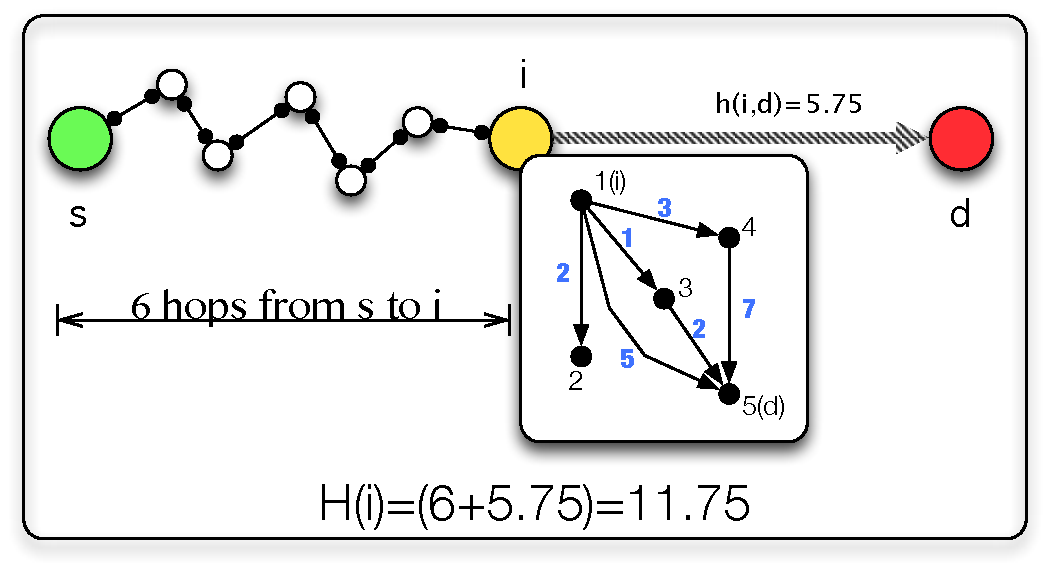
\includegraphics[width=0.6\textwidth]{paper-HCH/heuristic}
  \caption{跳数计算过程}
  \label{fig:heuristic}
\end{figure}

\section{路由协议}
\label{chap5:路由协议}

\begin{table}[bt]
  \caption{机会路由决策}
  \label{tab:chap5_routing}
  \centering
  \begin{tabular}{cc}
  \hline
   \textbf{策略:持有该消息的节点} & \textbf{对应情况}  \\
    \hline
    节点v和节点u & 向网络中增加一个新的消息副本\\
    节点v & 节点u不如节点v优\\
    u & 节点u比节点v优\\
    \hline
  \end{tabular}
\end{table}

\section{仿真实验}
\label{chap5:仿真实验}

\begin{table}
\centering
\caption{Helsinki City场景仿真设置}
\label{tab:simulation_helsinki}
\begin{tabular}{
p{0.45\linewidth}<{\centering}
p{0.5\linewidth}<{\centering}
}
\hline
\textbf{parameter name} & \textbf{range(default value)} \\
\hline
number of nodes & 120  \\
world size($m\times m$) & 4500$\times$3000  \\
tickets for S \& W & 13 \\
message TTL(min) & 200--500 (300) \\
simulation time(hours) & 12 \\
message size(KB) & 500--1024 \\
pedestrian buffer(MB) & 15--55 (15) \\
tram buffer(MB) & 500 \\
bluetooth range(m) & 10 \\
highspeed range(m) & 1000 \\ 
bluetooth bandwidth(KBps) & 250 \\
highspeed bandwidth(MBps) & 10 \\ 
pedestrian speed(m/s) & 0.5--1.5  \\
message interval(s) & 35--40 \\
\hline
\end{tabular}
\end{table}

\section{本章小结}
\label{chap5:本章小结}
%%==================================================
%% conclusion.tex for SJTU Master Thesis
%% based on CASthesis
%% modified by wei.jianwen@gmail.com
%% version: 0.3a
%% Encoding: UTF-8
%% last update: Dec 5th, 2010
%%==================================================

\chapter{总结及展望}
%\chapter*{总结及展望\markboth{总结及展望}{}}
%\addcontentsline{toc}{chapter}{全文总结}

目前,针对容迟网络的研究主要集中在路由协议领域,如何做出正确高效的路由选择是无线网络领域内的关键技术和主要研究课题。通过对近年来的主要研究成果进行分析,移动社会网络报文传输机制的研究是容迟网络研究在引入社会网络分析等技术后的最新发展趋势。最新的移动社会网络信息共享研究也是强调在容迟网络分布式体系结构下高容量、低成本的数据传输。本文基于移动模式最优节点群组选取算法,建立了周期相关的移动记录模型,并从移动记录中提取出节点(群组)移动模式。对于成组的节点,其被看做一个整体,并评估整体的预测投递率。本文对两个相关路由的关键属性进行研究分析,并将路由问题建模为组合最优化问题,且证明了该问题的$\mathcal{NP}$难解性。为求解该路由问题,基于局部搜索及禁忌搜索,分别提出了两种路由算法Local-MPAR及Tabu-MPAR。此外,证明了Tabu-MPAR过程可以使得持有消息的节点集合最终达到预测投递概率最优的集合。仿真实验表明:两种MPAR算法,在机会网络中的综合移动模型WDM上优于DF算法及SimBet算法。

本文基于消息传输收益的最优队列调度算法,针对节点间带宽和接触时间受限所导致的连接有限的吞吐量会造成消息的传输失败,从而浪费了节点间宝贵的接触机会的现象,通过定义概念“消息传输效用”,在PRoPHET的基础上加上数据项选择机制,得到改进后的路由算法Throughput。仿真实验表明:该数据项选择机制能够在消息投递率,消息投递时延,网络开销三方面较大程度的改进路由性能表现。

最后,本文利用启发函数,基于跳数信息进行消息投递跳数预测。利用滑动窗口机制,可以动态更新记录平均跳数的矩阵。基于此,定义了启发式函数用于预测当前节点到目的节点之间的潜在跳数。为了便于计算,定义了一种矩阵运算符,从而将跳数的估计过程转化为矩阵运算。仿真实验表明:本文提出的HCH算法在综合性能表现上优于Epidemic, S \& W以及PRoPHET三种算法。

智能交通系统所依赖的一种组网方式,即车联网,亦具有延迟容忍的特性,最新的研究趋势则是从延迟容忍网络及移动社会网络的角度,对车联网的路由问题进行研究。本文提出的基于移动模式的节点群组选取算法及对应的路由协议,正可用于社会属性相关的一类网络中。未来的研究将可集中于车联网的环境,针对车联网中既具有社会属性亦具有周期移动特性的一类节点进行分析,建立出能够如实反应其移动模式的数学模型,从而实现最优路由。此外,消息副本的分发速度是衡量路由性能的很重要的指标,本文对网络中消息副本分发速度只从仿真实验进行了验证,而未从理论上保证其可靠性。在以后的工作中,拟建立数学模型,对消息副本的分发过程进行分析,从理论上推导消息副本数量与分发时延之间的关系,从而保证消息的投递时延。

 %% 全文总结



%%%%%%%%%%%%%%%%%%%%%%%%%%%%%% 
%% 文后(无章节编号)
%%%%%%%%%%%%%%%%%%%%%%%%%%%%%% 
\backmatter

% 参考文献
% 使用 BibTeX
% 包含参考文献文件.bib
%\bibliography{reference/chap1,reference/chap2}
\bibliographystyle{ieeetr}
\bibliography{/Users/lei/Dropbox/papers.bib}

%% 个人简历(硕士学位论文没有个人简历要求)
% %%==================================================
%% resume.tex for SJTU Master Thesis
%% based on CASthesis
%% modified by wei.jianwen@gmail.com
%% version: 0.3a
%% Encoding: UTF-8
%% last update: Dec 5th, 2010
%%==================================================

\begin{resume}

\begin{resumesection}{基本情况}
xxx,男,上海人,1985 年~12 月出生,未婚,
上海交通大学物理系在读博士研究生。
\end{resumesection}

\begin{resumelist}{教育状况}
XXXX 年~9 月至~XXXX 年~7 月,上海交通大学, 本科,专业:XXXX

XXXX 年~9 月至~XXXX 年~7 月,上海交通大学, 硕士研究生,专业:XXXX

XXXX 年~9 月至~XXXX 年~7 月,上海交通大学,
博士研究生(提前攻读博士),专业:XXXX
\end{resumelist}

\begin{resumelist}{工作经历}
无。
\end{resumelist}

\begin{resumelist}{研究兴趣}
XXXXXXX。
\end{resumelist}

\begin{resumelist}{联系方式}
通讯地址:上海市闵行区东川路800号,上海交通大学物理系

邮编:200240

E-mail: abcde@sjtu.edu.cn
\end{resumelist}

\end{resume}


%\listoftables
%\listoffigures
%
%%\renewcommand{\listalgorithmcfname}{算法索引}
%\listofalgorithms

% 发表文章目录
%%==================================================
%% pub.tex for SJTU Master Thesis
%% based on CASthesis
%% modified by wei.jianwen@gmail.com
%% version: 0.3a
%% Encoding: UTF-8
%% last update: Dec 5th, 2010
%%==================================================



\begin{publications}{99}

%    \item\textsc{Chen H, Chan C~T}. {Acoustic cloaking in three dimensions using acoustic metamaterials}[J].
%      Applied Physics Letters, 2007, 91:183518.
%
%    \item\textsc{Chen H, Wu B~I, Zhang B}, et al. {Electromagnetic Wave Interactions with a Metamaterial Cloak}[J].
%      Physical Review Letters, 2007, 99(6):63903.

%\item\textsc{\textbf{L.~You}, J.~Li, C.~Wei, L.~Hu}, ``MPAR: A Movement Pattern-Aware Optimal Routing for Social Delay Tolerant Networks,'' in \textit{Ad Hoc Networks} (\textbf{SCI}, Impact Factor \textbf{1.943}), Vol.24, 2015, pp. 228-249.

\item MPAR: A Movement Pattern-Aware Optimal Routing for Social Delay Tolerant Networks, in \textit{Ad Hoc Networks} (\textbf{SCI}, Impact Factor \textbf{1.943}), Vol.24, 2015, pp. 228-249.

%
%\item\textsc{\textbf{L.~You}, L.~Lei, D.~Yuan}, ``On Power Optimization of Load-Coupled Heterogeneous LTE: Range Assignment via Offset,'' \textit{IEEE International Conference on Communication Systems (IEEE ICCS) 2014}, accepted

\item Range Assignment for Power Optimization in Load-Coupled Heterogeneous Networks, \textit{IEEE International Conference on Communication Systems (IEEE ICCS) 2014}, accepted

%
%\item\textsc{\textbf{L.~You}, L.~Lei, D.~Yuan}, ``A Performance Study of Energy Minimization for Interleaved and Localized FDMA,'' \textit{IEEE International Workshop on Computer-Aided Modeling Analysis and Design of Communication Links and Networks (IEEE CAMAD) 2014}, accepted

\item A Performance Study of Energy Minimization for Interleaved and Localized FDMA, \textit{IEEE International Workshop on Computer-Aided Modeling Analysis and Design of Communication Links and Networks (IEEE CAMAD) 2014}, accepted


%
%
%\item\textsc{\textbf{L.~You}, J.~Li, C.~Wei, C.~Dai}, ``A One-hop Information Based Geographic Routing Protocol for Delay Tolerant MANETs,'' in \textit{International Journal of Ad Hoc and Ubiquitous Computing} (\textbf{SCI}, Impact Factor \textbf{0.900}), in press.

\item A One-hop Information Based Geographic Routing Protocol for Delay Tolerant MANETs, in \textit{International Journal of Ad Hoc and Ubiquitous Computing} (\textbf{SCI}, Impact Factor \textbf{0.900}), in press.


%
%\item\textsc{\textbf{L.~You}, J.~Li, C.~Wei, C.~Dai, J.~Xu}, ``A General and Specific Utility Based Adaptive Routing for Delay Tolerant Networks,'' in \textit{International Journal of Distributed Sensor Networks} (\textbf{SCI}, Impact Factor \textbf{0.923}), Vol.2014, 15 pages, 2014.

\item A General and Specific Utility Based Adaptive Routing for Delay Tolerant Networks, in \textit{International Journal of Distributed Sensor Networks} (\textbf{SCI}, Impact Factor \textbf{0.923}), Vol.2014, 15 pages, 2014.

%
%\item\textsc{\textbf{L.~You}, J.~Li, C.~Wei, J.~Xu, C.~Dai}, ``A Data Item Selection Mechanism for Mobile Opportunistic Networks,'' in \textit{International Journal of Distributed Sensor Networks} (\textbf{SCI}, Impact Factor \textbf{0.923}), Vol.2014, 11 pages, 2014.

\item A Data Item Selection Mechanism for Mobile Opportunistic Networks, in \textit{International Journal of Distributed Sensor Networks} (\textbf{SCI}, Impact Factor \textbf{0.923}), Vol.2014, 11 pages, 2014.

%
%\item\textsc{\textbf{L.~You}, J.~Li, C.~Wei, C.~Dai, J.~Xu, L.~Hu}, ``A Hop Count Based Heuristic Routing Protocol for Mobile Delay Tolerant Networks'', in \textit{The Scientific World Journal} (\textbf{SCI}, Impact Factor \textbf{1.219}), Vol.2014, 12 pages, 2014.

\item A Hop Count Based Heuristic Routing Protocol for Mobile Delay Tolerant Networks, in \textit{The Scientific World Journal} (\textbf{SCI}, Impact Factor \textbf{1.219}), Vol.2014, 12 pages, 2014.

%
%\item\textsc{\textbf{L.~You}, Jianbo Li, Shan Jiang, Chenqu Dai}, ``A Hop Count Based Multi-path Forwarding Routing for Delay Tolerant Networks'', {\it Advances in Information Sciences and Service Sciences}, 5(7), pp.1199-1207, 2013.

\item A Hop Count Based Multi-path Forwarding Routing for Delay Tolerant Networks, in {\it Advances in Information Sciences and Service Sciences}, 5(7), pp.1199-1207, 2013.

\item 《面向社交信息分享的移动容迟网络消息传输研究》,山东省研究生优秀科技创新成果三等奖
    
\end{publications}




%% 参与项目列表
%%%==================================================
%% projects.tex for SJTU Master Thesis
%% based on CASthesis
%% modified by wei.jianwen@gmail.com
%% version: 0.3a
%% Encoding: UTF-8
%% last update: Dec 5th, 2010
%%==================================================

\begin{projects}{99}

    \item 973项目“XXX”
    \item 自然基金项目“XXX”
    \item 国防项目“XXX”
    
\end{projects}


%%%%%%%%%%%%%%%%%%%%%%%%%%%%%% 
%% 附录(章节编号重新计算,使用字母进行编号)
%%%%%%%%%%%%%%%%%%%%%%%%%%%%%% 
\appendix

% 附录中编号形式是"A-1"的样子
\renewcommand\theequation{\Alph{chapter}--\arabic{equation}}
\renewcommand\thefigure{\Alph{chapter}--\arabic{figure}}
\renewcommand\thetable{\Alph{chapter}--\arabic{table}}

%%%==================================================
%% app1.tex for SJTU Master Thesis
%% based on CASthesis
%% modified by wei.jianwen@gmail.com
%% version: 0.3a
%% Encoding: UTF-8
%% last update: Dec 5th, 2010
%%==================================================

\chapter{模板更新记录}
\label{chap:updatelog}

\textbf{2013年5月26日} v0.5.3发布,更正subsubsection格式错误,这个错误导致如"1.1 小结"这样的标题没有被正确加粗。

\textbf{2012年12月27日} v0.5.2发布,更正拼写错误:从``个人建立''更正为``个人简历''。在diss.tex加入ack.tex,更名后忘了引用。

\textbf{2012年12月21日} v0.5.1发布,在 \LaTeX 命令和中文字符之间留了空格,在Makefile中增加release功能。

\textbf{2012年12月5日} v0.5发布,修改说明文件的措辞,更正Makefile文件,使用metalog宏包替换xltxtra宏包,使用mathtools宏包替换amsmath宏包,移除了所有CJKtilde(\verb+~+)符号。

\textbf{2012年5月30日} v0.4发布,包含交大学士、硕士、博士学位论文模板。模板在\href{https://github.com/weijianwen/sjtu-thesis-template-latex}{github}上管理和更新。

\textbf{2010年12月5日} v0.3a发布,移植到 \XeTeX/\LaTeX 上。

\textbf{2009年12月25日} v0.2a发布,模板由CASthesis改名为sjtumaster。在diss.tex中可以方便地改变正文字号、切换但双面打印。增加了不编号的一章“全文总结”。
添加了可伸缩符号(等号、箭头)的例子,增加了长标题换行的例子。

\textbf{2009年11月20日} v0.1c发布,增加了Linux下使用ctex宏包的注意事项、.bib条目的规范要求,
修正了ctexbook与listings共同使用时的断页错误。

\textbf{2009年11月13日} v0.1b发布,完善了模板使用说明,增加了定理环境、并列子图、三线表格的例子。

\textbf{2009年11月12日} 上海交通大学硕士学位论文 \LaTeX 模板发布,版本0.1a。

 % 更新记录
%%% app2.tex for SJTU Master Thesis
%% based on CASthesis
%% modified by wei.jianwen@gmail.com
%% version: 0.3a
%% Encoding: UTF-8
%% last update: Dec 5th, 2010
%%==================================================

\chapter{Maxwell Equations}

选择二维情况,有如下的偏振矢量
\begin{subequations}
  \begin{eqnarray}
    {\bf E}&=&E_z(r,\theta)\hat{\bf z} \\
    {\bf H}&=&H_r(r,\theta))\hat{ \bf r}+H_\theta(r,\theta)\hat{\bm
      \theta}
  \end{eqnarray}
\end{subequations}
对上式求旋度
\begin{subequations}
  \begin{eqnarray}
    \nabla\times{\bf E}&=&\frac{1}{r}\frac{\partial E_z}{\partial\theta}{\hat{\bf r}}-\frac{\partial E_z}{\partial r}{\hat{\bm\theta}}\\
    \nabla\times{\bf H}&=&\left[\frac{1}{r}\frac{\partial}{\partial
        r}(rH_\theta)-\frac{1}{r}\frac{\partial
        H_r}{\partial\theta}\right]{\hat{\bf z}}
  \end{eqnarray}
\end{subequations}
因为在柱坐标系下,$\overline{\overline\mu}$是对角的,所以Maxwell方程组中电场$\bf
E$的旋度
\begin{subequations}
  \begin{eqnarray}
    &&\nabla\times{\bf E}=\mathbf{i}\omega{\bf B} \\
    &&\frac{1}{r}\frac{\partial E_z}{\partial\theta}{\hat{\bf
        r}}-\frac{\partial E_z}{\partial
      r}{\hat{\bm\theta}}=\mathbf{i}\omega\mu_rH_r{\hat{\bf r}}+\mathbf{i}\omega\mu_\theta
    H_\theta{\hat{\bm\theta}}
  \end{eqnarray}
\end{subequations}
所以$\bf H$的各个分量可以写为:
\begin{subequations}
  \begin{eqnarray}
    H_r=\frac{1}{\mathbf{i}\omega\mu_r}\frac{1}{r}\frac{\partial
      E_z}{\partial\theta } \\
    H_\theta=-\frac{1}{\mathbf{i}\omega\mu_\theta}\frac{\partial E_z}{\partial r}
  \end{eqnarray}
\end{subequations}
同样地,在柱坐标系下,$\overline{\overline\epsilon}$是对角的,所以Maxwell方程组中磁场$\bf
H$的旋度
\begin{subequations}
  \begin{eqnarray}
    &&\nabla\times{\bf H}=-\mathbf{i}\omega{\bf D}\\
    &&\left[\frac{1}{r}\frac{\partial}{\partial
        r}(rH_\theta)-\frac{1}{r}\frac{\partial
        H_r}{\partial\theta}\right]{\hat{\bf
        z}}=-\mathbf{i}\omega{\overline{\overline\epsilon}}{\bf
      E}=-\mathbf{i}\omega\epsilon_zE_z{\hat{\bf z}} \\
    &&\frac{1}{r}\frac{\partial}{\partial
      r}(rH_\theta)-\frac{1}{r}\frac{\partial
      H_r}{\partial\theta}=-\mathbf{i}\omega\epsilon_zE_z
  \end{eqnarray}
\end{subequations}
由此我们可以得到关于$E_z$的波函数方程:
\begin{eqnarray}
  \frac{1}{\mu_\theta\epsilon_z}\frac{1}{r}\frac{\partial}{\partial r}
  \left(r\frac{\partial E_z}{\partial r}\right)+
  \frac{1}{\mu_r\epsilon_z}\frac{1}{r^2}\frac{\partial^2E_z}{\partial\theta^2}
  +\omega^2 E_z=0
\end{eqnarray}
 % 麦克斯韦方程
% \include{body/app3}

%% 插图索引
%\listoffigures
%\addcontentsline{toc}{chapter}{\listfigurename} %将图索引加入全文目录
%% 表格索引
%\listoftables
%\addcontentsline{toc}{chapter}{\listtablename}  %将表格索引加入全文目录
%
%% 主要符号、缩略词对照表
%%%==================================================
%% symbol.tex for SJTU Master Thesis
%% based on CASthesis
%% modified by wei.jianwen@gmail.com
%% version: 0.3a
%% Encoding: UTF-8
%% last update: Dec 5th, 2010
%%==================================================

\chapter{主要符号对照表}
\label{chap:symb}
\begin{tabular}{ll}

 \hspace{2em}$\epsilon$       & \hspace{5em}介电常数 \\
 \hspace{2em}$\mu$ \qquad     & \hspace{5em}磁导率 \\
  \hspace{2em}$\epsilon$       & \hspace{5em}介电常数 \\
 \hspace{2em}$\mu$ \qquad     & \hspace{5em}磁导率 \\
 \hspace{2em}$\epsilon$       & \hspace{5em}介电常数 \\
 \hspace{2em}$\mu$ \qquad     & \hspace{5em}磁导率 \\
 \hspace{2em}$\epsilon$       & \hspace{5em}介电常数 \\
 \hspace{2em}$\mu$ \qquad     & \hspace{5em}磁导率 \\


\end{tabular}



% 致谢
%%==================================================
%% thanks.tex for SJTU Master Thesis
%% based on CASthesis
%% modified by wei.jianwen@gmail.com
%% version: 0.3a
%% Encoding: UTF-8
%% last update: Dec 5th, 2010
%%==================================================

\begin{thanks}

强烈感谢我的论文指导老师***教授,他们对我进行了无私的指导和帮助,不厌其烦的帮助进行论文的修改和改进。感谢我的女友***在我科研最困难的过程中给予我的关心和照顾,没有她的帮助,我很难想象自己如何支撑到科研工作最终完成那一刻。感谢在做论文的过程中,帮助我调整文档格式的各位同学们。另外,在校图书馆查找资料的时候,图书馆的老师也给我提供了很多方面的支持与 帮助。在此向帮助过我的老师致以真诚的谢意!



感谢这篇论文所涉及到的各位学者。本文引用了数位学者的研究文献,如果没有各位 学者的研究成果的帮助和启发,我将很难完成本篇论文的写作。
感谢我的同学和朋友,在我写论文的过程中给予我了很多重要素材,还在论文的撰写 和排版过程中提供热情的帮助。

  由于我的学术水平有限,所写论文难免有不足之处,恳请各位老师批评和指正!

\end{thanks}


% 论文原创性声明和使用授权
\makeDeclareOriginal

\end{document}
